
\section{For 2016 HEEP ID scale factor}
\label{AppHEEPsf_2016}
\subsection{N-1 (or N-2, N-3) efficiency for HEEP variables}
\label{AppHEEPsf_N_1_2016}
In order to find variables which cause the HEEP efficiency drop, one can look at N-1 or N-2 efficiencies and scale factors for various HEEP variables.
In 2016 the N-1, N-2 and N-3 efficiencies and scale factors are shown as functions of $E_T$, $\eta$ of the probe and of $N_{vtx}$ in figures \ref{fig:DEtaIn_2016}-\ref{fig:DetaIn_Dxy_DphiIn_2016}.

\begin{figure}[bh]
  \begin{center}
    \begin{tabular}{cc}
      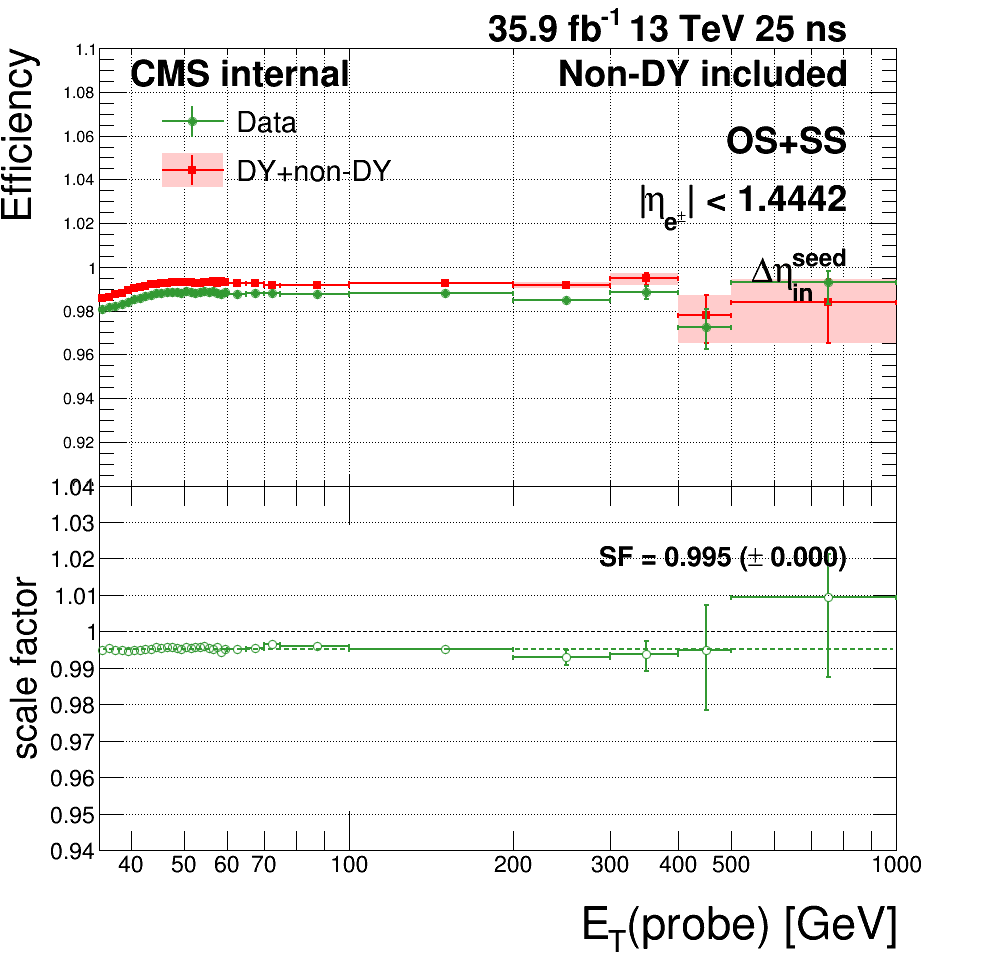
\includegraphics[width=0.45\textwidth]{figures/Zprime/2016/ScaleFactor/SameSign/N_1_eff/g_compare_cut_Et_Barrel_ea_ta_inc_AS_N_1_DEtaIn_PUW.png} &
      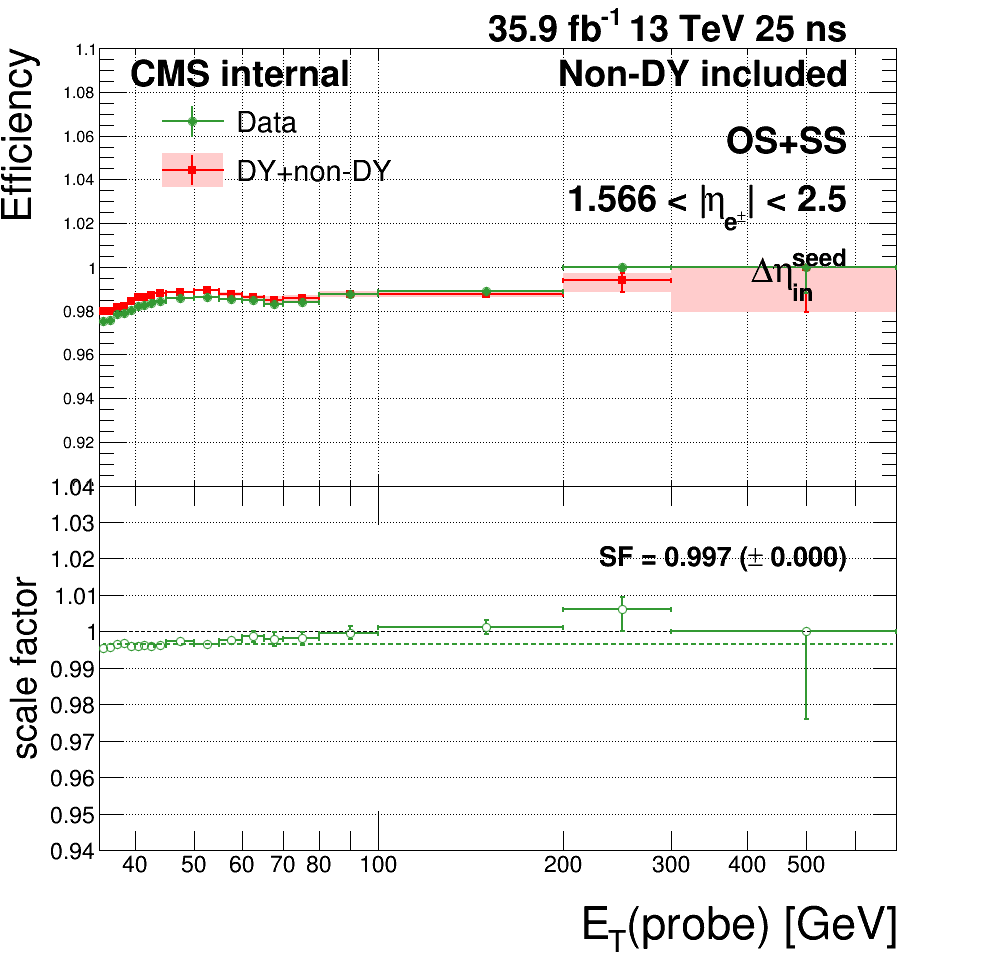
\includegraphics[width=0.45\textwidth]{figures/Zprime/2016/ScaleFactor/SameSign/N_1_eff/g_compare_cut_Et_Endcap_ea_ta_inc_AS_N_1_DEtaIn_PUW.png} \\
      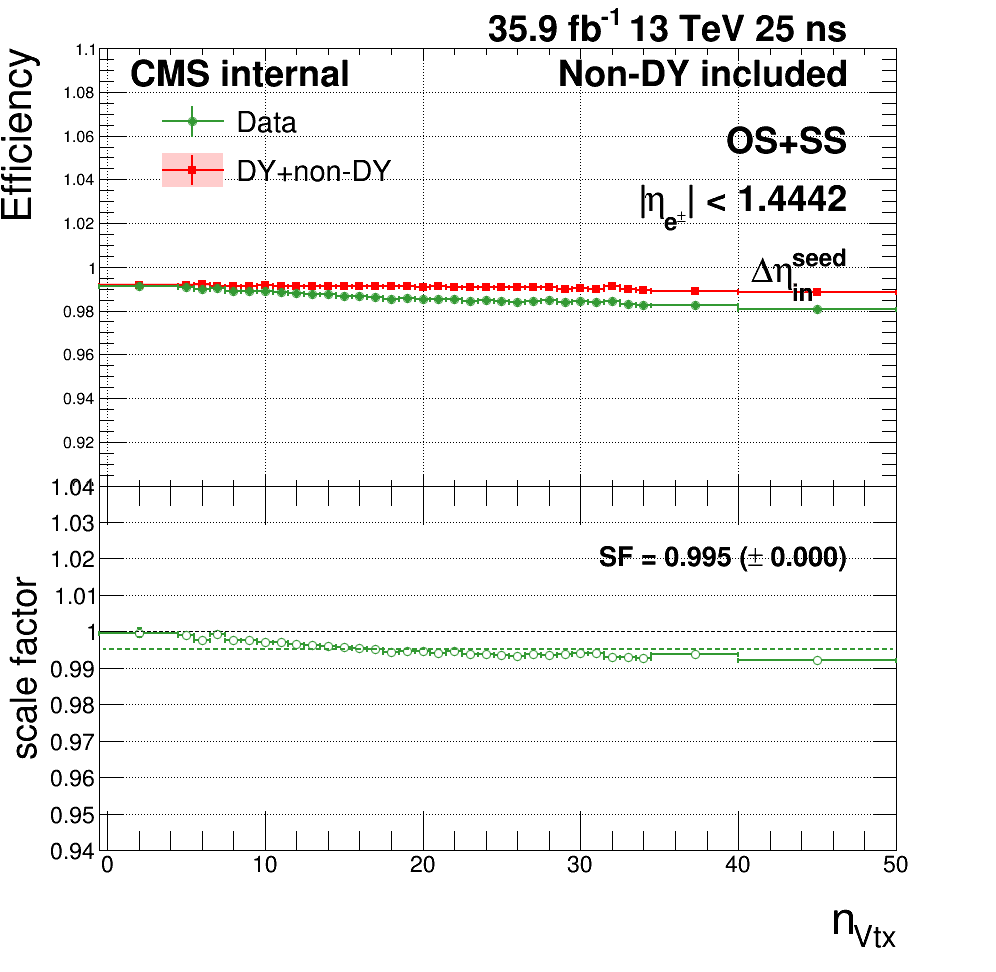
\includegraphics[width=0.45\textwidth]{figures/Zprime/2016/ScaleFactor/SameSign/N_1_eff/g_compare_cut_nVtx_Barrel_ea_ta_inc_AS_N_1_DEtaIn_PUW.png} &
      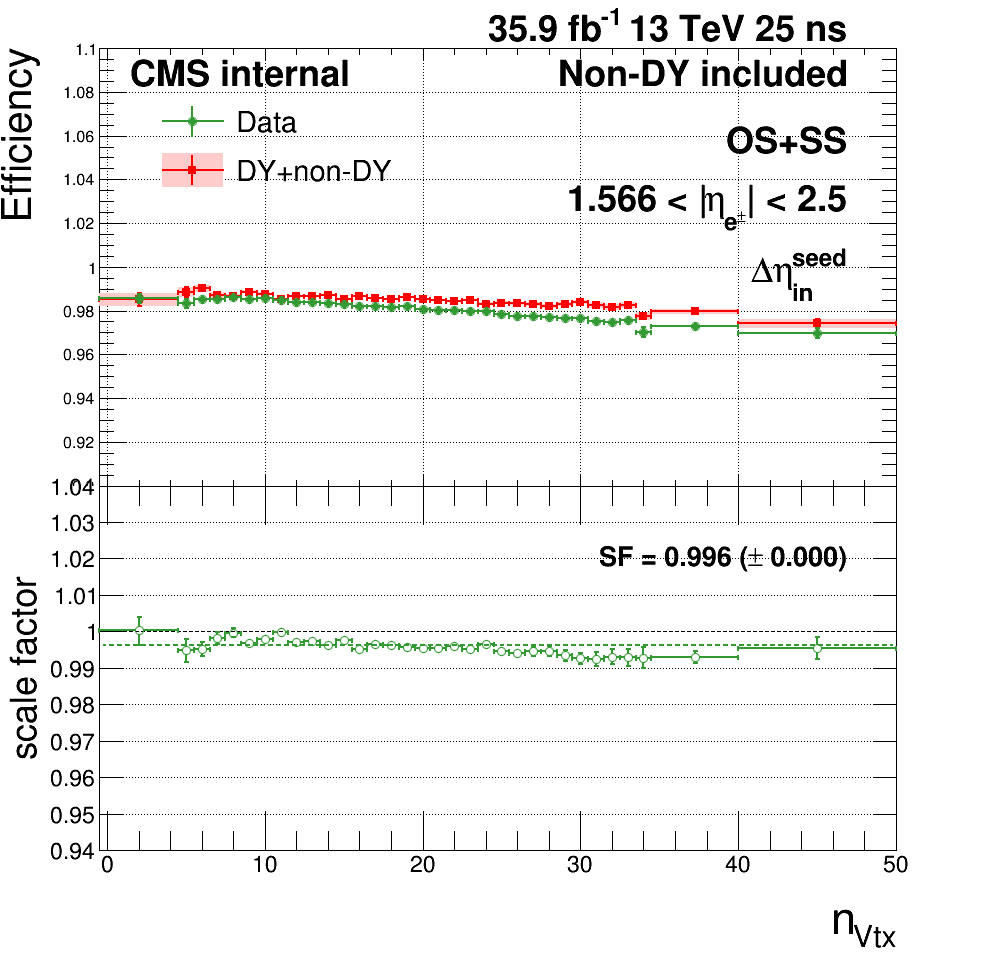
\includegraphics[width=0.45\textwidth]{figures/Zprime/2016/ScaleFactor/SameSign/N_1_eff/g_compare_cut_nVtx_Endcap_ea_ta_inc_AS_N_1_DEtaIn_PUW.png} \\
      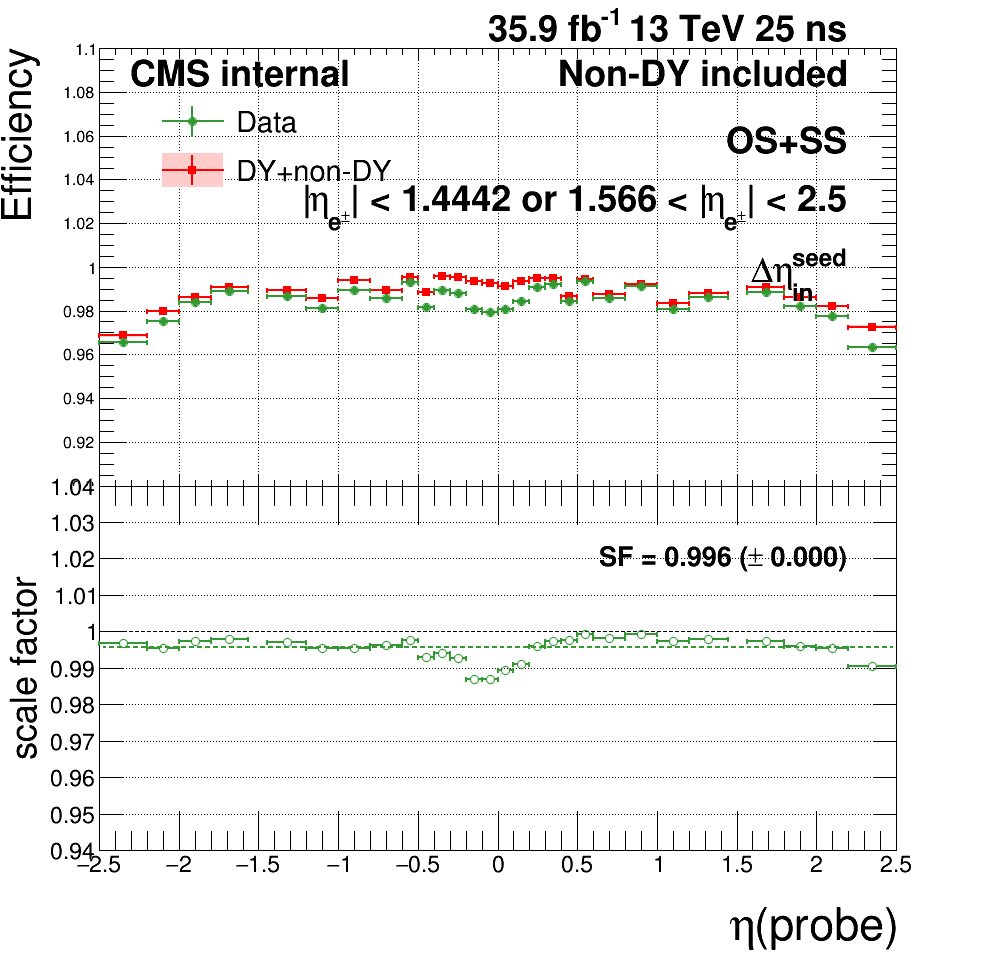
\includegraphics[width=0.45\textwidth]{figures/Zprime/2016/ScaleFactor/SameSign/N_1_eff/g_compare_cut_eta_Barrel+Endcap_ea_ta_inc_AS_N_1_DEtaIn_PUW.png}
    \end{tabular}
    \caption{$\Delta \eta_{in}^{seed}$ N-1 efficiencies and scale factors in MC and data in the barrel (left) and endcap (right) as functions of probe $E_T$ (top), $N_{vtx}$ (middle) and probe $\eta$ (bottom).}
    \label{fig:DEtaIn_2016}
  \end{center}
\end{figure}

\begin{figure}[bh]
  \begin{center}
    \begin{tabular}{cc}
      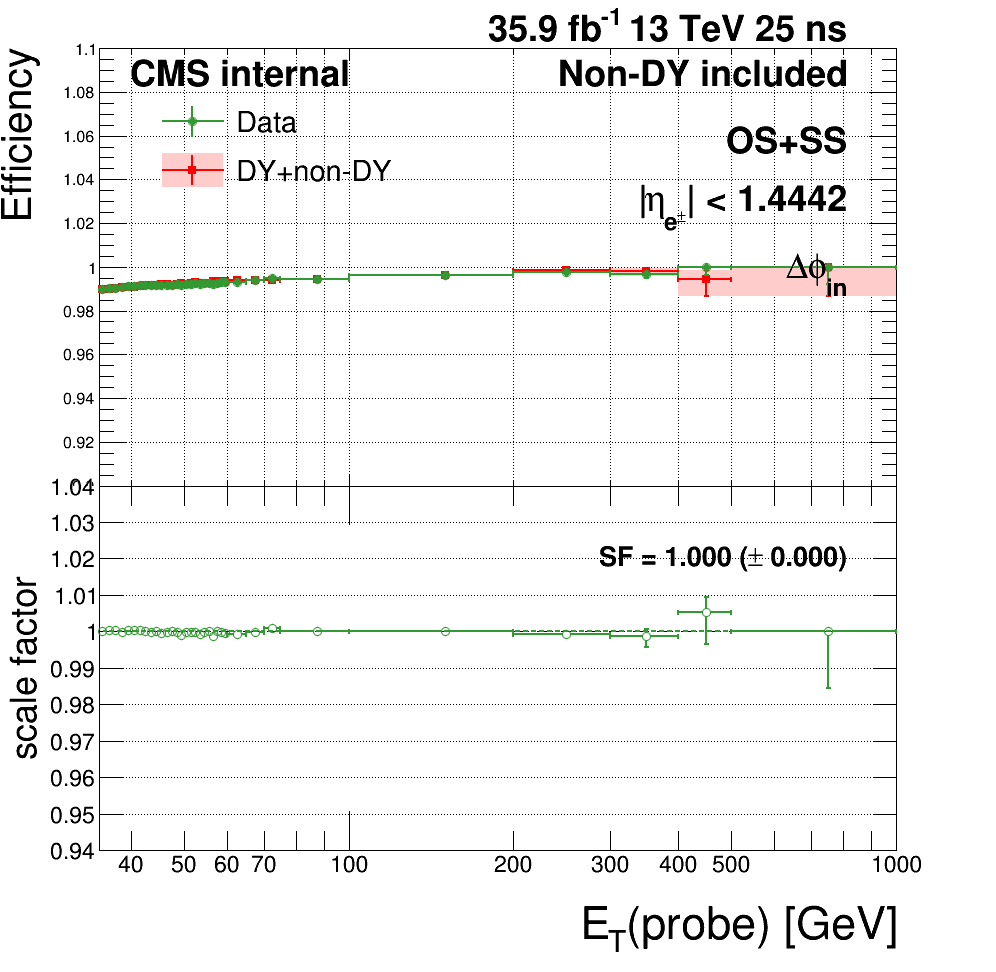
\includegraphics[width=0.45\textwidth]{figures/Zprime/2016/ScaleFactor/SameSign/N_1_eff/g_compare_cut_Et_Barrel_ea_ta_inc_AS_N_1_DPhiIn_PUW.png} &
      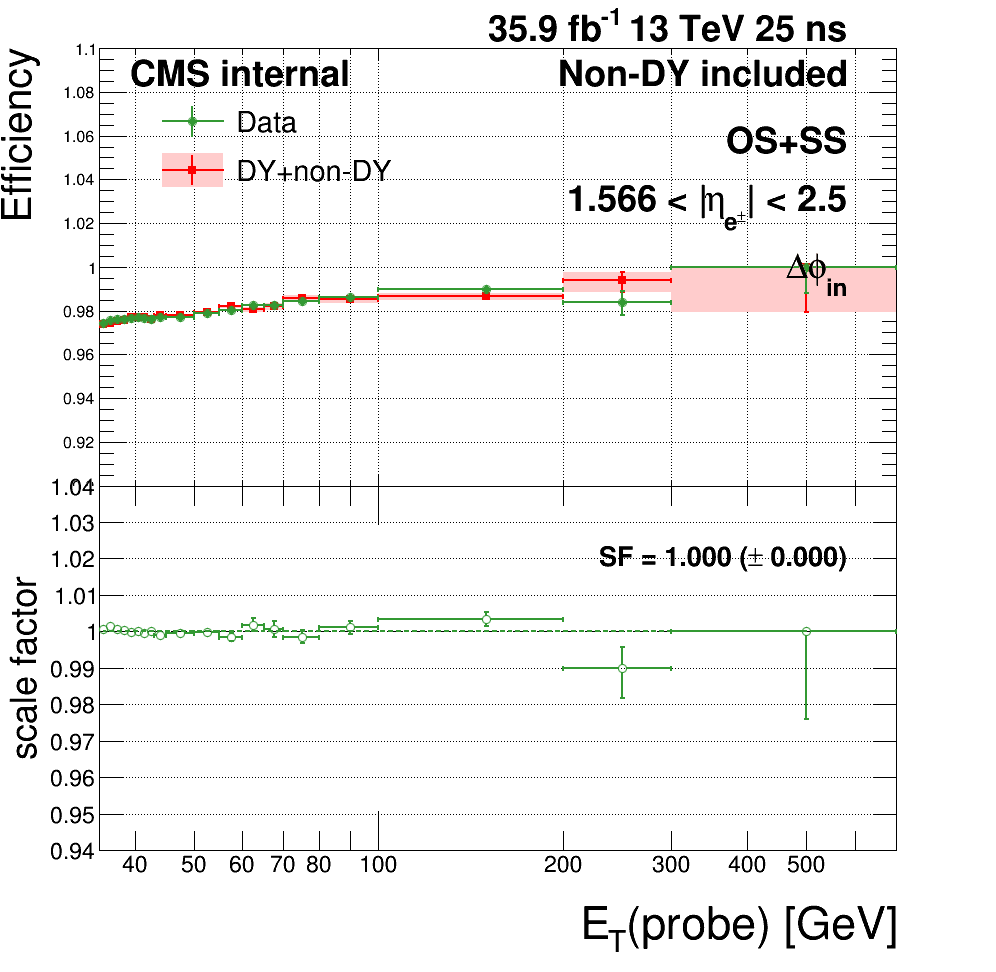
\includegraphics[width=0.45\textwidth]{figures/Zprime/2016/ScaleFactor/SameSign/N_1_eff/g_compare_cut_Et_Endcap_ea_ta_inc_AS_N_1_DPhiIn_PUW.png} \\
      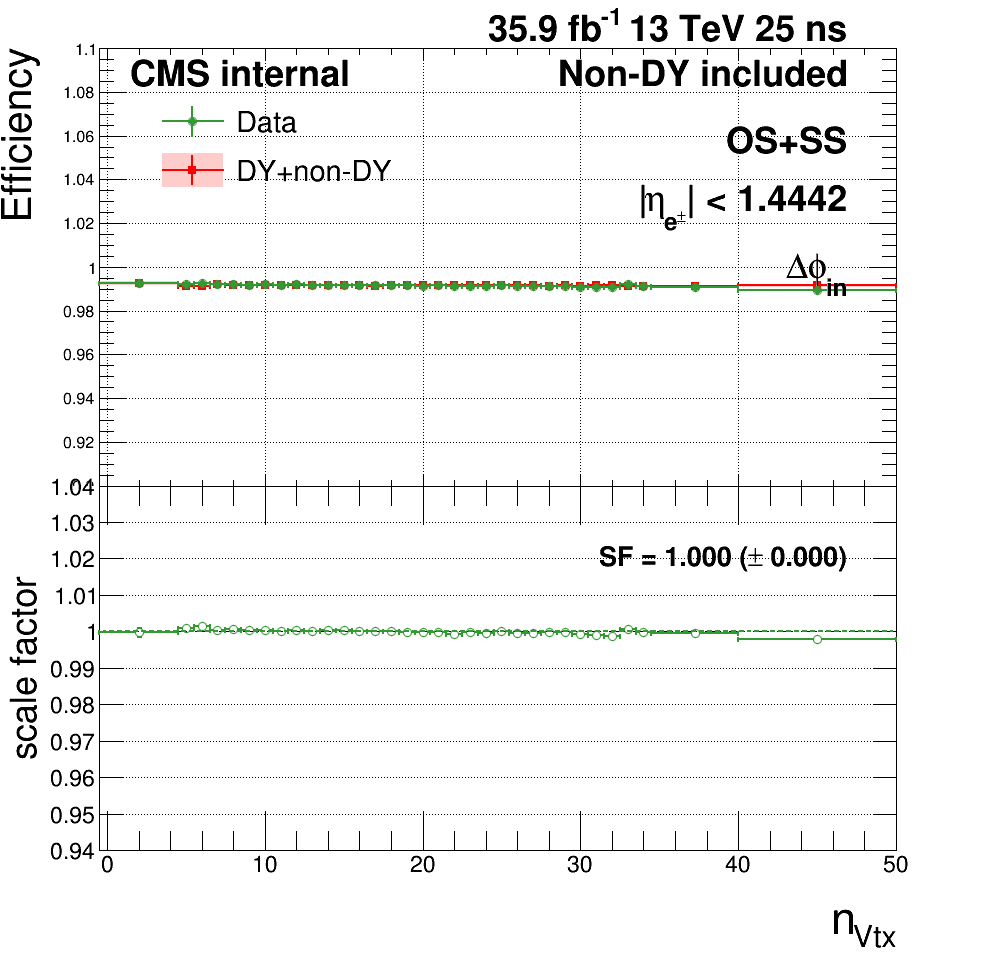
\includegraphics[width=0.45\textwidth]{figures/Zprime/2016/ScaleFactor/SameSign/N_1_eff/g_compare_cut_nVtx_Barrel_ea_ta_inc_AS_N_1_DPhiIn_PUW.png} &
      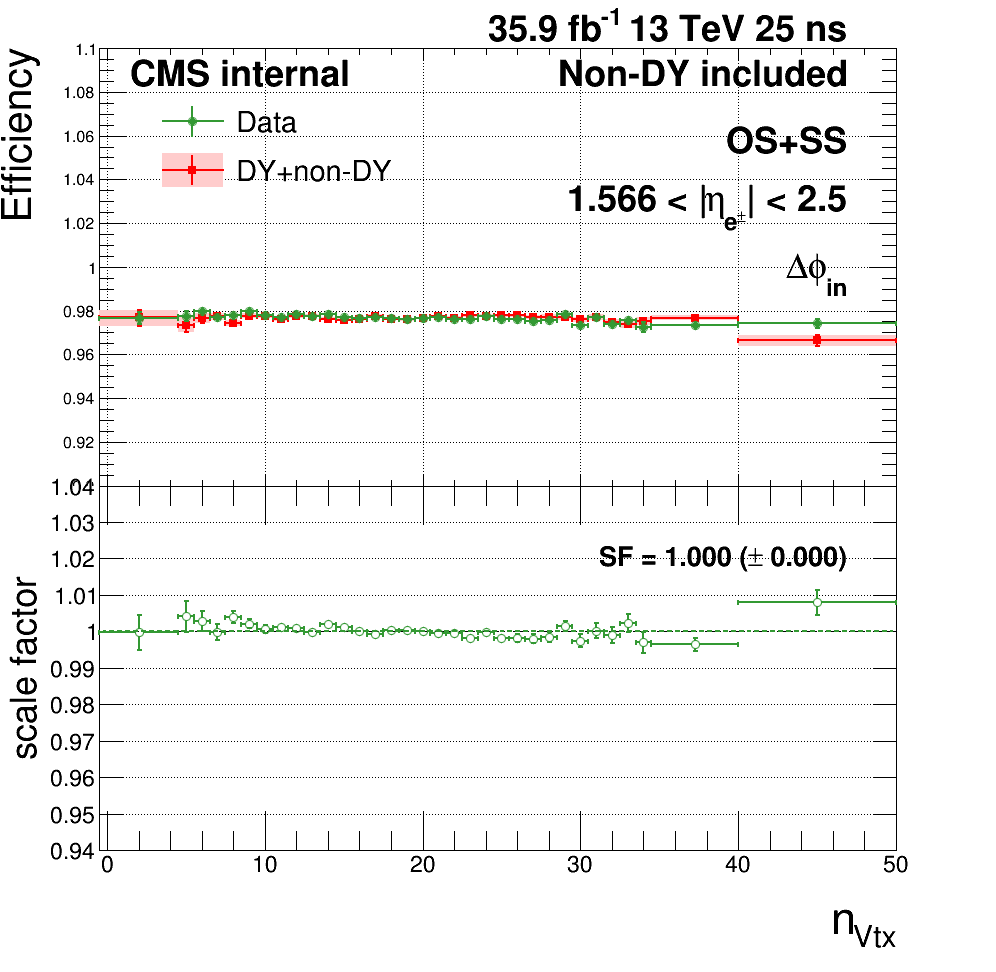
\includegraphics[width=0.45\textwidth]{figures/Zprime/2016/ScaleFactor/SameSign/N_1_eff/g_compare_cut_nVtx_Endcap_ea_ta_inc_AS_N_1_DPhiIn_PUW.png} \\
      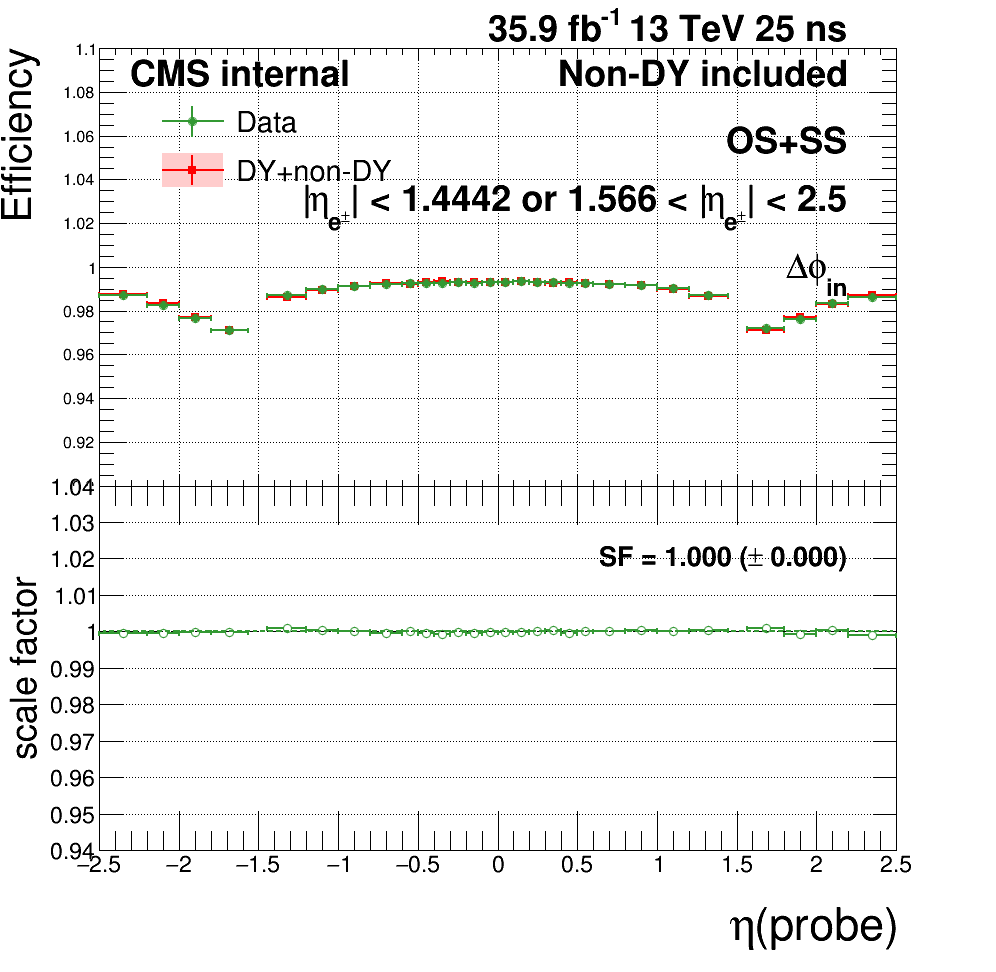
\includegraphics[width=0.45\textwidth]{figures/Zprime/2016/ScaleFactor/SameSign/N_1_eff/g_compare_cut_eta_Barrel+Endcap_ea_ta_inc_AS_N_1_DPhiIn_PUW.png}
    \end{tabular}
    \caption{$\Delta \phi_{in}$ N-1 efficiencies and scale factors in MC and data in the barrel (left) and endcap (right) as functions of probe $E_T$ (top), $N_{vtx}$ (middle) and probe $\eta$ (bottom).}
    \label{fig:DPhiIn_2016}
  \end{center}
\end{figure}

\begin{figure}[bh]
  \begin{center}
    \begin{tabular}{cc}
      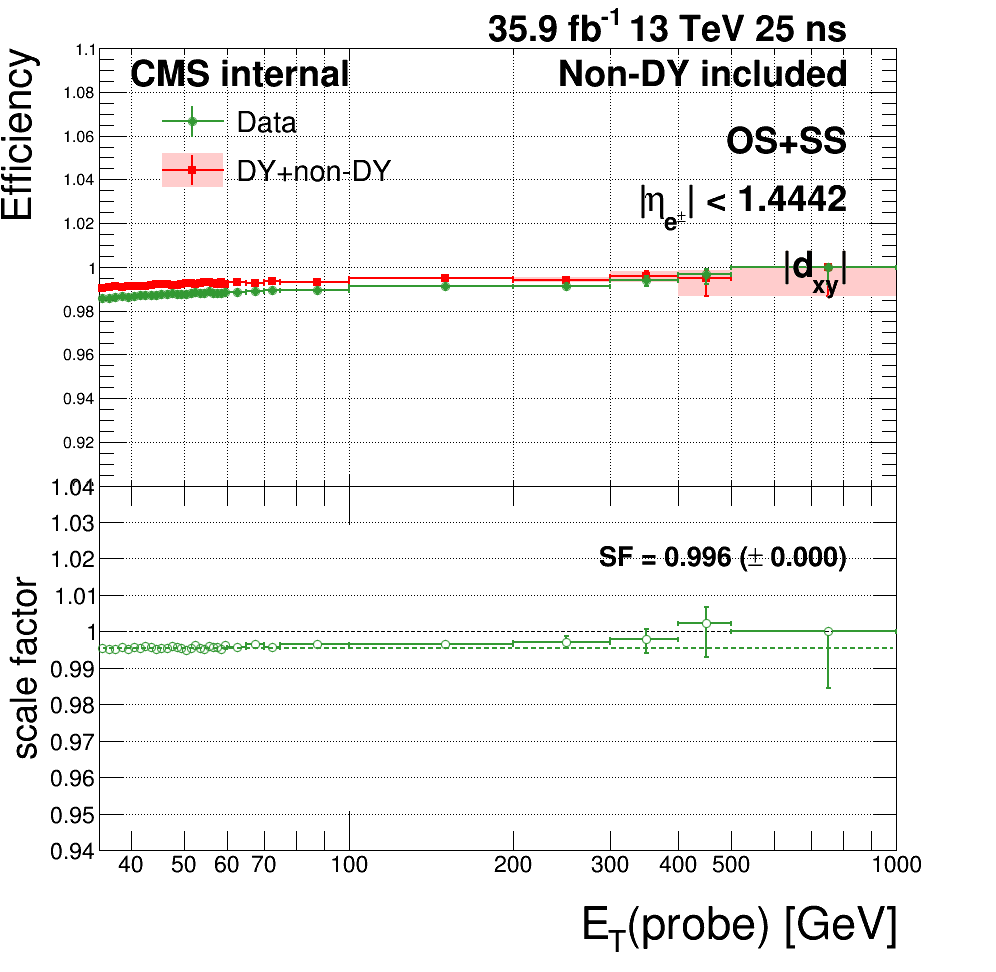
\includegraphics[width=0.45\textwidth]{figures/Zprime/2016/ScaleFactor/SameSign/N_1_eff/g_compare_cut_Et_Barrel_ea_ta_inc_AS_N_1_Dxy_PUW.png} &
      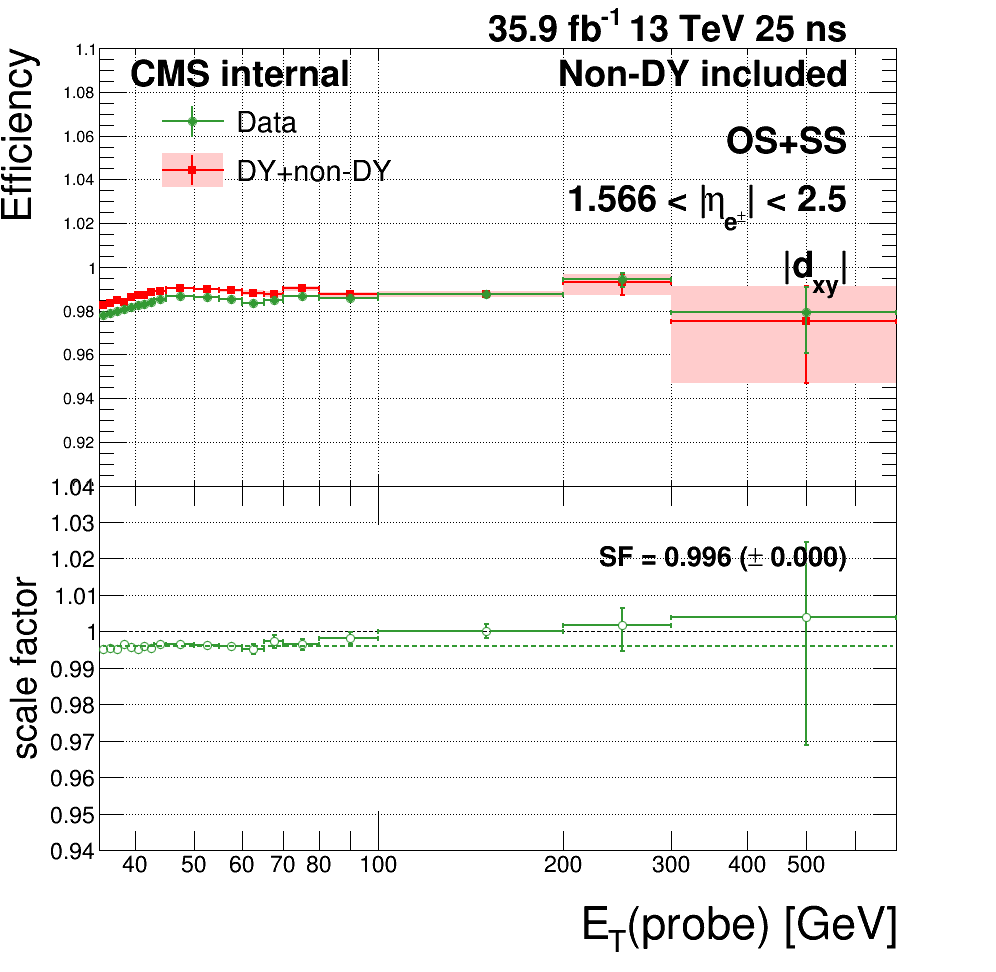
\includegraphics[width=0.45\textwidth]{figures/Zprime/2016/ScaleFactor/SameSign/N_1_eff/g_compare_cut_Et_Endcap_ea_ta_inc_AS_N_1_Dxy_PUW.png} \\
      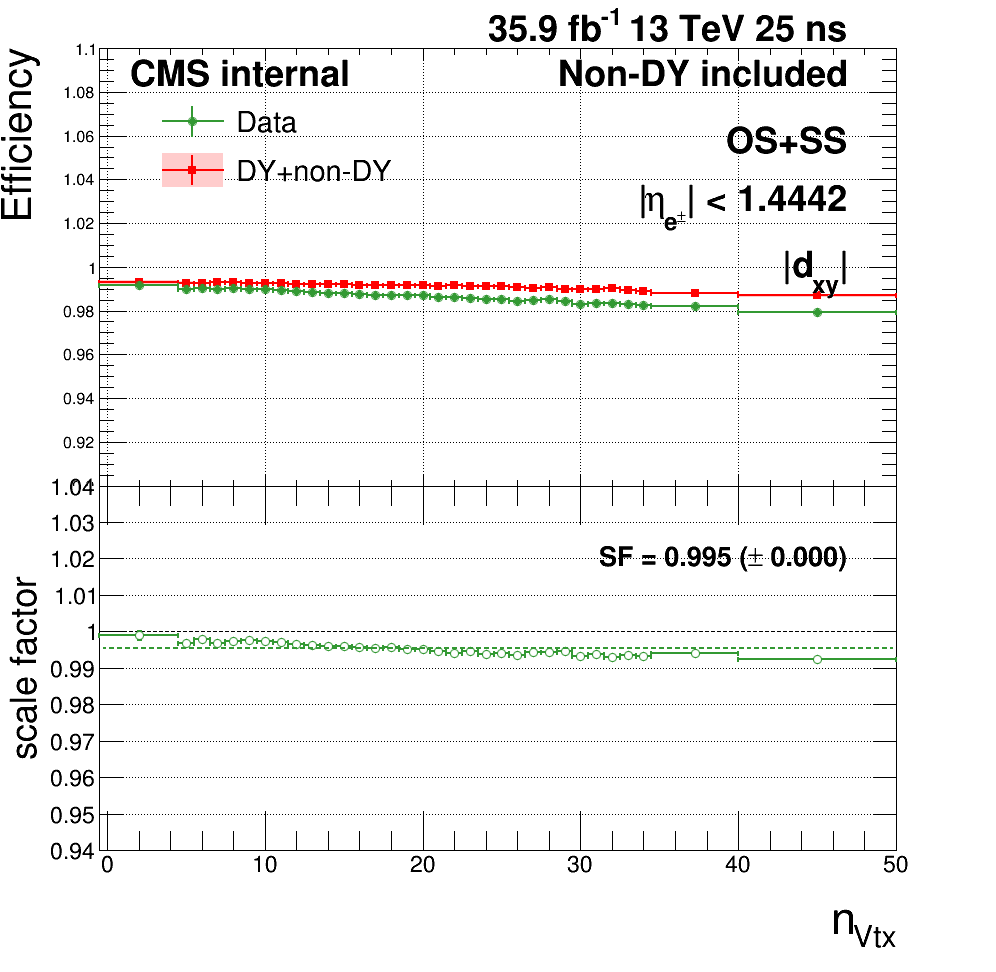
\includegraphics[width=0.45\textwidth]{figures/Zprime/2016/ScaleFactor/SameSign/N_1_eff/g_compare_cut_nVtx_Barrel_ea_ta_inc_AS_N_1_Dxy_PUW.png} &
      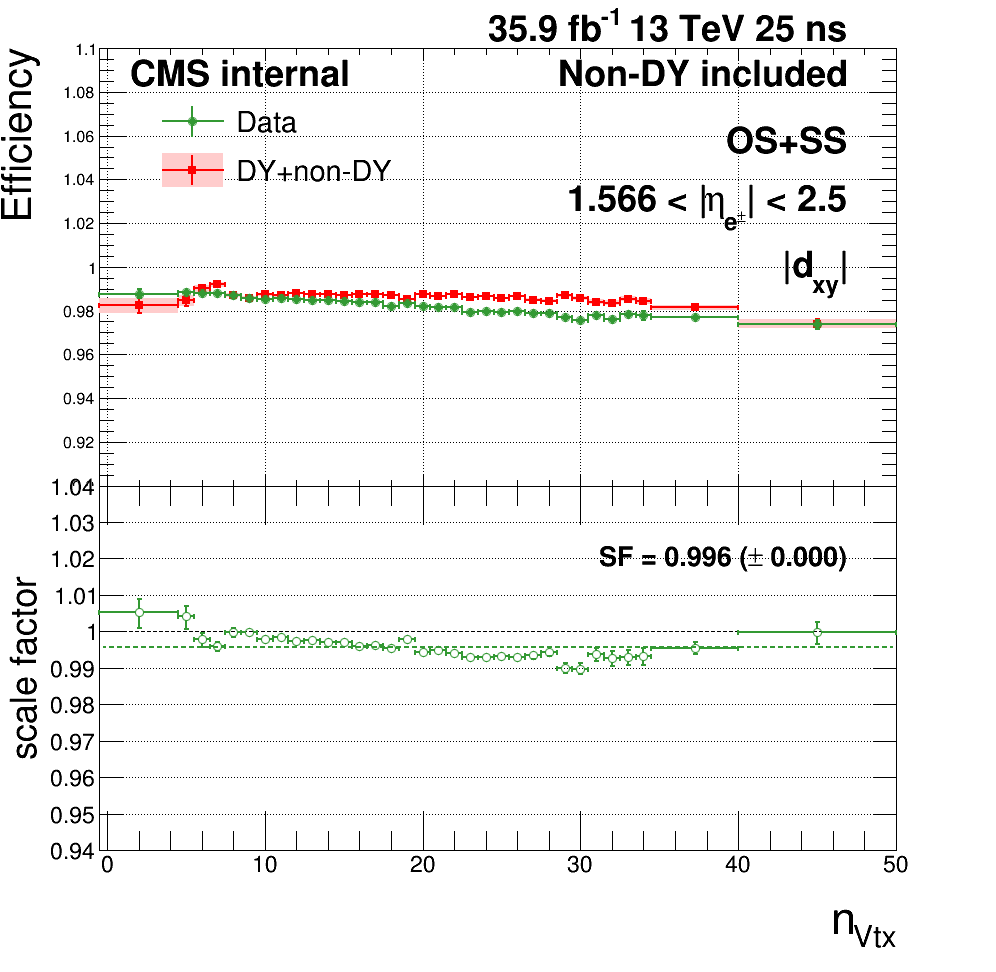
\includegraphics[width=0.45\textwidth]{figures/Zprime/2016/ScaleFactor/SameSign/N_1_eff/g_compare_cut_nVtx_Endcap_ea_ta_inc_AS_N_1_Dxy_PUW.png} \\
      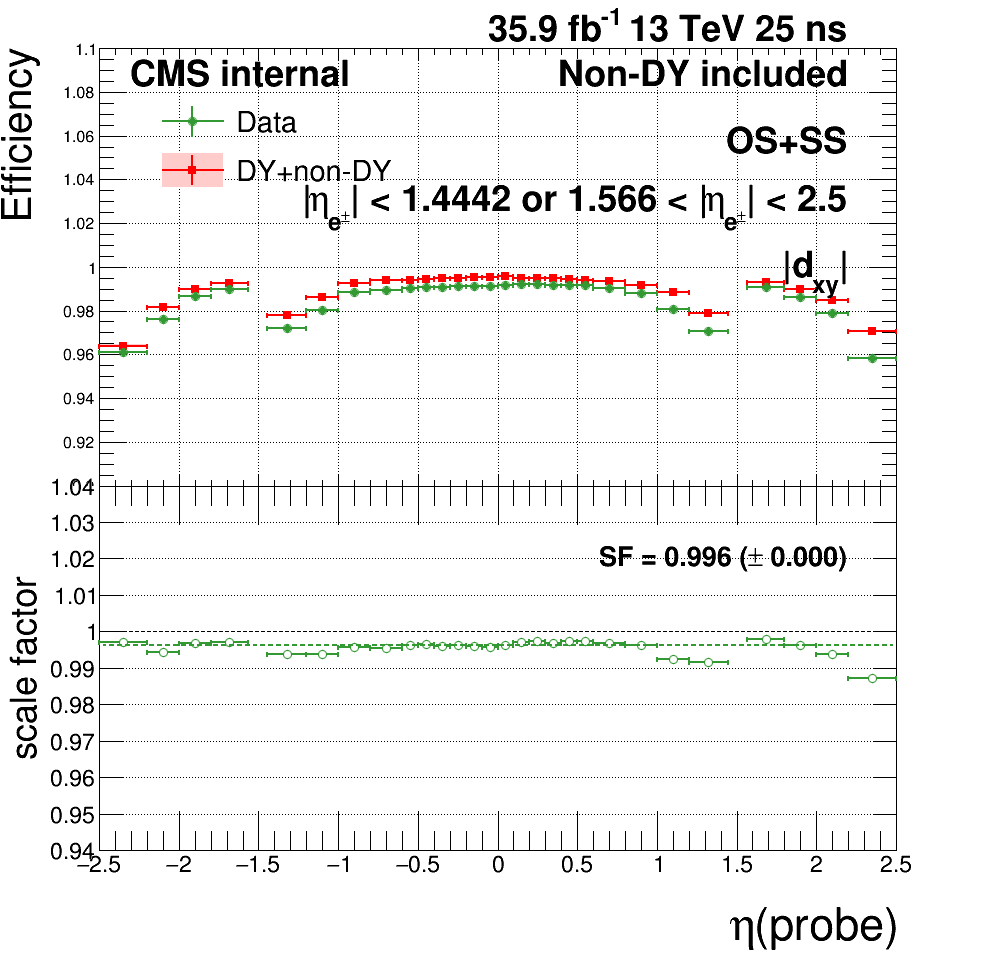
\includegraphics[width=0.45\textwidth]{figures/Zprime/2016/ScaleFactor/SameSign/N_1_eff/g_compare_cut_eta_Barrel+Endcap_ea_ta_inc_AS_N_1_Dxy_PUW.png}
    \end{tabular}
    \caption{$|d_{xy}|$ N-1 efficiencies and scale factors in MC and data in the barrel (left) and endcap (right) as functions of probe $E_T$ (top), $N_{vtx}$ (middle) and probe $\eta$ (bottom).}
    \label{fig:Dxy_2016}
  \end{center}
\end{figure}

\begin{figure}[bh]
  \begin{center}
    \begin{tabular}{cc}
      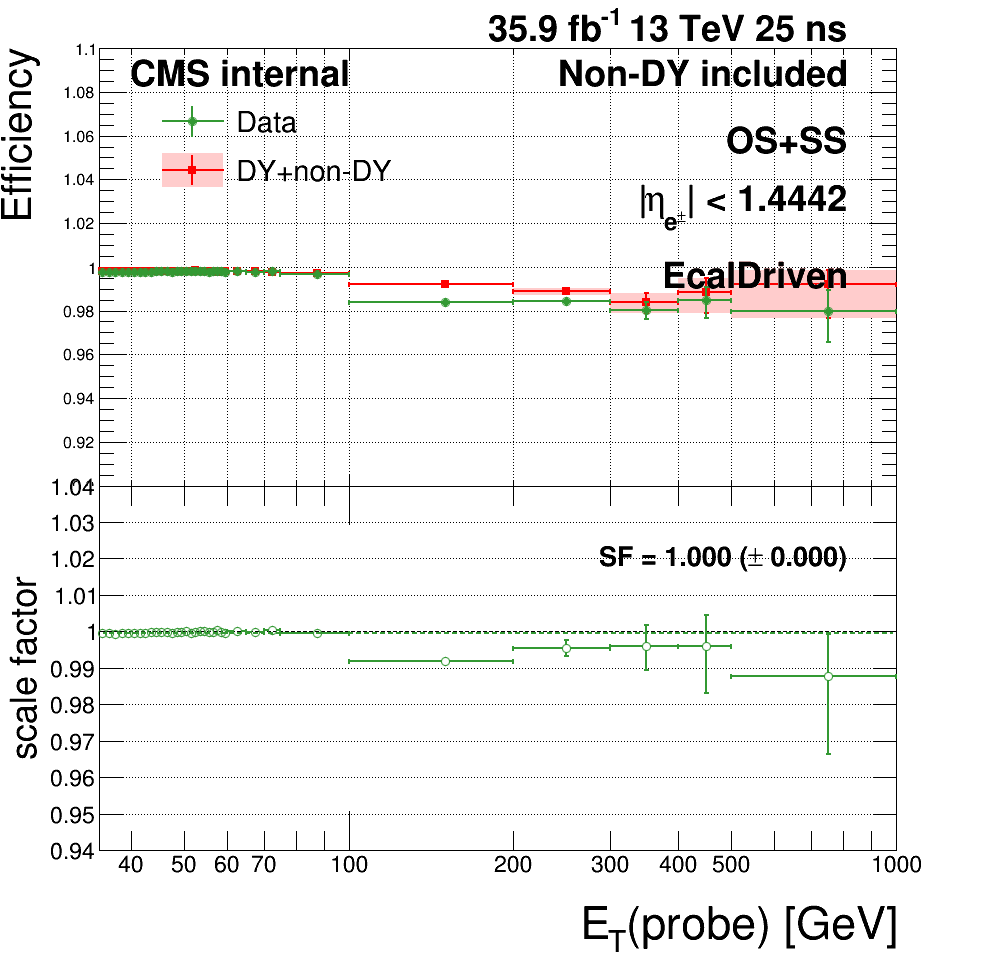
\includegraphics[width=0.45\textwidth]{figures/Zprime/2016/ScaleFactor/SameSign/N_1_eff/g_compare_cut_Et_Barrel_ea_ta_inc_AS_N_1_EcalDriven_PUW.png} &
      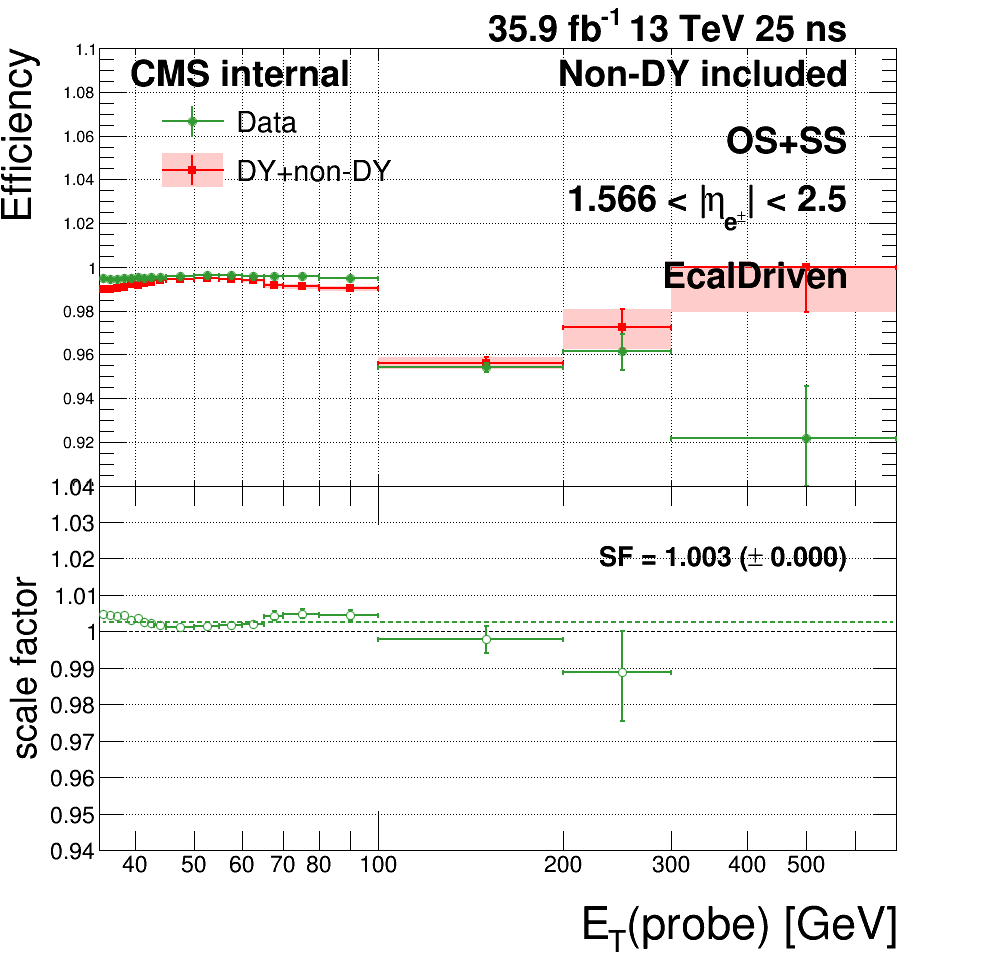
\includegraphics[width=0.45\textwidth]{figures/Zprime/2016/ScaleFactor/SameSign/N_1_eff/g_compare_cut_Et_Endcap_ea_ta_inc_AS_N_1_EcalDriven_PUW.png} \\
      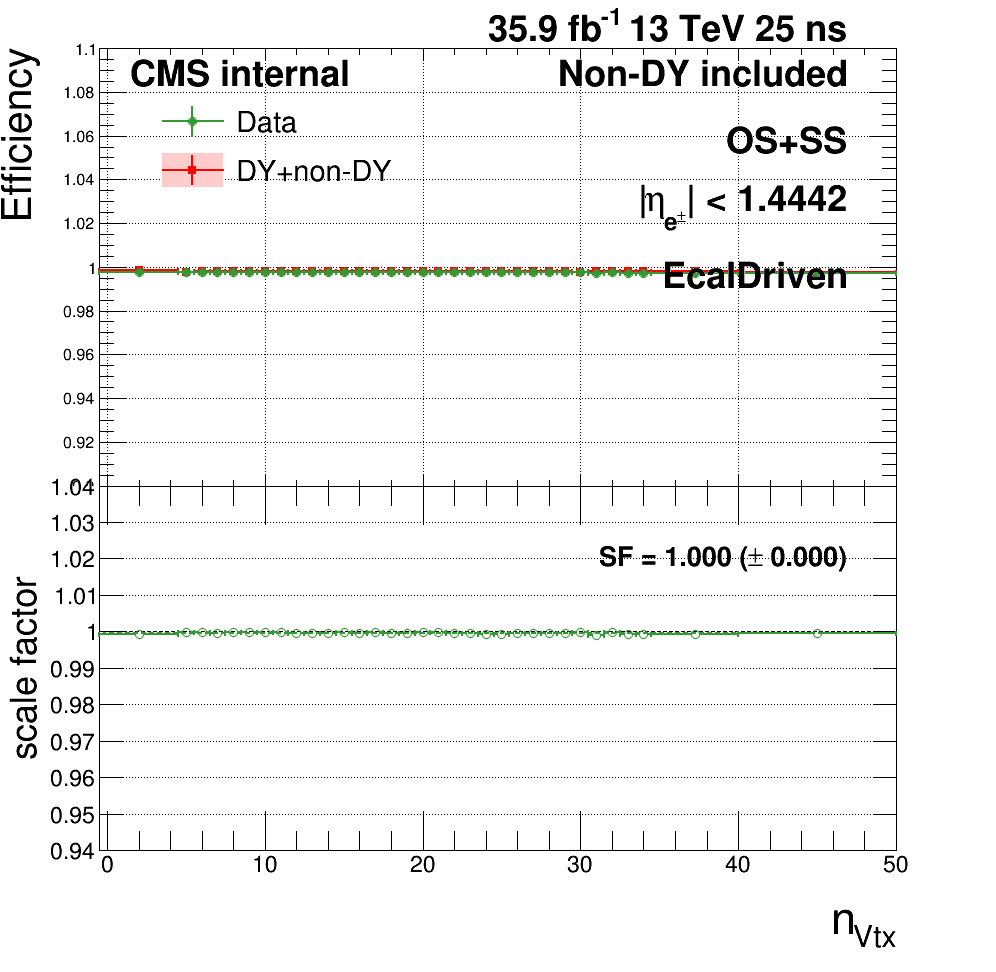
\includegraphics[width=0.45\textwidth]{figures/Zprime/2016/ScaleFactor/SameSign/N_1_eff/g_compare_cut_nVtx_Barrel_ea_ta_inc_AS_N_1_EcalDriven_PUW.png} &
      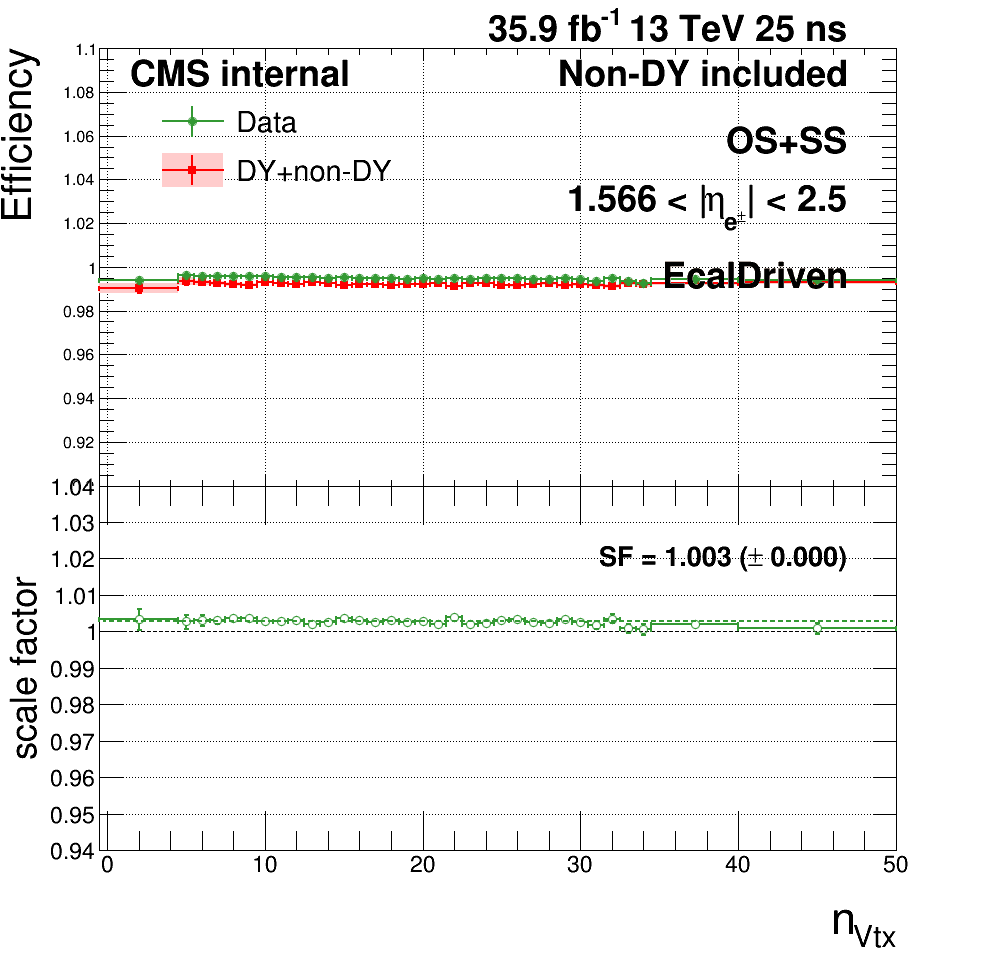
\includegraphics[width=0.45\textwidth]{figures/Zprime/2016/ScaleFactor/SameSign/N_1_eff/g_compare_cut_nVtx_Endcap_ea_ta_inc_AS_N_1_EcalDriven_PUW.png} \\
      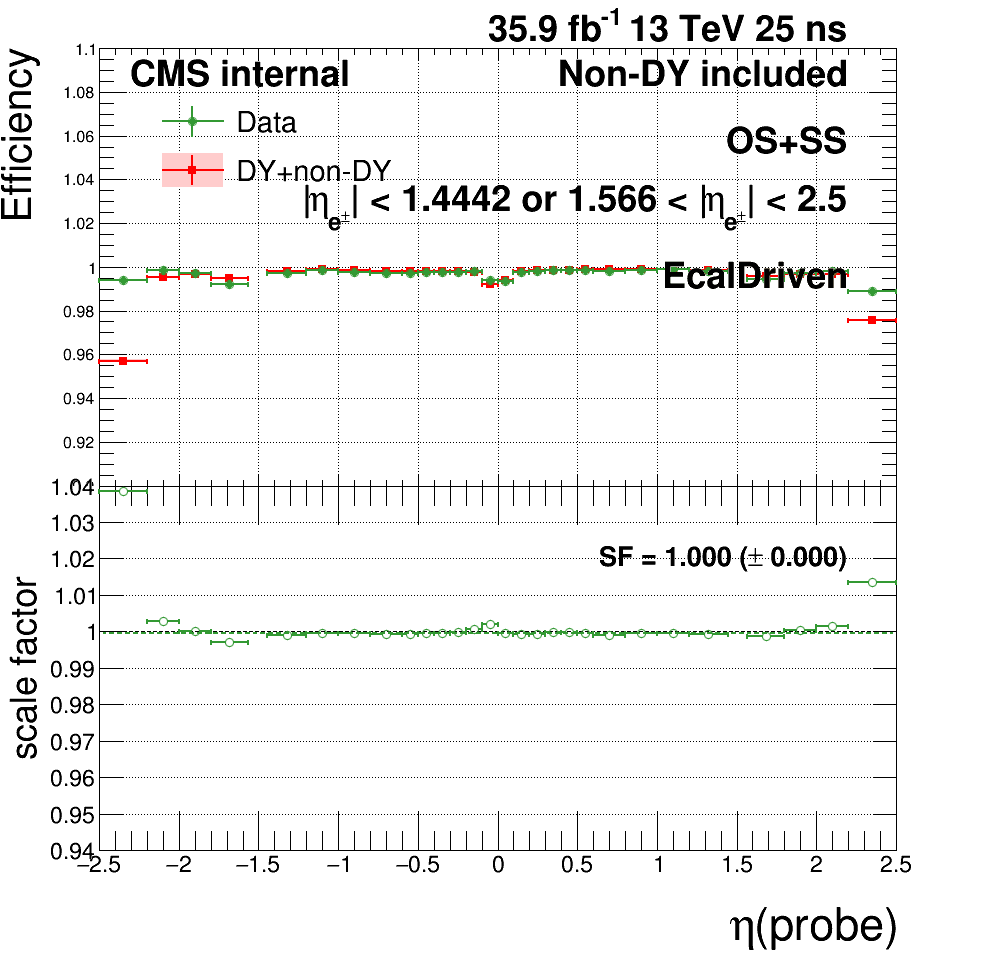
\includegraphics[width=0.45\textwidth]{figures/Zprime/2016/ScaleFactor/SameSign/N_1_eff/g_compare_cut_eta_Barrel+Endcap_ea_ta_inc_AS_N_1_EcalDriven_PUW.png}
    \end{tabular}
    \caption{$EcalDriven$ N-1 efficiencies and scale factors in MC and data in the barrel (left) and endcap (right) as functions of probe $E_T$ (top), $N_{vtx}$ (middle) and probe $\eta$ (bottom).}
    \label{fig:EcalDriven_2016}
  \end{center}
\end{figure}

\begin{figure}[bh]
  \begin{center}
    \begin{tabular}{cc}
      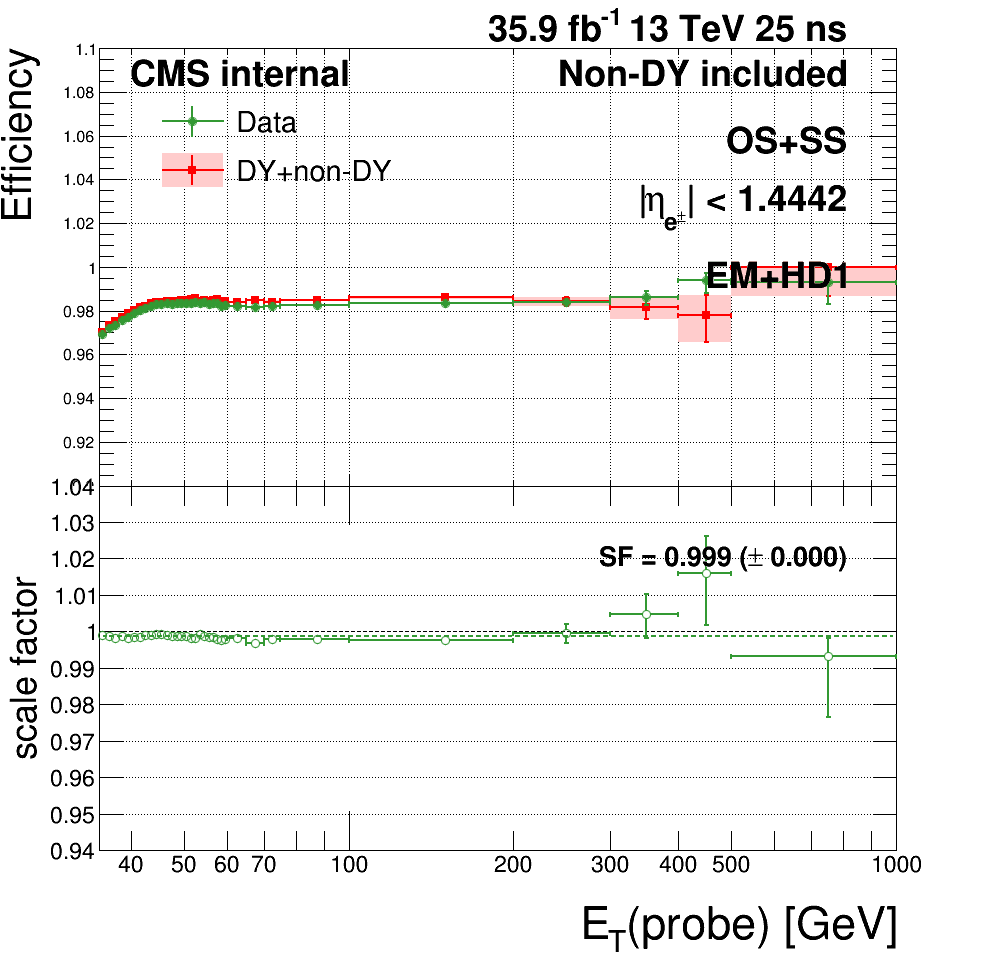
\includegraphics[width=0.45\textwidth]{figures/Zprime/2016/ScaleFactor/SameSign/N_1_eff/g_compare_cut_Et_Barrel_ea_ta_inc_AS_N_1_EMHD1Iso_PUW.png} &
      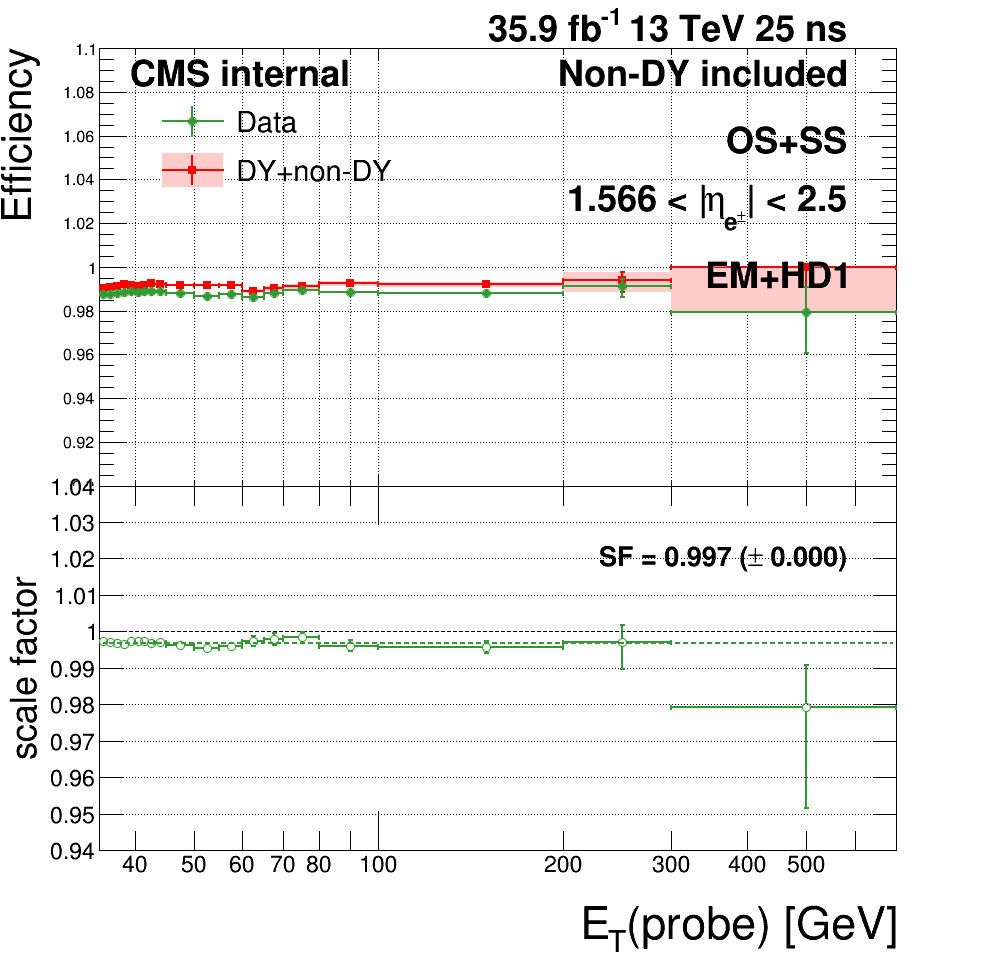
\includegraphics[width=0.45\textwidth]{figures/Zprime/2016/ScaleFactor/SameSign/N_1_eff/g_compare_cut_Et_Endcap_ea_ta_inc_AS_N_1_EMHD1Iso_PUW.png} \\
      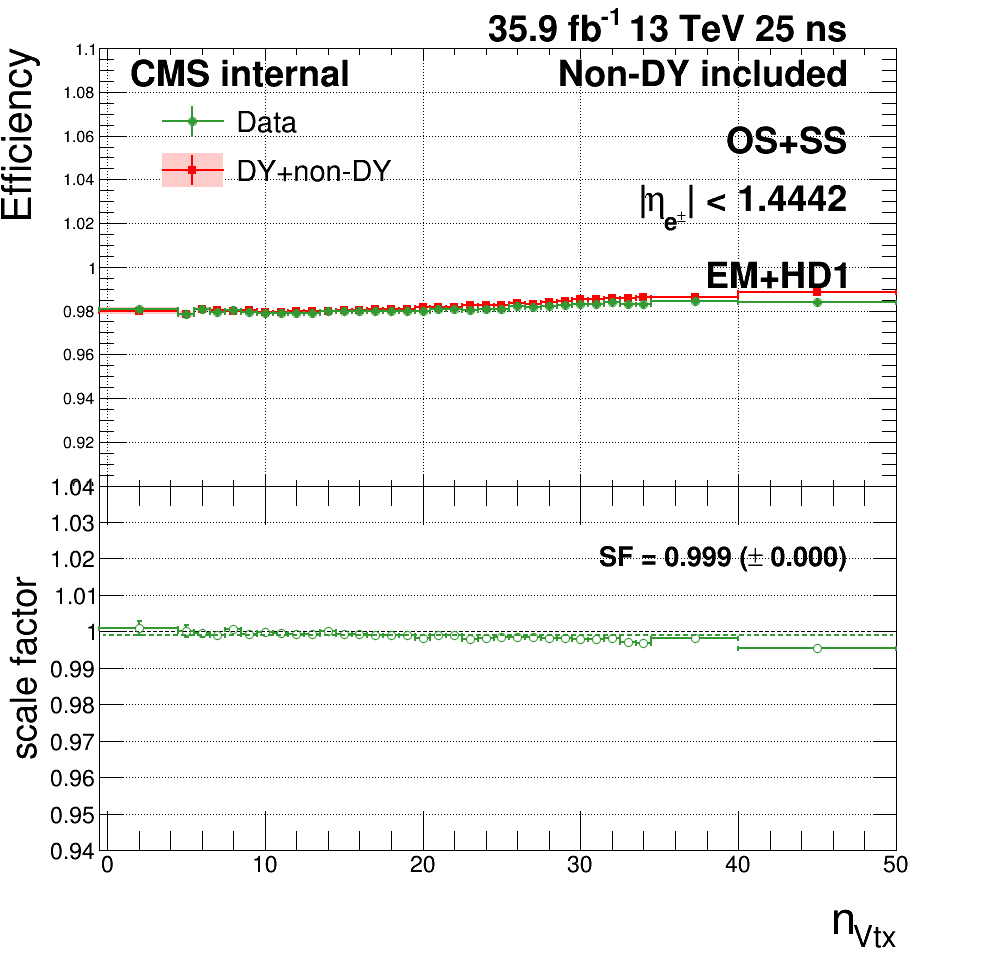
\includegraphics[width=0.45\textwidth]{figures/Zprime/2016/ScaleFactor/SameSign/N_1_eff/g_compare_cut_nVtx_Barrel_ea_ta_inc_AS_N_1_EMHD1Iso_PUW.png} &
      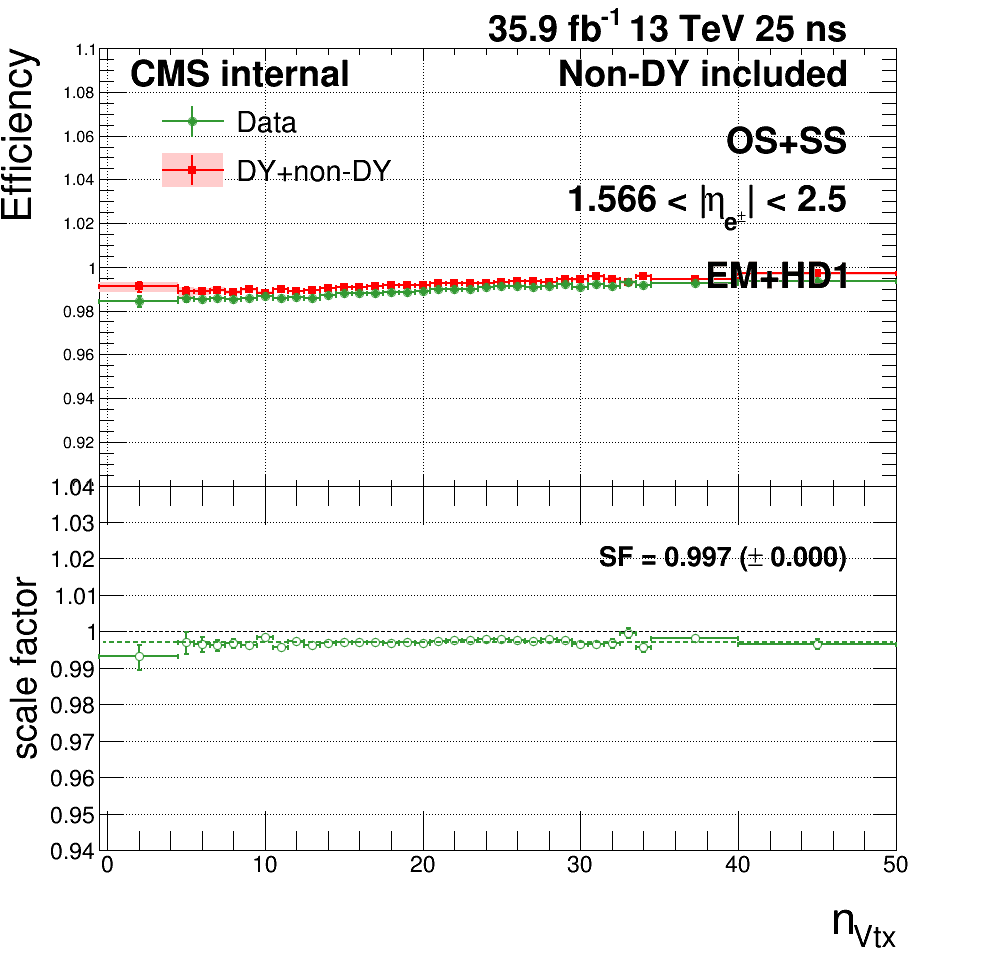
\includegraphics[width=0.45\textwidth]{figures/Zprime/2016/ScaleFactor/SameSign/N_1_eff/g_compare_cut_nVtx_Endcap_ea_ta_inc_AS_N_1_EMHD1Iso_PUW.png} \\
      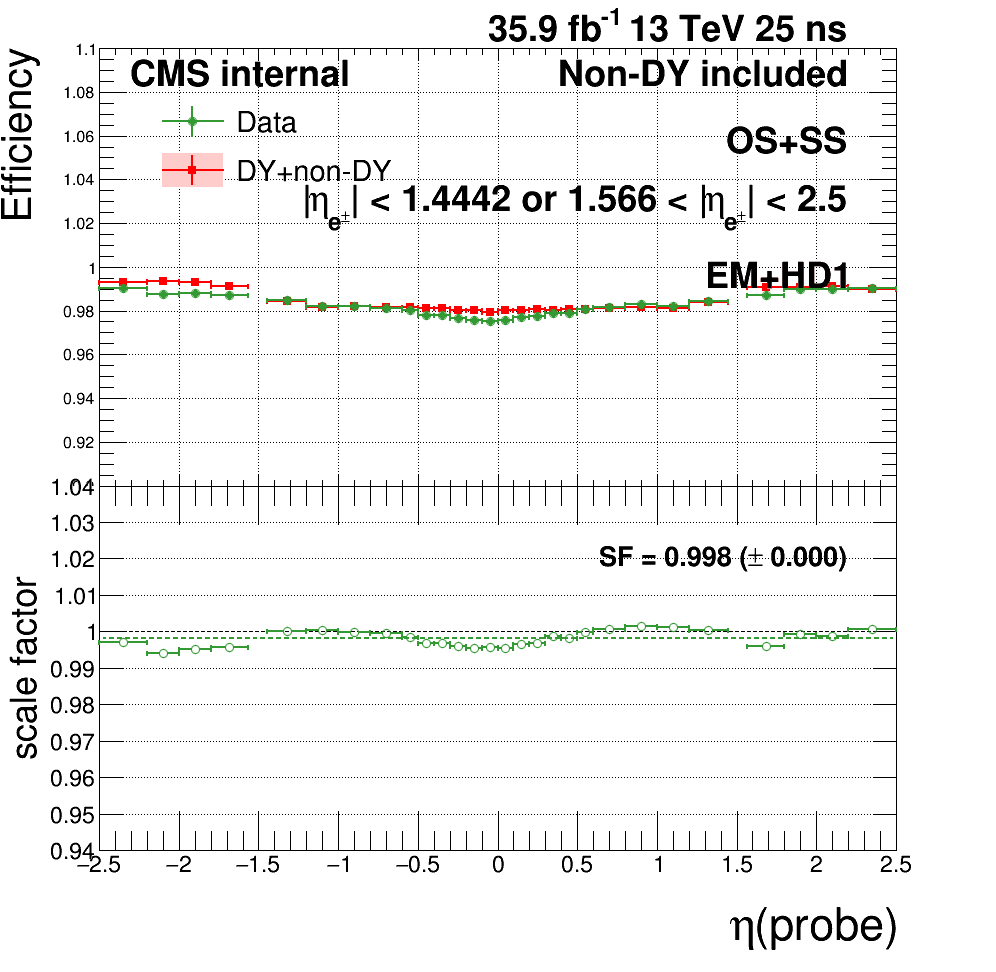
\includegraphics[width=0.45\textwidth]{figures/Zprime/2016/ScaleFactor/SameSign/N_1_eff/g_compare_cut_eta_Barrel+Endcap_ea_ta_inc_AS_N_1_EMHD1Iso_PUW.png}
    \end{tabular}
    \caption{$EM+HD1$ N-1 efficiencies and scale factors in MC and data in the barrel (left) and endcap (right) as functions of probe $E_T$ (top), $N_{vtx}$ (middle) and probe $\eta$ (bottom).}
    \label{fig:EMHD1Iso_2016}
  \end{center}
\end{figure}

\begin{figure}[bh]
  \begin{center}
    \begin{tabular}{cc}
      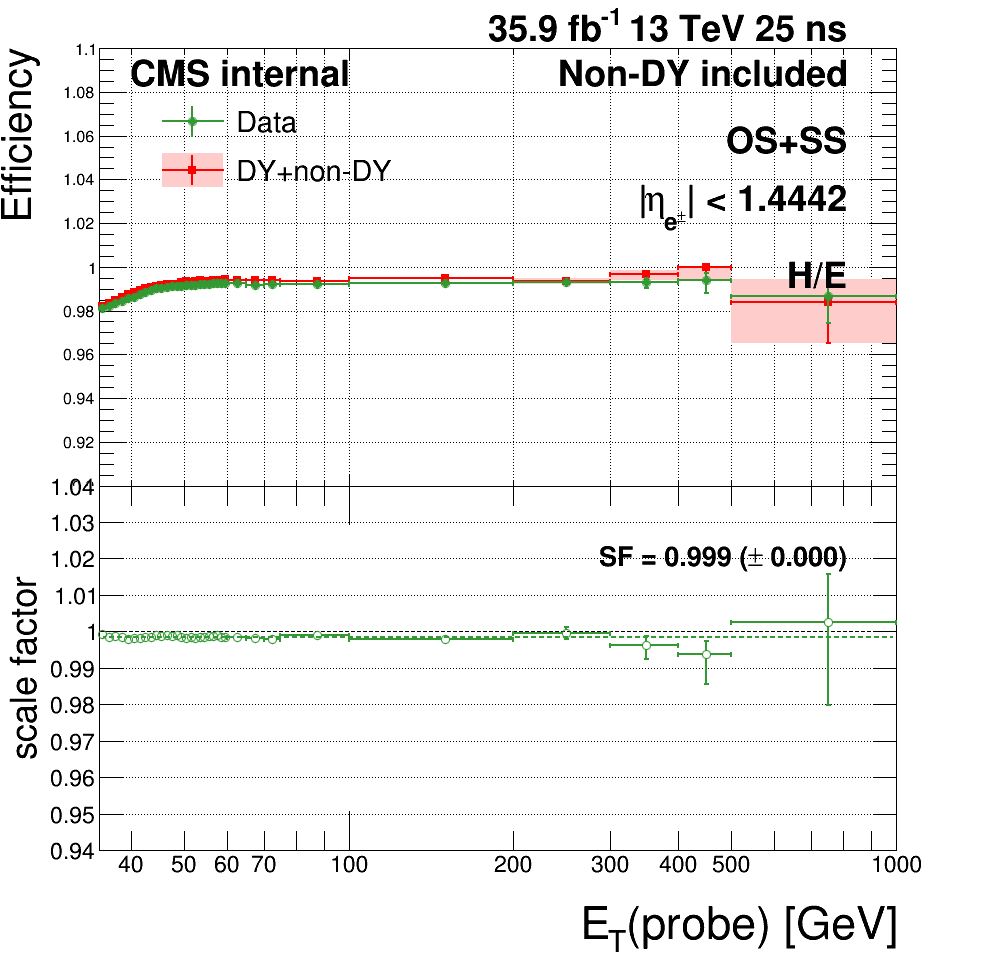
\includegraphics[width=0.45\textwidth]{figures/Zprime/2016/ScaleFactor/SameSign/N_1_eff/g_compare_cut_Et_Barrel_ea_ta_inc_AS_N_1_HoE_PUW.png} &
      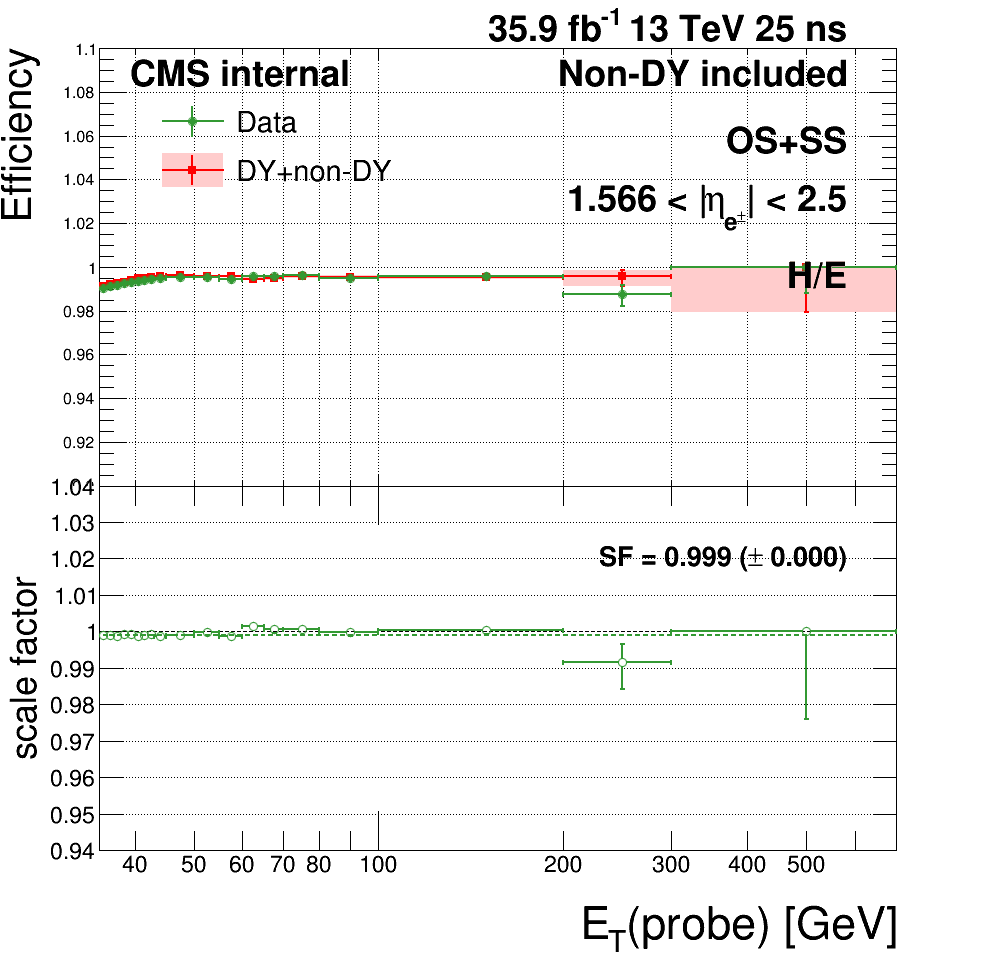
\includegraphics[width=0.45\textwidth]{figures/Zprime/2016/ScaleFactor/SameSign/N_1_eff/g_compare_cut_Et_Endcap_ea_ta_inc_AS_N_1_HoE_PUW.png} \\
      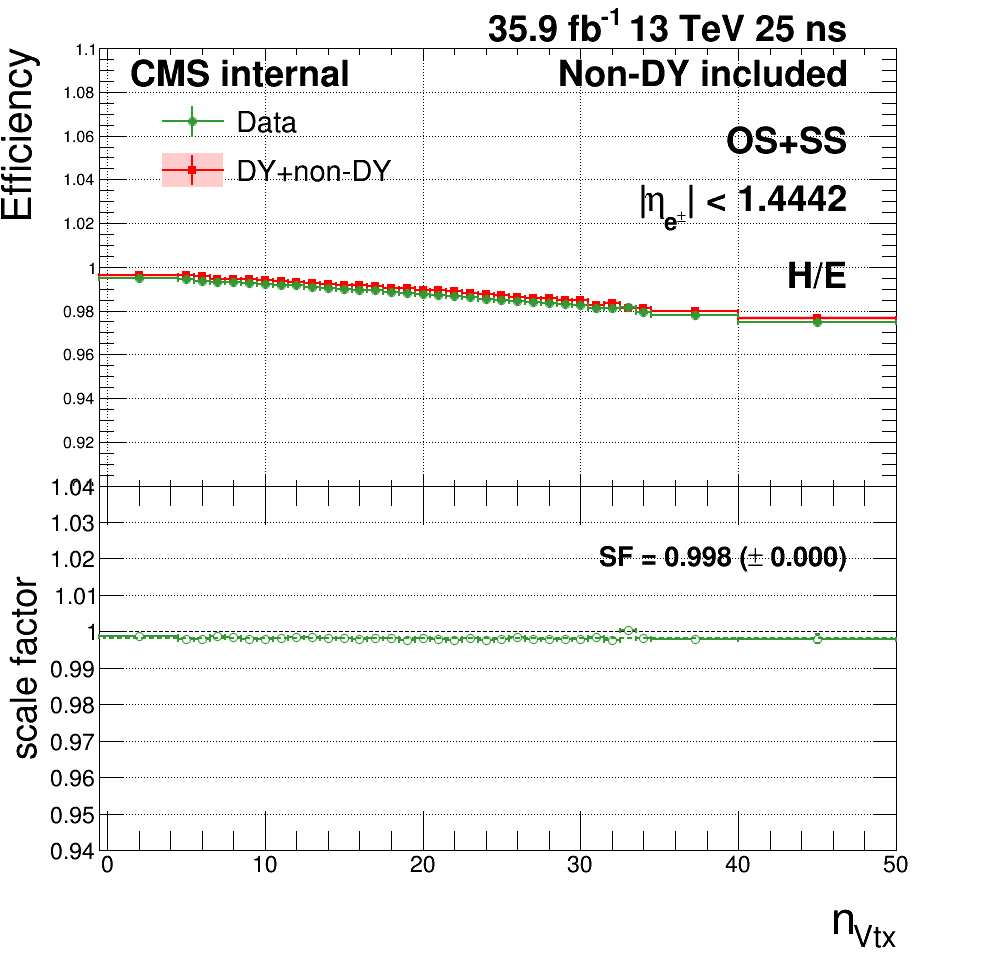
\includegraphics[width=0.45\textwidth]{figures/Zprime/2016/ScaleFactor/SameSign/N_1_eff/g_compare_cut_nVtx_Barrel_ea_ta_inc_AS_N_1_HoE_PUW.png} &
      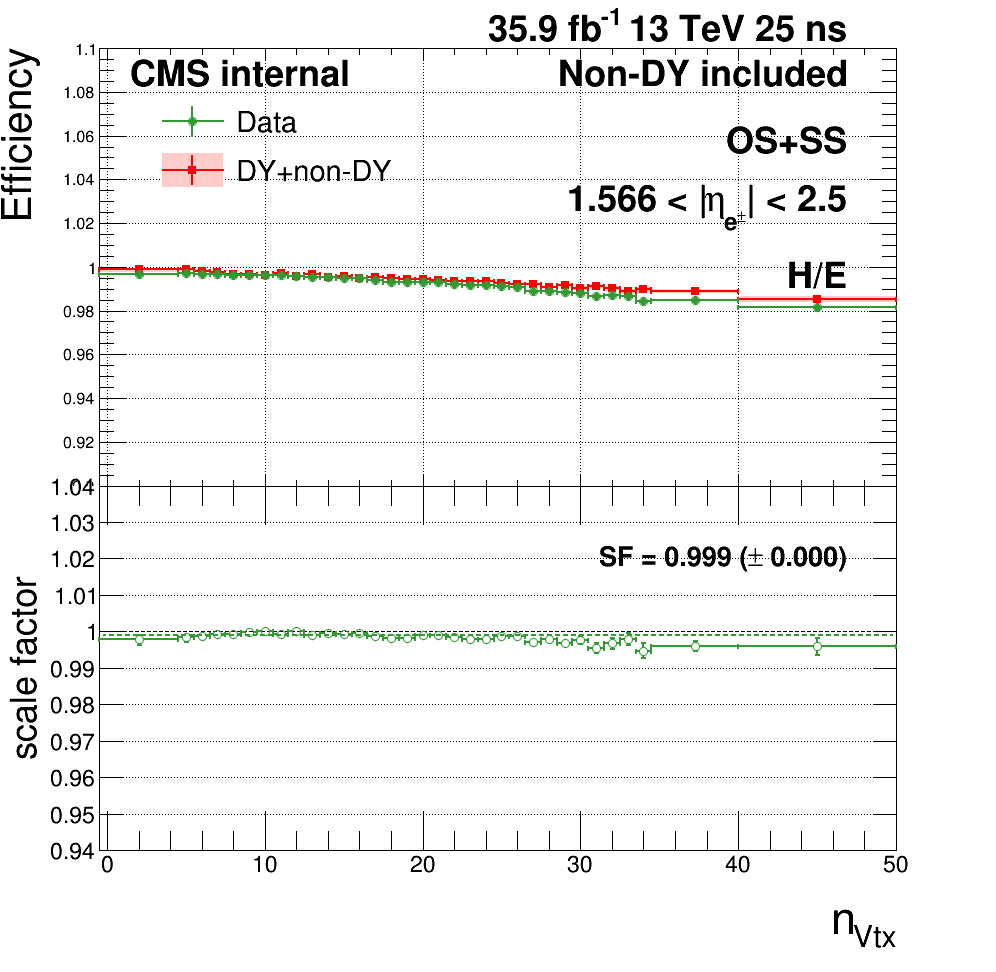
\includegraphics[width=0.45\textwidth]{figures/Zprime/2016/ScaleFactor/SameSign/N_1_eff/g_compare_cut_nVtx_Endcap_ea_ta_inc_AS_N_1_HoE_PUW.png} \\
      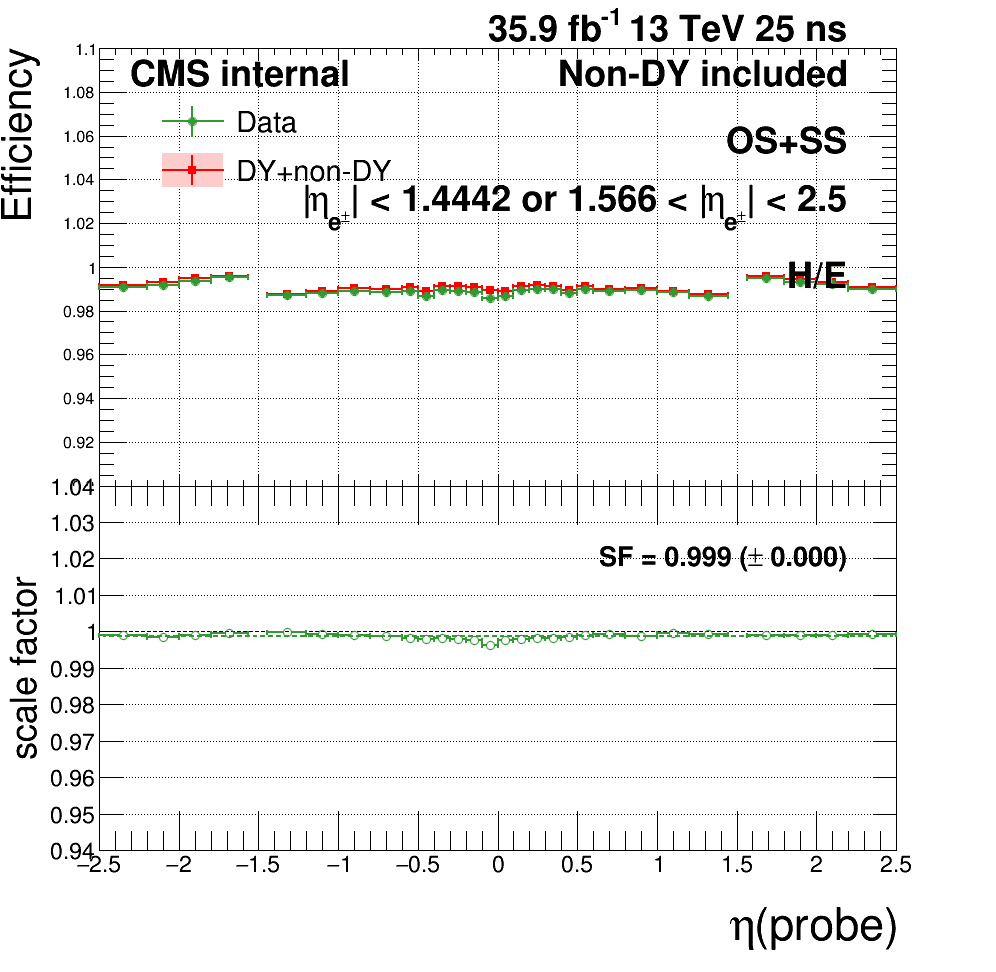
\includegraphics[width=0.45\textwidth]{figures/Zprime/2016/ScaleFactor/SameSign/N_1_eff/g_compare_cut_eta_Barrel+Endcap_ea_ta_inc_AS_N_1_HoE_PUW.png}
    \end{tabular}
    \caption{$H/E$ N-1 efficiencies and scale factors in MC and data in the barrel (left) and endcap (right) as functions of probe $E_T$ (top), $N_{vtx}$ (middle) and probe $\eta$ (bottom).}
    \label{fig:HoE_2016}
  \end{center}
\end{figure}

\begin{figure}[bh]
  \begin{center}
    \begin{tabular}{cc}
      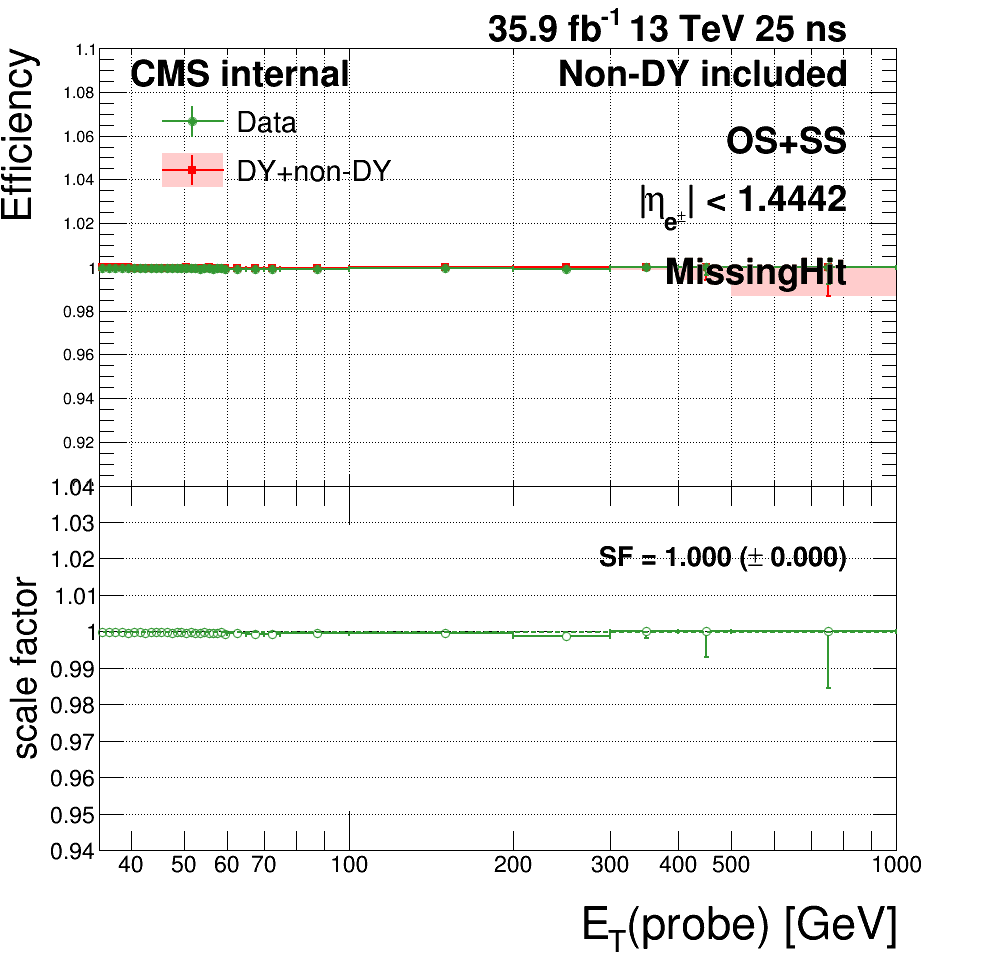
\includegraphics[width=0.45\textwidth]{figures/Zprime/2016/ScaleFactor/SameSign/N_1_eff/g_compare_cut_Et_Barrel_ea_ta_inc_AS_N_1_MissHit_PUW.png} &
      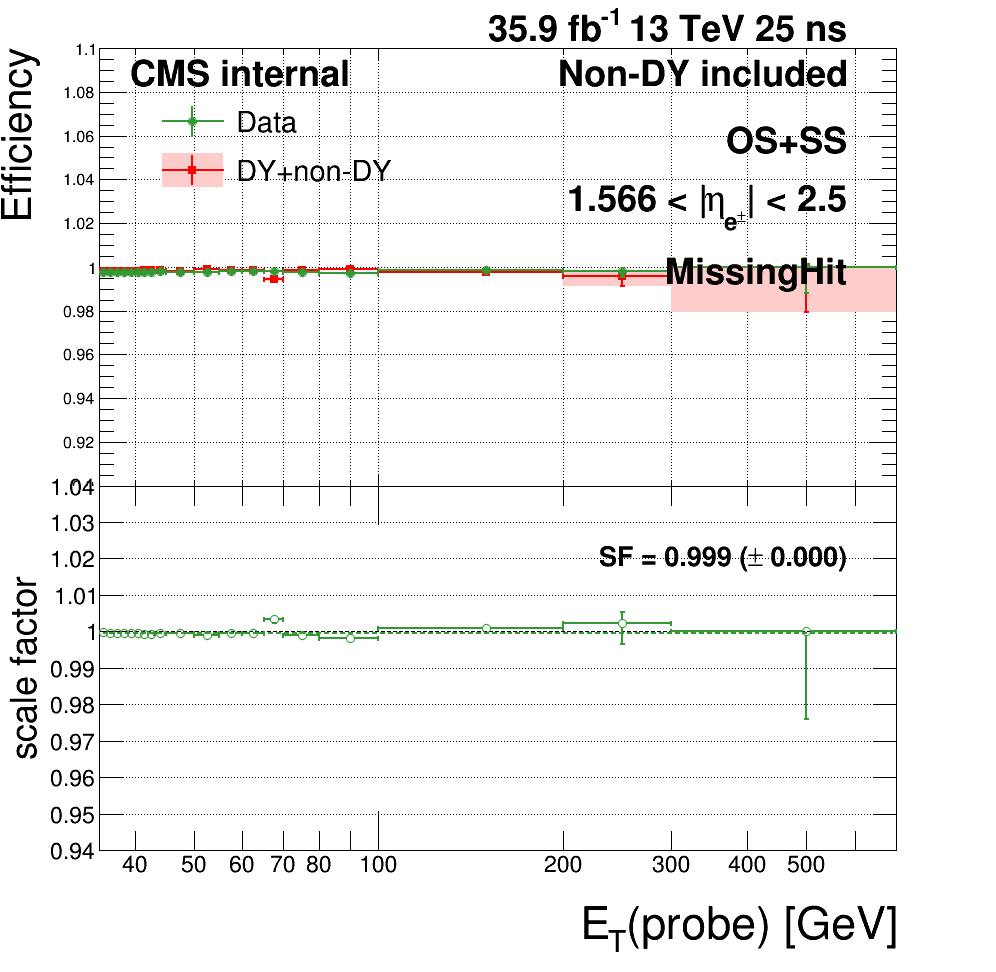
\includegraphics[width=0.45\textwidth]{figures/Zprime/2016/ScaleFactor/SameSign/N_1_eff/g_compare_cut_Et_Endcap_ea_ta_inc_AS_N_1_MissHit_PUW.png} \\
      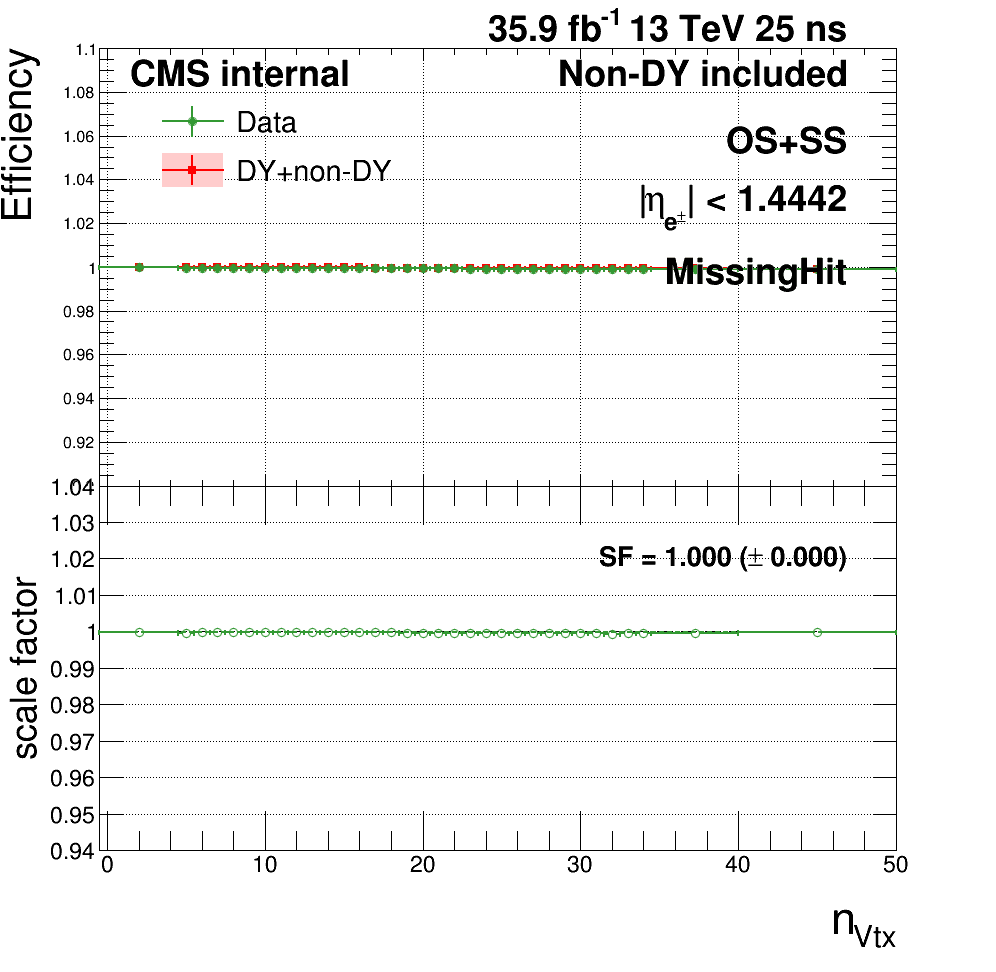
\includegraphics[width=0.45\textwidth]{figures/Zprime/2016/ScaleFactor/SameSign/N_1_eff/g_compare_cut_nVtx_Barrel_ea_ta_inc_AS_N_1_MissHit_PUW.png} &
      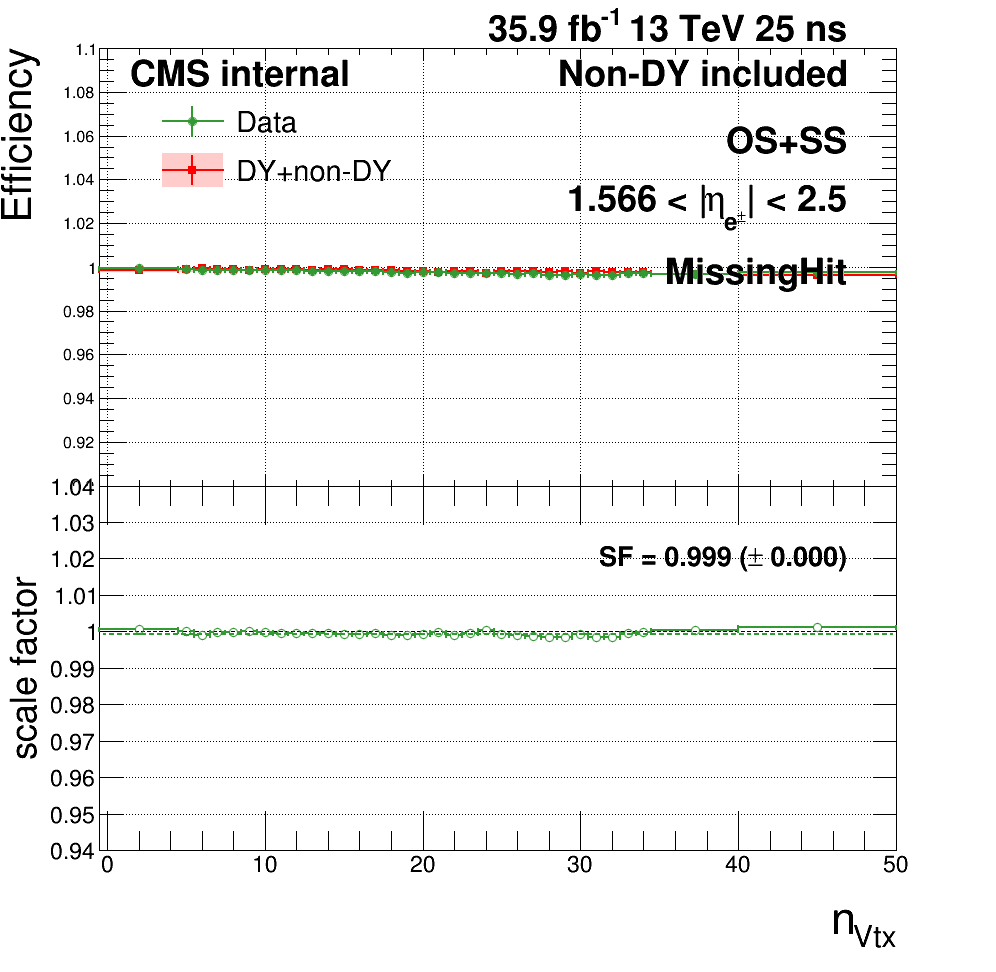
\includegraphics[width=0.45\textwidth]{figures/Zprime/2016/ScaleFactor/SameSign/N_1_eff/g_compare_cut_nVtx_Endcap_ea_ta_inc_AS_N_1_MissHit_PUW.png} \\
      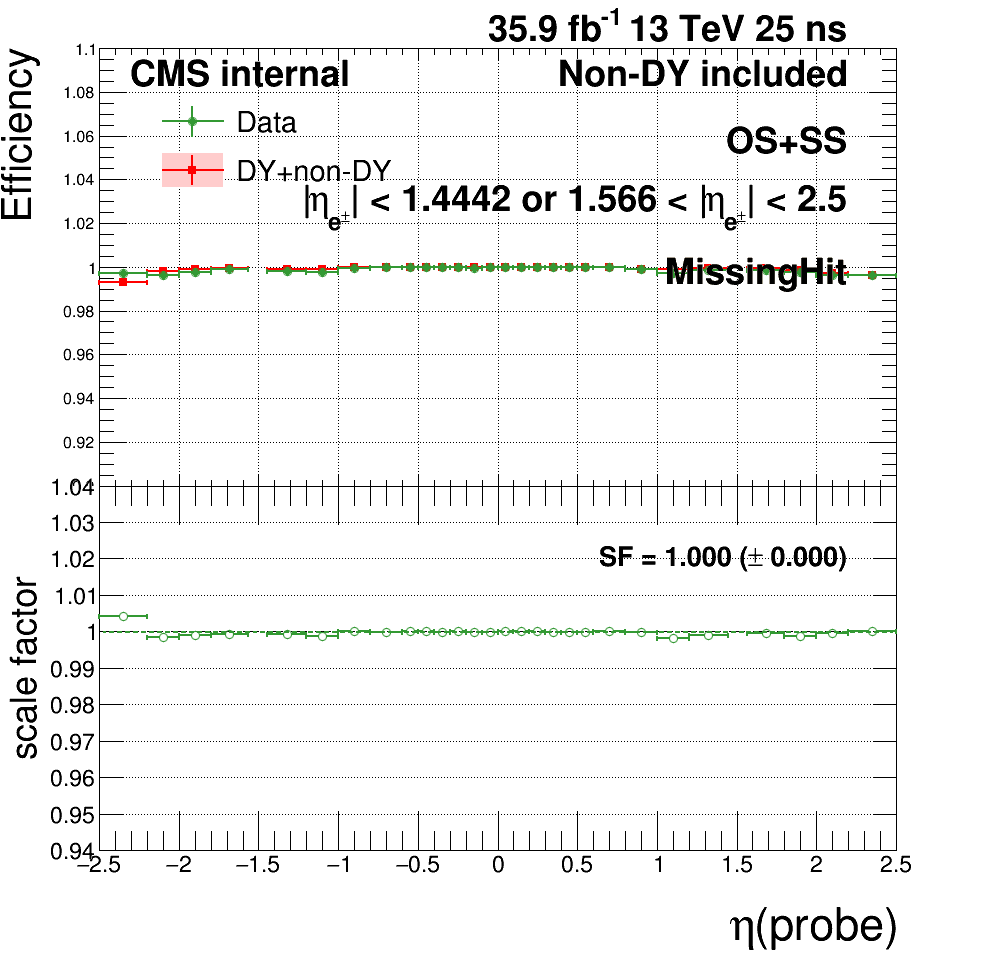
\includegraphics[width=0.45\textwidth]{figures/Zprime/2016/ScaleFactor/SameSign/N_1_eff/g_compare_cut_eta_Barrel+Endcap_ea_ta_inc_AS_N_1_MissHit_PUW.png}
    \end{tabular}
    \caption{$MissingHit$ N-1 efficiencies and scale factors in MC and data in the barrel (left) and endcap (right) as functions of probe $E_T$ (top), $N_{vtx}$ (middle) and probe $\eta$ (bottom).}
    \label{fig:MissHit_2016}
  \end{center}
\end{figure}

\begin{figure}[bh]
  \begin{center}
    \begin{tabular}{cc}
      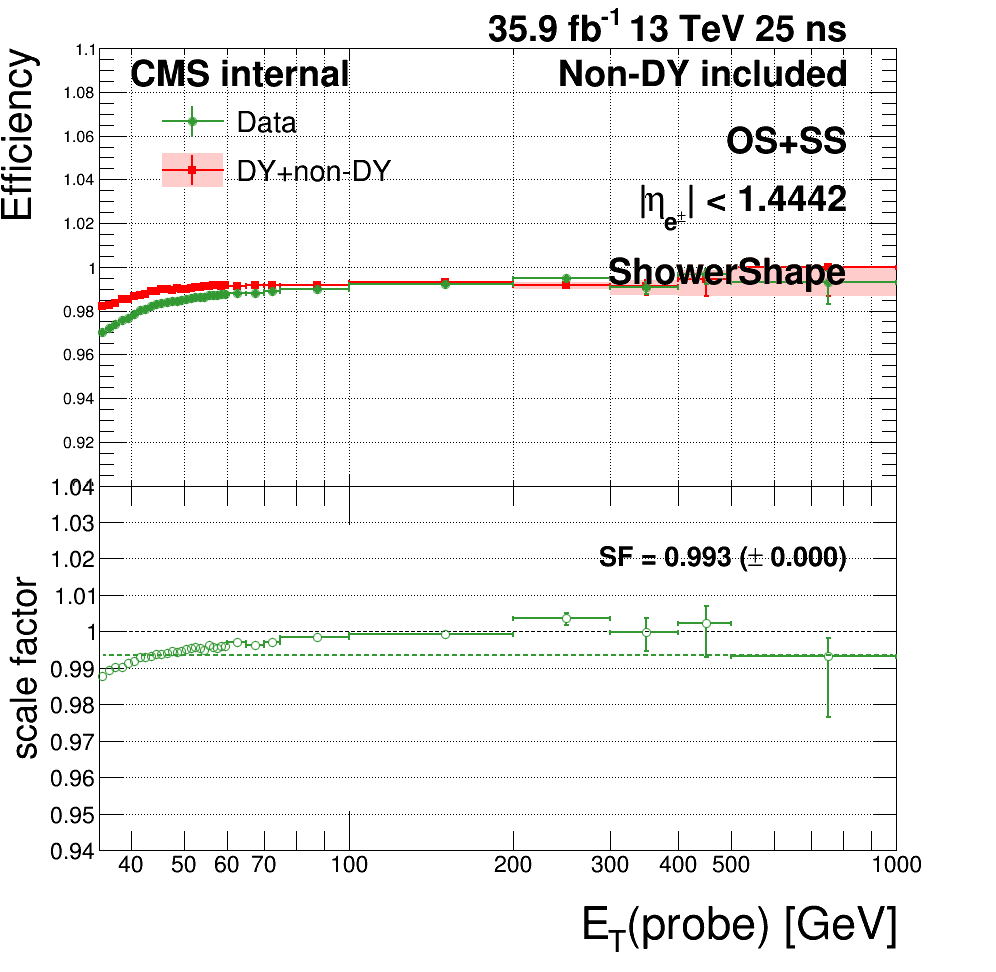
\includegraphics[width=0.45\textwidth]{figures/Zprime/2016/ScaleFactor/SameSign/N_1_eff/g_compare_cut_Et_Barrel_ea_ta_inc_AS_N_1_Shower_PUW.png} &
      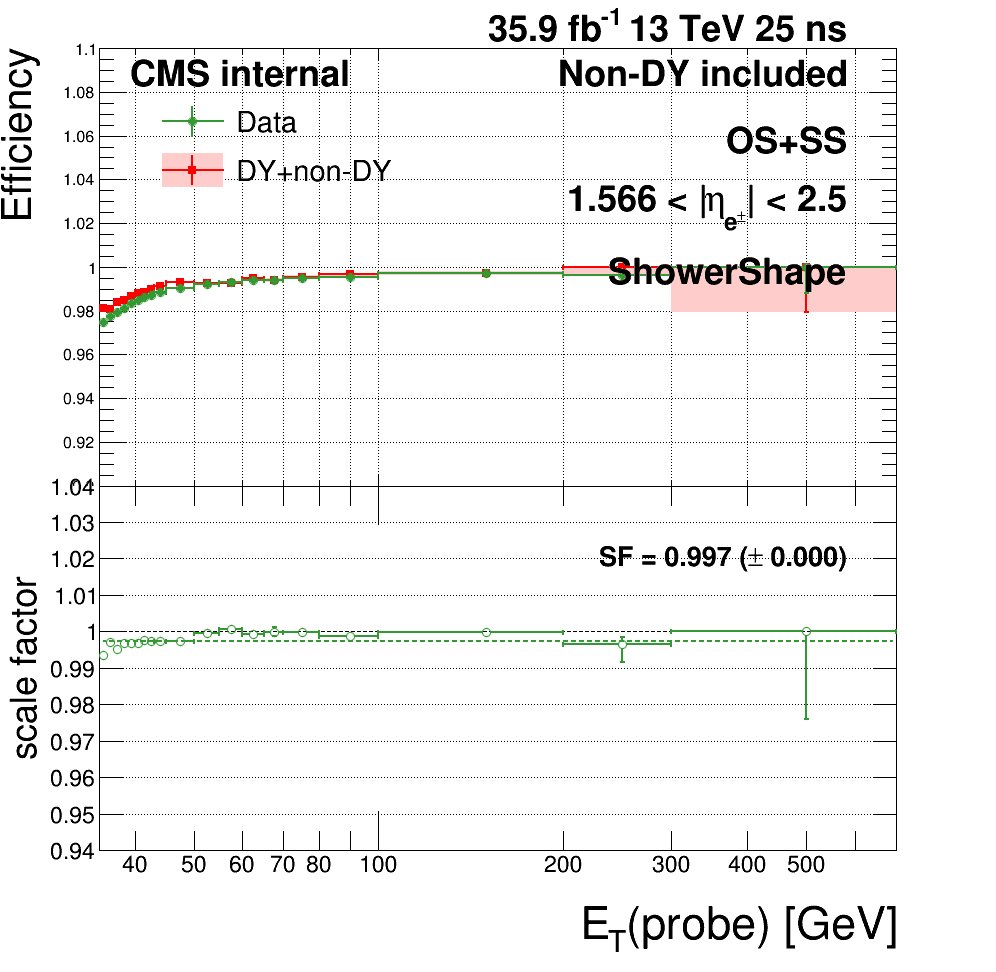
\includegraphics[width=0.45\textwidth]{figures/Zprime/2016/ScaleFactor/SameSign/N_1_eff/g_compare_cut_Et_Endcap_ea_ta_inc_AS_N_1_Shower_PUW.png} \\
      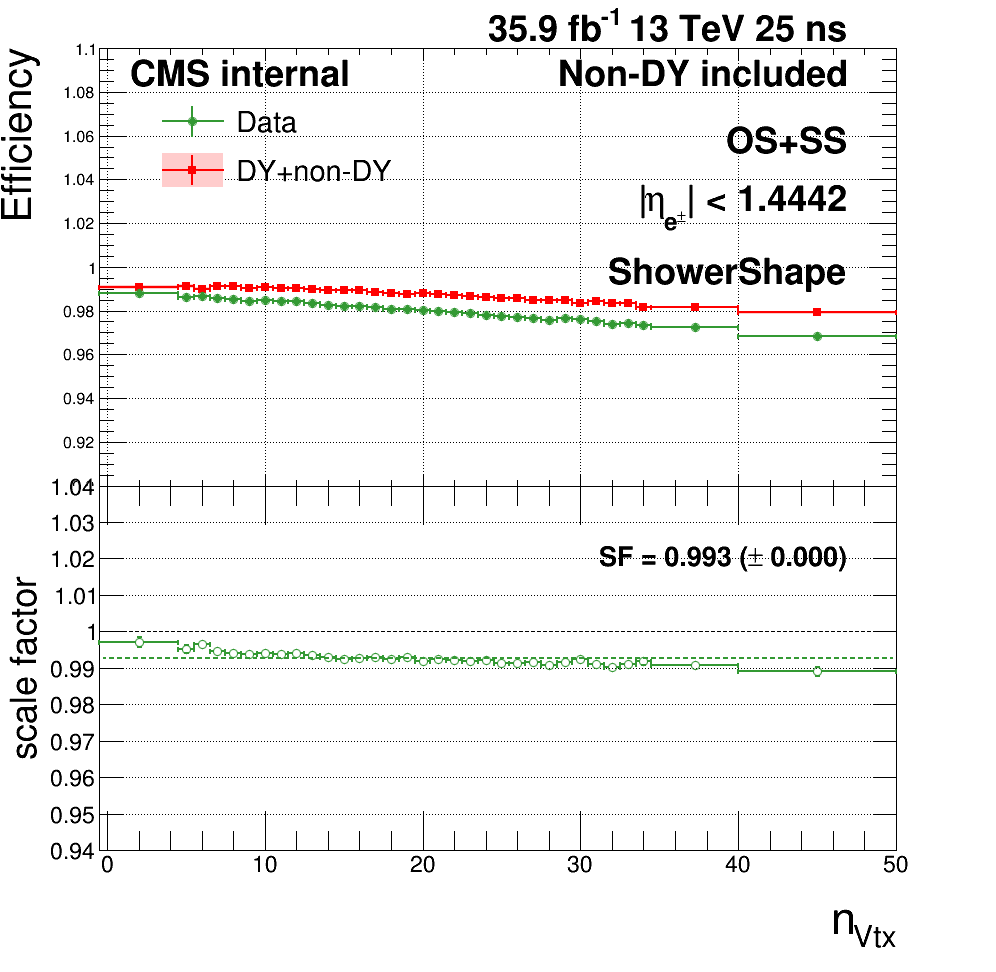
\includegraphics[width=0.45\textwidth]{figures/Zprime/2016/ScaleFactor/SameSign/N_1_eff/g_compare_cut_nVtx_Barrel_ea_ta_inc_AS_N_1_Shower_PUW.png} &
      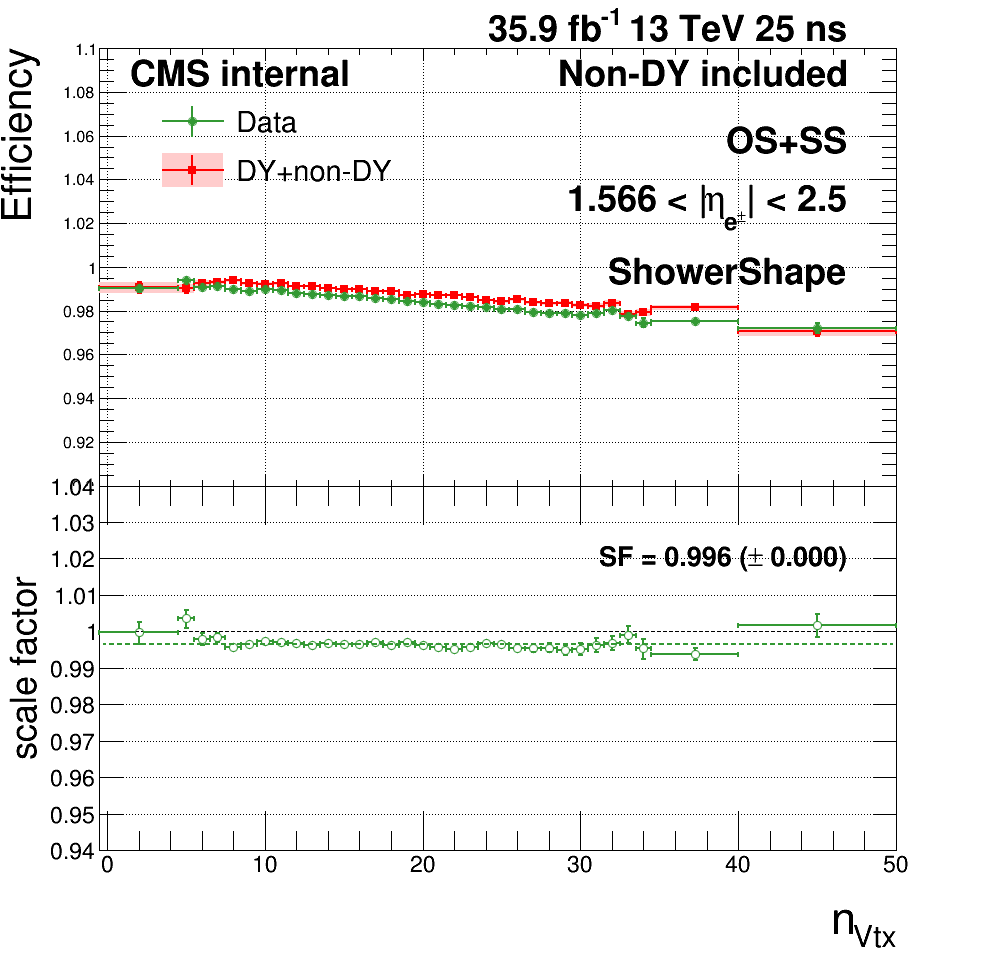
\includegraphics[width=0.45\textwidth]{figures/Zprime/2016/ScaleFactor/SameSign/N_1_eff/g_compare_cut_nVtx_Endcap_ea_ta_inc_AS_N_1_Shower_PUW.png} \\
      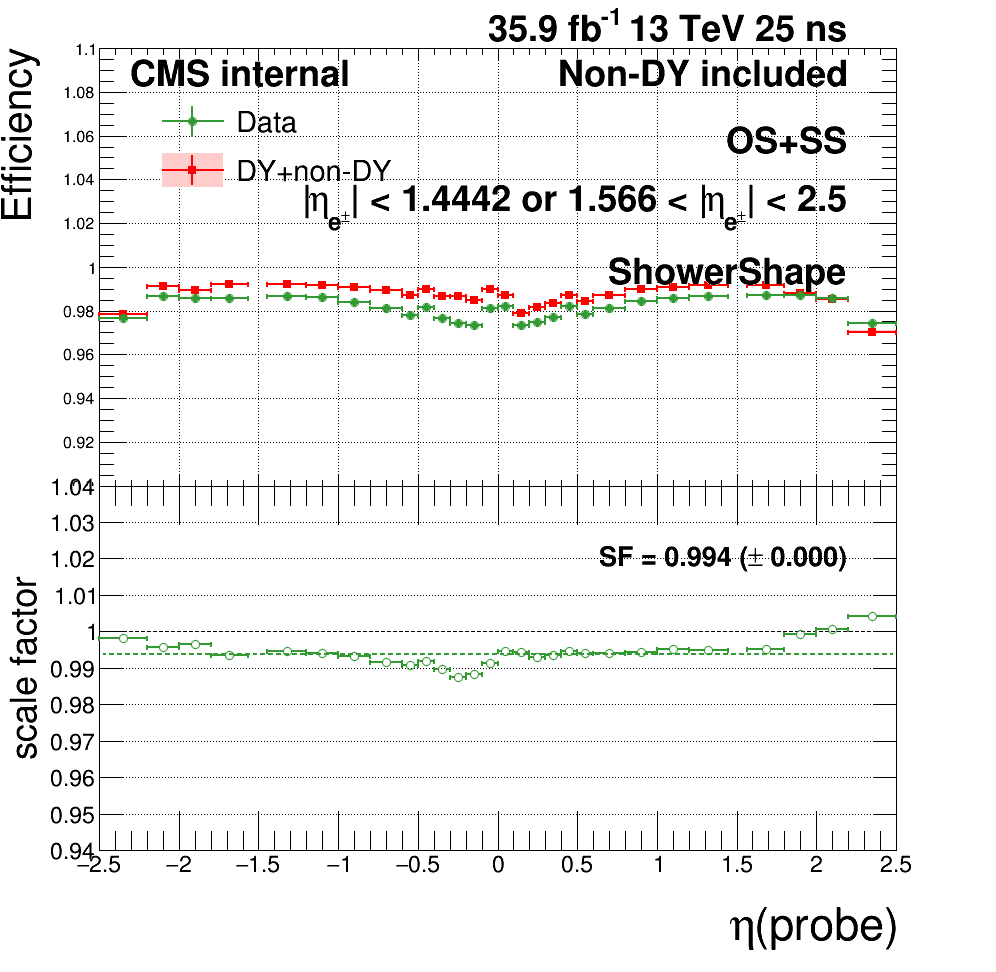
\includegraphics[width=0.45\textwidth]{figures/Zprime/2016/ScaleFactor/SameSign/N_1_eff/g_compare_cut_eta_Barrel+Endcap_ea_ta_inc_AS_N_1_Shower_PUW.png}
    \end{tabular}
    \caption{$ShowerShape$ N-1 efficiencies and scale factors in MC and data in the barrel (left) and endcap (right) as functions of probe $E_T$ (top), $N_{vtx}$ (middle) and probe $\eta$ (bottom).}
    \label{fig:Shower_2016}
  \end{center}
\end{figure}


\begin{figure}[bh]
  \begin{center}
    \begin{tabular}{cc}
      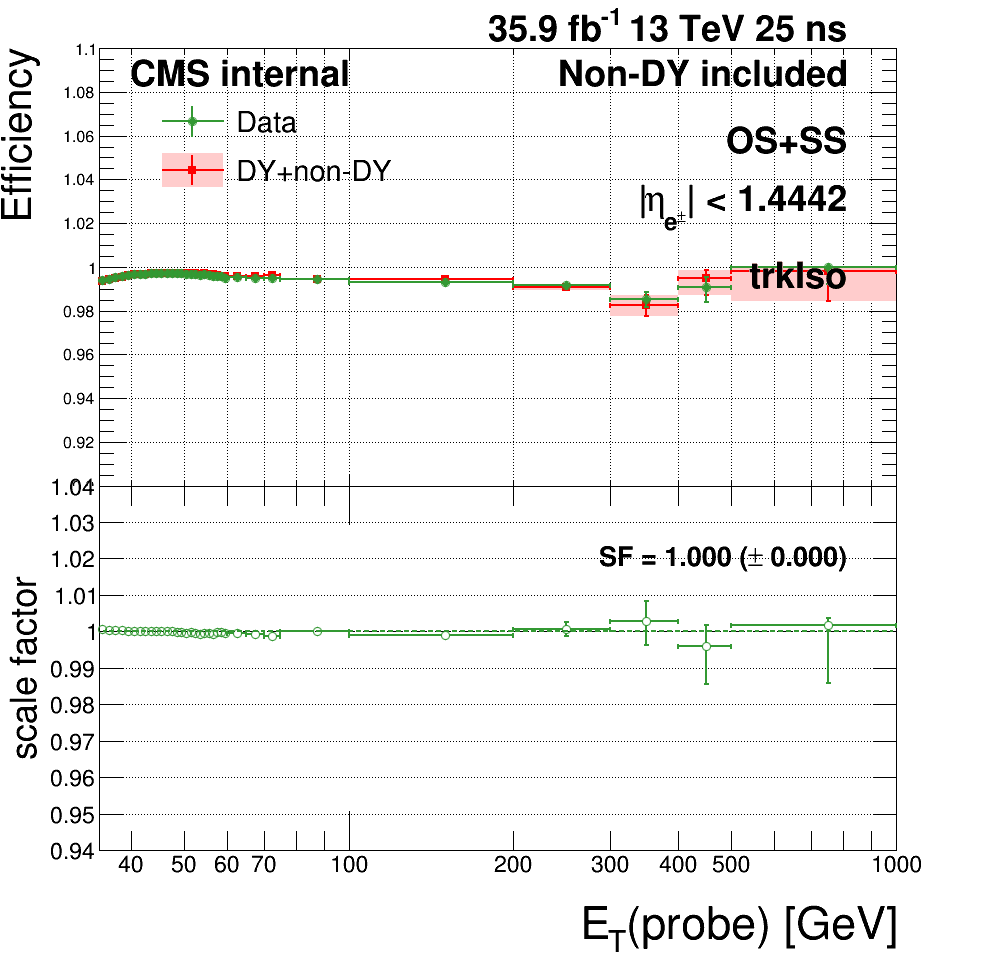
\includegraphics[width=0.45\textwidth]{figures/Zprime/2016/ScaleFactor/SameSign/N_1_eff/g_compare_cut_Et_Barrel_ea_ta_inc_AS_N_1_TrkIso_PUW.png} &
      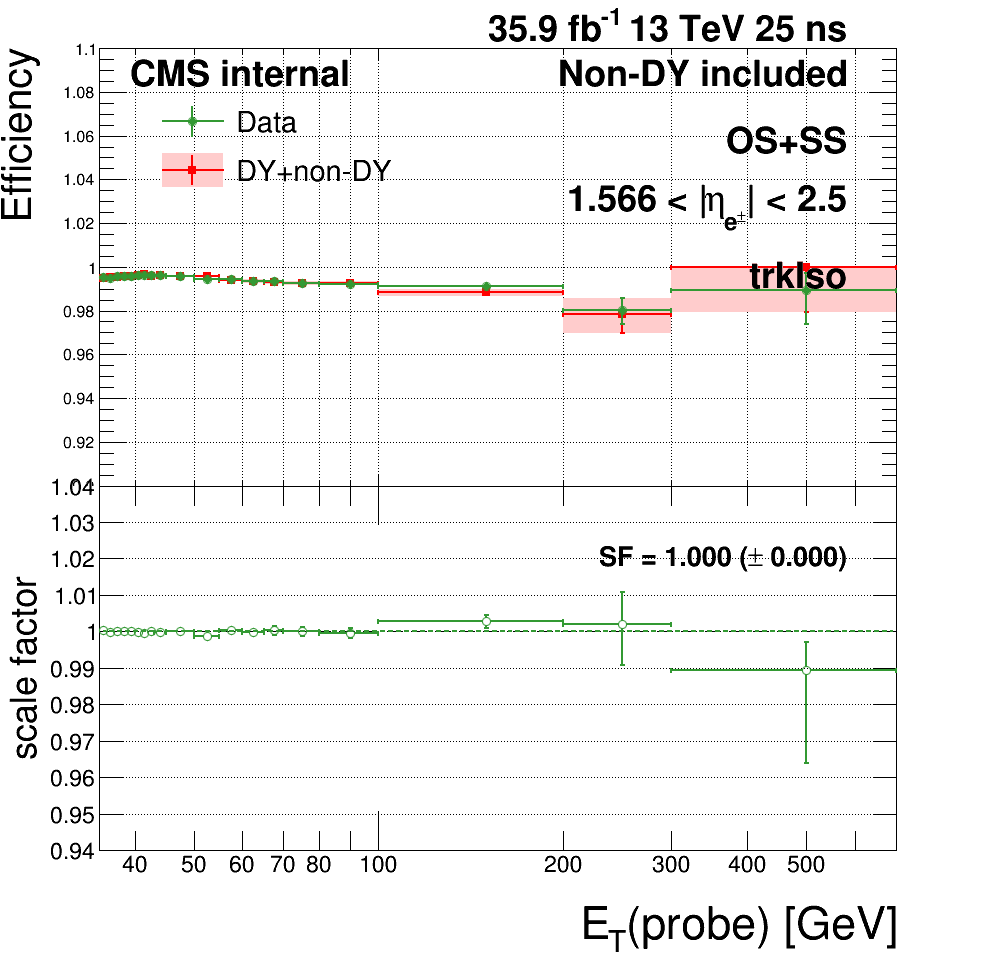
\includegraphics[width=0.45\textwidth]{figures/Zprime/2016/ScaleFactor/SameSign/N_1_eff/g_compare_cut_Et_Endcap_ea_ta_inc_AS_N_1_TrkIso_PUW.png} \\
      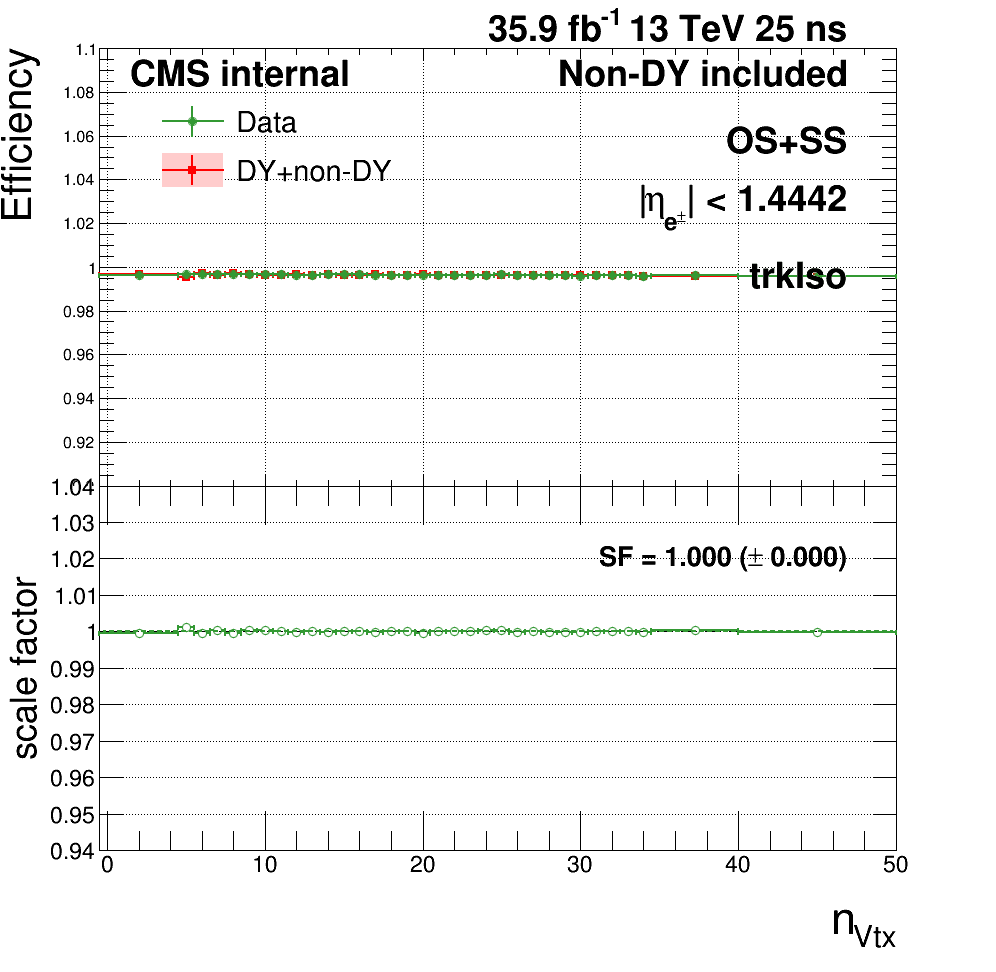
\includegraphics[width=0.45\textwidth]{figures/Zprime/2016/ScaleFactor/SameSign/N_1_eff/g_compare_cut_nVtx_Barrel_ea_ta_inc_AS_N_1_TrkIso_PUW.png} &
      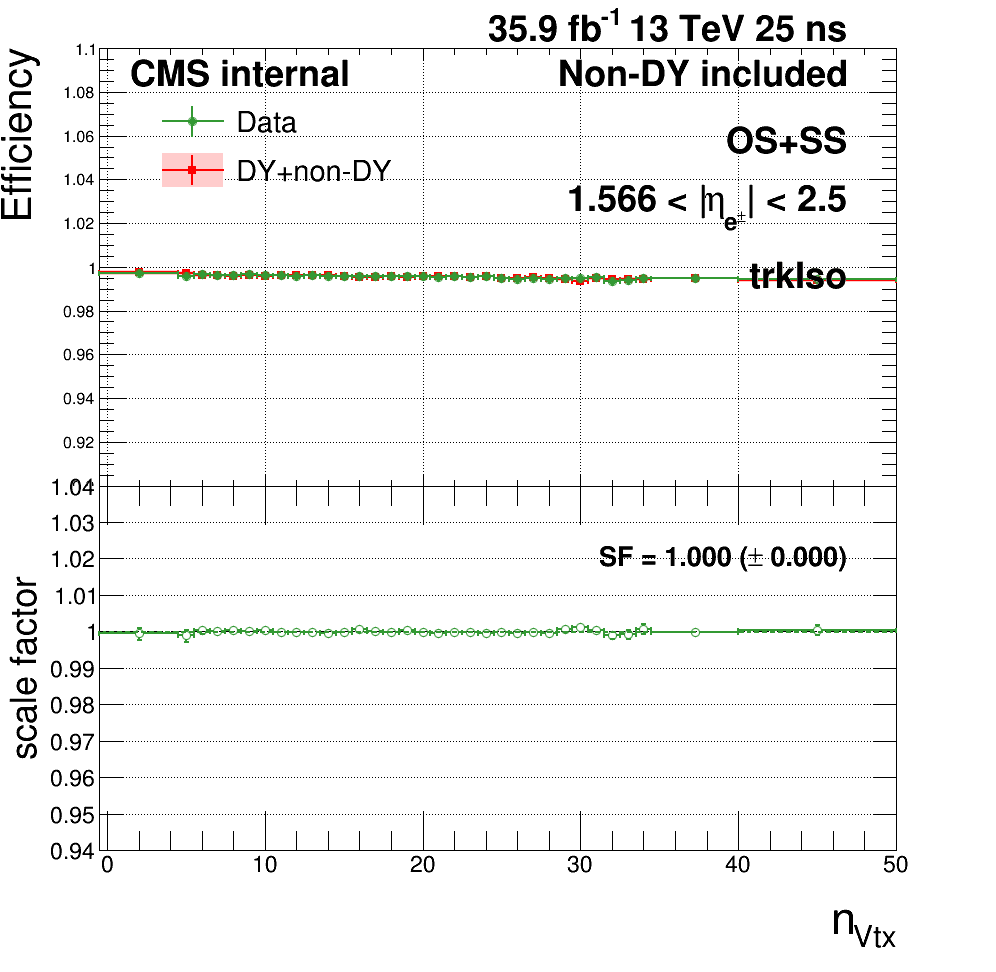
\includegraphics[width=0.45\textwidth]{figures/Zprime/2016/ScaleFactor/SameSign/N_1_eff/g_compare_cut_nVtx_Endcap_ea_ta_inc_AS_N_1_TrkIso_PUW.png} \\
      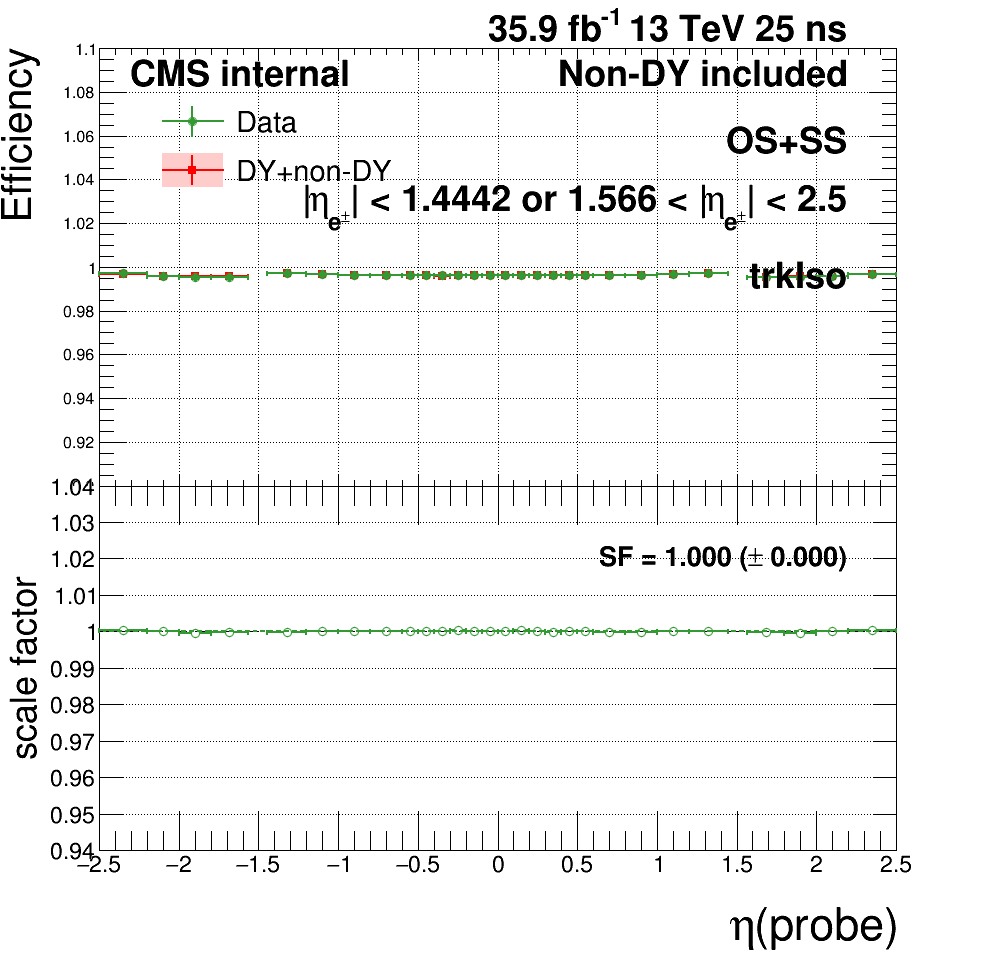
\includegraphics[width=0.45\textwidth]{figures/Zprime/2016/ScaleFactor/SameSign/N_1_eff/g_compare_cut_eta_Barrel+Endcap_ea_ta_inc_AS_N_1_TrkIso_PUW.png}
    \end{tabular}
    \caption{$track isolation$ N-1 efficiencies and scale factors in MC and data in the barrel (left) and endcap (right) as functions of probe $E_T$ (top), $N_{vtx}$ (middle) and probe $\eta$ (bottom).}
    \label{fig:TrkIso_2016}
  \end{center}
\end{figure}

\clearpage
\begin{figure}[bh]
  \begin{center}
    \begin{tabular}{cc}
      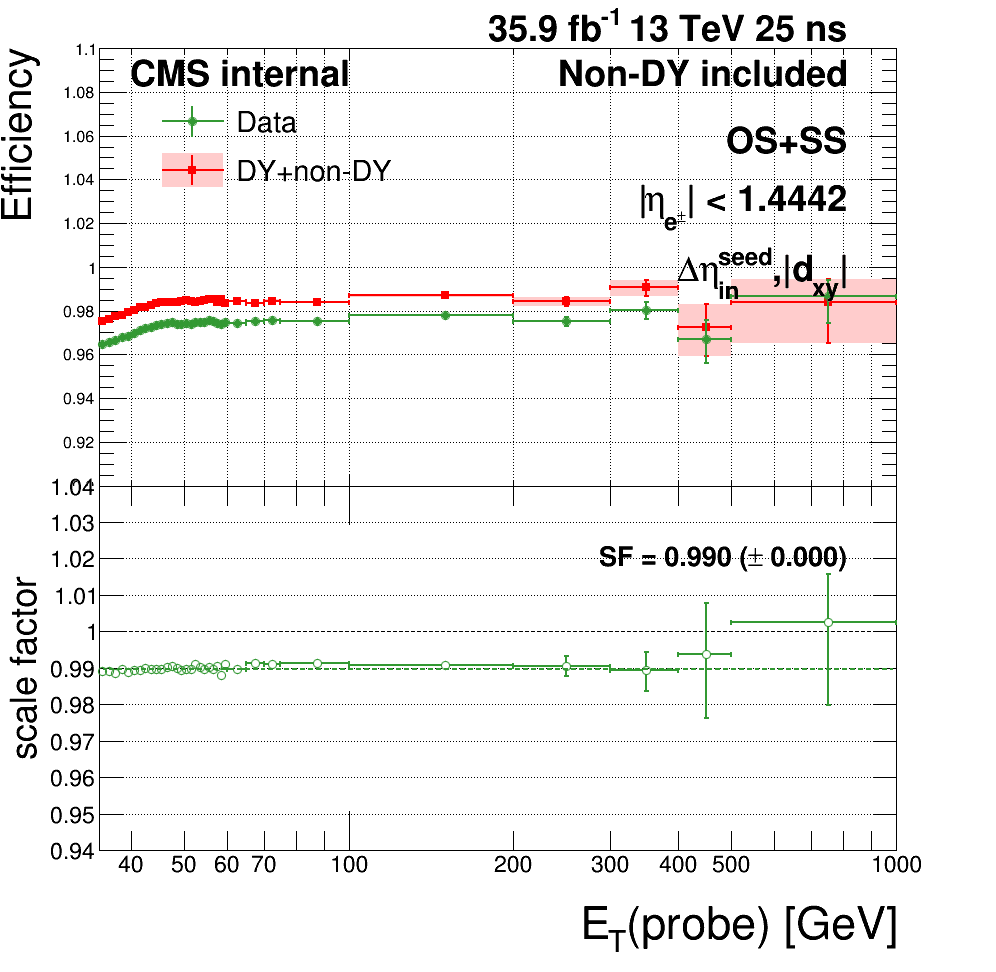
\includegraphics[width=0.45\textwidth]{figures/Zprime/2016/ScaleFactor/SameSign/N_1_eff/g_compare_cut_Et_Barrel_ea_ta_inc_AS_N_2_DetaIn_Dxy_PUW.png} &
      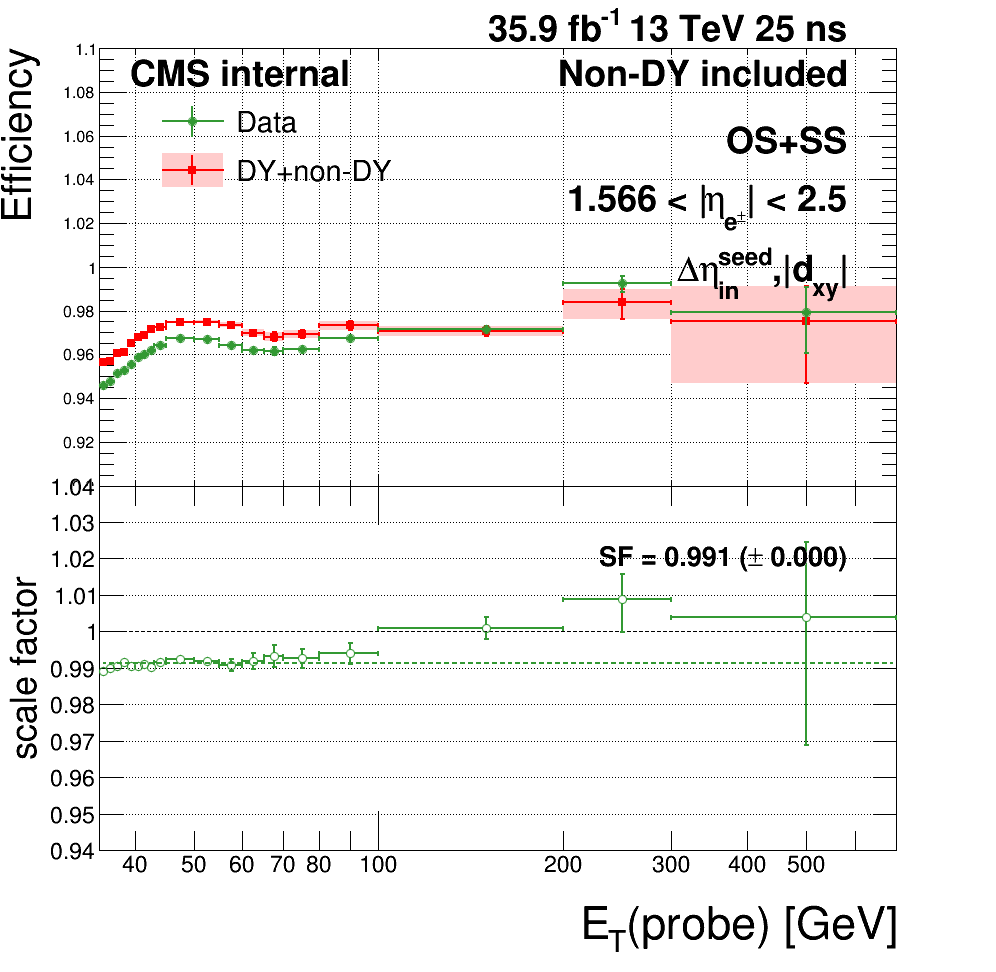
\includegraphics[width=0.45\textwidth]{figures/Zprime/2016/ScaleFactor/SameSign/N_1_eff/g_compare_cut_Et_Endcap_ea_ta_inc_AS_N_2_DetaIn_Dxy_PUW.png} \\
      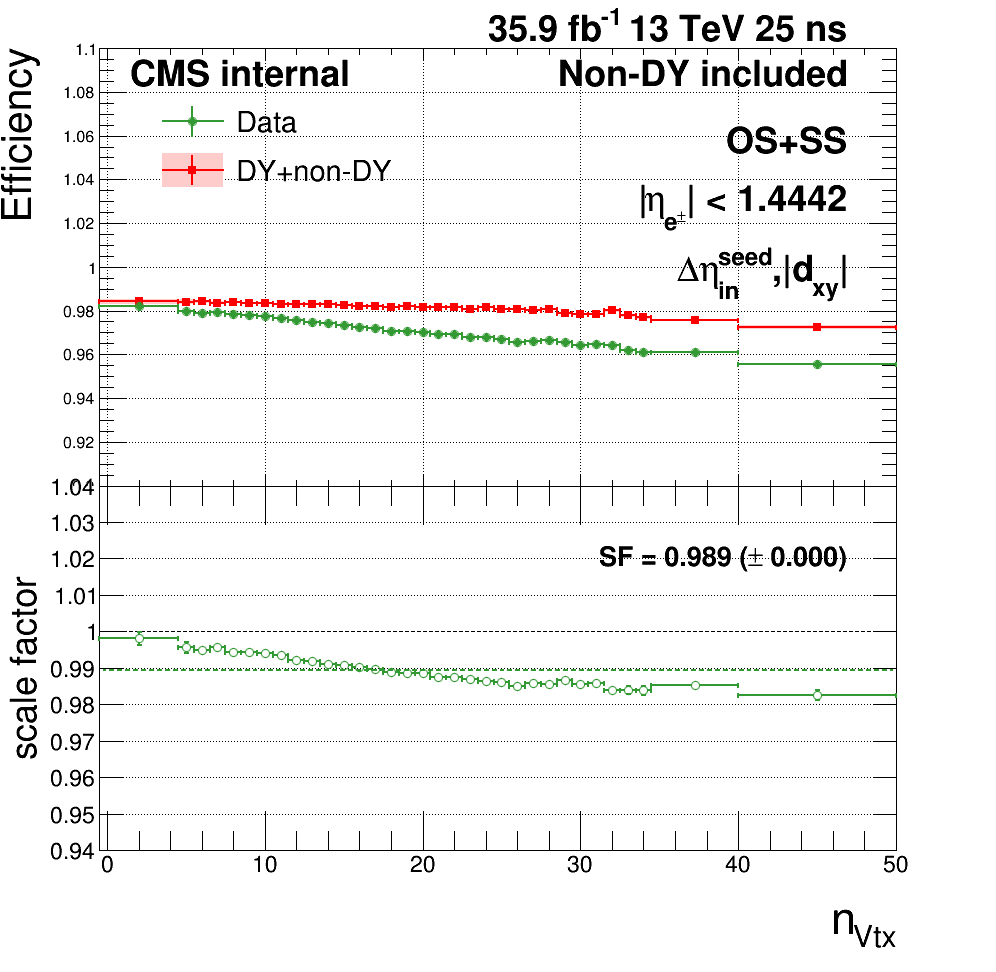
\includegraphics[width=0.45\textwidth]{figures/Zprime/2016/ScaleFactor/SameSign/N_1_eff/g_compare_cut_nVtx_Barrel_ea_ta_inc_AS_N_2_DetaIn_Dxy_PUW.png} &
      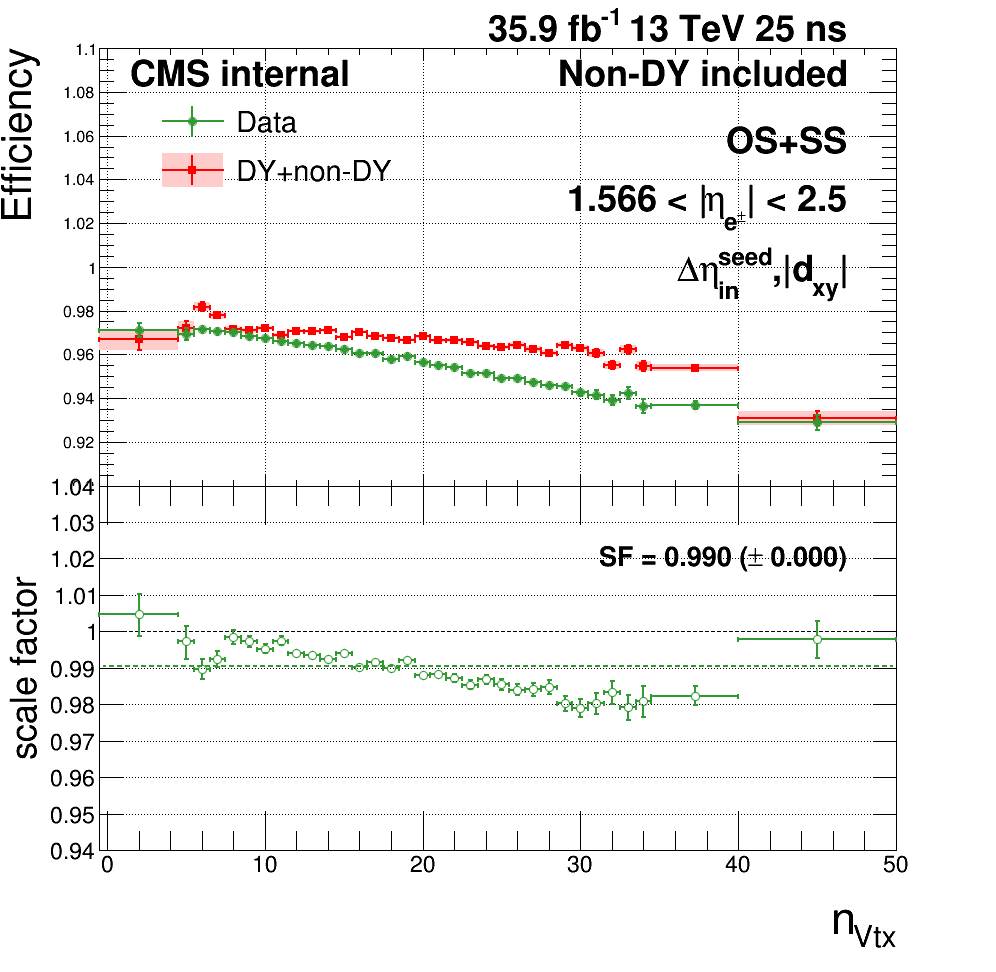
\includegraphics[width=0.45\textwidth]{figures/Zprime/2016/ScaleFactor/SameSign/N_1_eff/g_compare_cut_nVtx_Endcap_ea_ta_inc_AS_N_2_DetaIn_Dxy_PUW.png} \\
      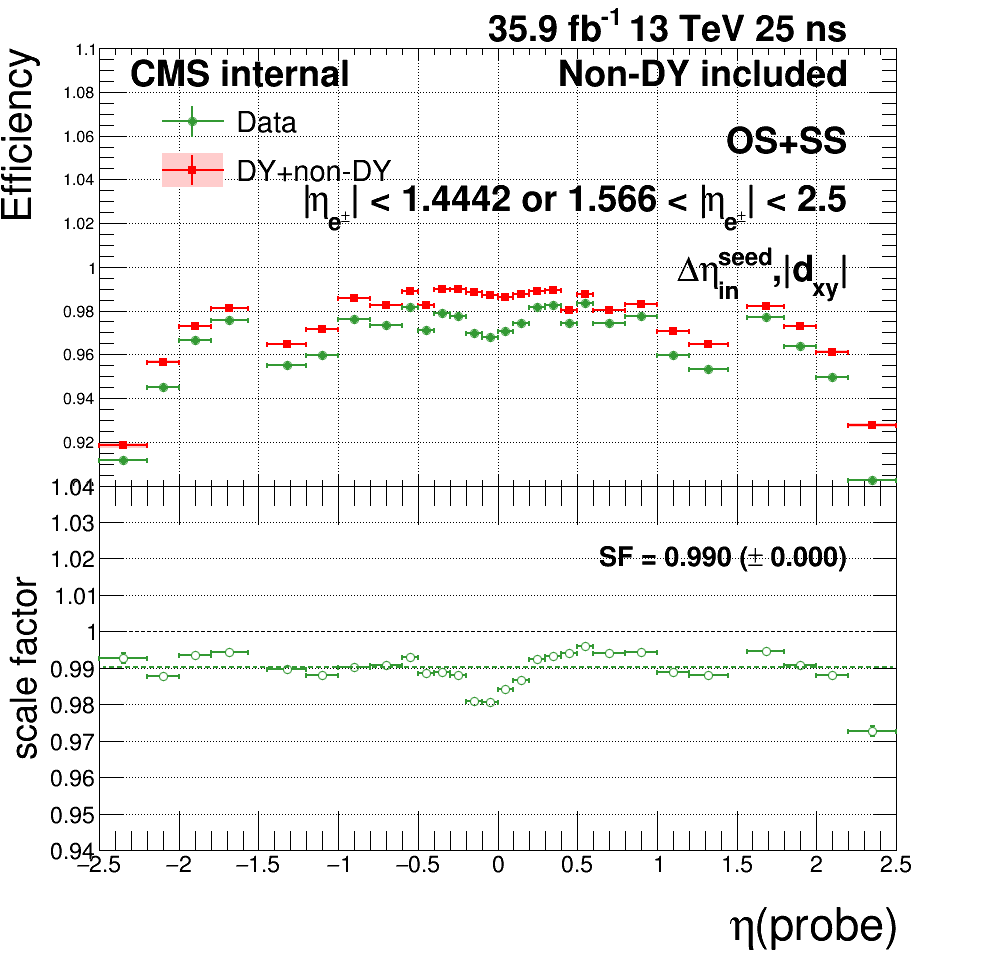
\includegraphics[width=0.45\textwidth]{figures/Zprime/2016/ScaleFactor/SameSign/N_1_eff/g_compare_cut_eta_Barrel+Endcap_ea_ta_inc_AS_N_2_DetaIn_Dxy_PUW.png}
    \end{tabular}
    \caption{$\Delta \eta_{in}^{seed}$ and $|d_{xy}|$ N-2 efficiencies and scale factors in MC and data in the barrel (left) and endcap (right) as functions of probe $E_T$ (top), $N_{vtx}$ (middle) and probe $\eta$ (bottom).}
    \label{fig:DetaIn_Dxy_2016}
  \end{center}
\end{figure}

\begin{figure}[bh]
  \begin{center}
    \begin{tabular}{cc}
      \includegraphics[width=0.45\textwidth]{figures/Zprime/2016/ScaleFactor/SameSign/N_1_eff/g_compare_cut_Et_Barrel_ea_ta_inc_AS_N_3_Trk_PUW.png} &
      \includegraphics[width=0.45\textwidth]{figures/Zprime/2016/ScaleFactor/SameSign/N_1_eff/g_compare_cut_Et_Endcap_ea_ta_inc_AS_N_3_Trk_PUW.png} \\
      \includegraphics[width=0.45\textwidth]{figures/Zprime/2016/ScaleFactor/SameSign/N_1_eff/g_compare_cut_nVtx_Barrel_ea_ta_inc_AS_N_3_Trk_PUW.png} &
      \includegraphics[width=0.45\textwidth]{figures/Zprime/2016/ScaleFactor/SameSign/N_1_eff/g_compare_cut_nVtx_Endcap_ea_ta_inc_AS_N_3_Trk_PUW.png} \\
      \includegraphics[width=0.45\textwidth]{figures/Zprime/2016/ScaleFactor/SameSign/N_1_eff/g_compare_cut_eta_Barrel+Endcap_ea_ta_inc_AS_N_3_Trk_PUW.png}
    \end{tabular}
    \caption{$\Delta \eta_{in}^{seed}$, $|d_{xy}|$ and $\Delta \phi_{in}$ N-3 efficiencies and scale factors in MC and data in the barrel (left) and endcap (right) as functions of probe $E_T$ (top), $N_{vtx}$ (middle) and probe $\eta$ (bottom).}
    \label{fig:DetaIn_Dxy_DphiIn_2016}
  \end{center}
\end{figure}

\clearpage
\subsection{HEEP efficiency versus \texorpdfstring{$\eta$}{h1} for different \texorpdfstring{$\et$}{h2} bins}
\label{AppHEEPsf_eta_Et_bins_2016}
As can be seen in Figure \ref{fig:eff_SS_nominal_eta_2016}, scale factor drops by 2-3\% around $|\eta|=0$.
The efficiencies and scale factors are shown as functions of $\eta$ for $\et$ of probe from $35-50 (~\mathrm{GeV})$, $50-100 (~\mathrm{GeV})$ and $>100 (~\mathrm{GeV})$ in Figure \ref{fig:eta_Et_bins_2016}. One can see the behaviour of scale factor for $\eta$ close to 0 for different $\et$ bins are similar, so it is $\et$ independent.
\begin{figure}[bh]
  \begin{center}
    \begin{tabular}{cc}
      \includegraphics[width=0.45\textwidth]{figures/Zprime/2016/ScaleFactor/SameSign/eta_Et_bins/g_compare_cut_eta_Barrel+Endcap_ea_ta_inc_AS_ProbeEt_35_50_PUW.png} &
      \includegraphics[width=0.45\textwidth]{figures/Zprime/2016/ScaleFactor/SameSign/eta_Et_bins/g_compare_cut_eta_Barrel+Endcap_ea_ta_exc_AS_ProbeEt_35_50_PUW.png} \\
      \includegraphics[width=0.45\textwidth]{figures/Zprime/2016/ScaleFactor/SameSign/eta_Et_bins/g_compare_cut_eta_Barrel+Endcap_ea_ta_inc_AS_ProbeEt_50_100_PUW.png} &
      \includegraphics[width=0.45\textwidth]{figures/Zprime/2016/ScaleFactor/SameSign/eta_Et_bins/g_compare_cut_eta_Barrel+Endcap_ea_ta_exc_AS_ProbeEt_50_100_PUW.png}\\
      \includegraphics[width=0.45\textwidth]{figures/Zprime/2016/ScaleFactor/SameSign/eta_Et_bins/g_compare_cut_eta_Barrel+Endcap_ea_ta_inc_AS_ProbeEt_100_inf_PUW.png} &
      \includegraphics[width=0.45\textwidth]{figures/Zprime/2016/ScaleFactor/SameSign/eta_Et_bins/g_compare_cut_eta_Barrel+Endcap_ea_ta_exc_AS_ProbeEt_100_inf_PUW.png}
    \end{tabular}
    \caption{Efficiencies and scale factors in MC and data for $\et$ of probe bin $35-50 (~\mathrm{GeV})$ (top), $50-100 (~\mathrm{GeV})$ (middle) and $>100 (~\mathrm{GeV})$ (bottom) where the non-DY processes are included (left) and subtracted (right) as functions of probe $\eta$.}
    \label{fig:eta_Et_bins_2016}
  \end{center}
\end{figure}

In addition, HEEP scale factor is measured in three $\eta$ bins and summarized in Table \ref{tab:eff_eta_bins_2016}
\begin{table}[!htbp]
  \caption{\label{tab:eff_eta_bins_2016}
  HEEP scale factors for different $\eta$ bins.}
  \begin{center}
    \tabcolsep=15pt
    \begin{tabular}{ccccccc}
      \hline
      $\eta$        & $-2.5~to~-1.566$         & $-1.4442~to~-0.5$       & $-0.5~to~0$            \\
      \hline
      Scale factor  & $0.985 \pm 0.001(stat.)$ & $0.971\pm 0.001(stat.)$ & $0.961\pm 0.001(stat.)$ \\
      \hline
      \hline
      $\eta$        & $0~to~0.5$                & $0.5~to~1.4442$         & $1.566~to~2.5$ \\
      \hline
      Scale factor  & $0.974\pm 0.001(stat.)$ & $0.978\pm 0.001(stat.)$ & $0.982\pm 0.002(stat.)$ \\
      \hline
    \end{tabular}
  \end{center}
\end{table}

\clearpage
%\section{HEEP efficiency for different runs}
%\label{AppHEEPsf_diffRuns}
%In Figure \ref{fig:RunB2F} and \ref{fig:RunGH}, HEEP efficinecy is shown for runs B-F (with ``HIP'' problem) and runs G-H (without ``HIP'' problem), respectively. Comparing HEEP efficiency versus number of vertice for these two datasets, one can see that  the ``HIP'' effect is the main reason for pile-up dependency. However, for no ``HIP'' dataset the HEEP efficiency has slightly number of vertice dependent.
%
%In addition, we have observed that better agreement can be found between data and MC if we use data pile up distribution using lower value for minimum bias cross section (see Figure \ref{fig:PU_ScaleDown}).
% The HEEP efficiency for dataset runs G-H with new pile up reweighting in which the  minimum bias corss section for data pile-up distribution is scaled down by $4.6\%$ is shown in Figure \ref{fig:RunGH_PU_ScaleDown}. One can see the HEEP scale factor versus number of vertice is improved a bit.
%Same plots for the whole runs are shown in \ref{fig:Nvtx_PU_Scale_Down}.
%\begin{figure}[bh]
%  \begin{center}
%    \begin{tabular}{cc}
%      \includegraphics[width=0.45\textwidth]{figures/Zprime/2016/ScaleFactor/SameSign/B2F/nominal/g_compare_cut_Et_Barrel_ea_ta_inc_AS_nominal_PUWrunB2F.png} &
%      \includegraphics[width=0.45\textwidth]{figures/Zprime/2016/ScaleFactor/SameSign/B2F/nominal/g_compare_cut_Et_Endcap_ea_ta_inc_AS_nominal_PUWrunB2F.png} \\
%      \includegraphics[width=0.45\textwidth]{figures/Zprime/2016/ScaleFactor/SameSign/B2F/nominal/g_compare_cut_nVtx_Barrel_ea_ta_inc_AS_nominal_PUWrunB2F.png} &
%      \includegraphics[width=0.45\textwidth]{figures/Zprime/2016/ScaleFactor/SameSign/B2F/nominal/g_compare_cut_nVtx_Endcap_ea_ta_inc_AS_nominal_PUWrunB2F.png}\\
%      \includegraphics[width=0.45\textwidth]{figures/Zprime/2016/ScaleFactor/SameSign/B2F/nominal/g_compare_cut_eta_Barrel+Endcap_ea_ta_inc_AS_nominal_PUWrunB2F.png} &
%    \end{tabular}
%    \caption{Efficiencies and scale factors in MC and data versus $\et$ of probe (top), number of vertice (middle) and $\eta$ of probe (bottom) for barrel (left) and endcap (right).}
%    \label{fig:RunB2F}
%  \end{center}
%\end{figure}
%
%
%\begin{figure}[bh]
%  \begin{center}
%    \begin{tabular}{cc}
%      \includegraphics[width=0.45\textwidth]{figures/Zprime/2016/ScaleFactor/SameSign/GH/nominal/g_compare_cut_Et_Barrel_ea_ta_inc_AS_nominal_PUWrunGH.png} &
%      \includegraphics[width=0.45\textwidth]{figures/Zprime/2016/ScaleFactor/SameSign/GH/nominal/g_compare_cut_Et_Endcap_ea_ta_inc_AS_nominal_PUWrunGH.png} \\
%      \includegraphics[width=0.45\textwidth]{figures/Zprime/2016/ScaleFactor/SameSign/GH/nominal/g_compare_cut_nVtx_Barrel_ea_ta_inc_AS_nominal_PUWrunGH.png} &
%      \includegraphics[width=0.45\textwidth]{figures/Zprime/2016/ScaleFactor/SameSign/GH/nominal/g_compare_cut_nVtx_Endcap_ea_ta_inc_AS_nominal_PUWrunGH.png}\\
%      \includegraphics[width=0.45\textwidth]{figures/Zprime/2016/ScaleFactor/SameSign/GH/nominal/g_compare_cut_eta_Barrel+Endcap_ea_ta_inc_AS_nominal_PUWrunGH.png} &
%    \end{tabular}
%    \caption{Efficiencies and scale factors in MC and data versus $\et$ of probe (top), number of vertice (middle) and $\eta$ of probe (bottom) for barrel (left) and endcap (right).}
%    \label{fig:RunGH}
%  \end{center}
%\end{figure}
%
%\begin{figure}[bh]
%  \begin{center}
%    \begin{tabular}{cc}
%      \includegraphics[width=0.45\textwidth]{figures/Zprime/2016/ScaleFactor/SameSign/PU_Scale_down/stack_nVtx_Barrel_probes_PUW.png} &
%      \includegraphics[width=0.45\textwidth]{figures/Zprime/2016/ScaleFactor/SameSign/PU_Scale_down/stack_nVtx_Endcap_probes_PUW.png} \\
%      \includegraphics[width=0.45\textwidth]{figures/Zprime/2016/ScaleFactor/SameSign/PU_Scale_down/stack_nVtx_Barrel_pass_PUW.png} &
%      \includegraphics[width=0.45\textwidth]{figures/Zprime/2016/ScaleFactor/SameSign/PU_Scale_down/stack_nVtx_Endcap_pass_PUW.png}\\
%      \includegraphics[width=0.45\textwidth]{figures/Zprime/2016/ScaleFactor/SameSign/PU_Scale_down/stack_nVtx_Barrel_fail_PUW.png} &
%      \includegraphics[width=0.45\textwidth]{figures/Zprime/2016/ScaleFactor/SameSign/PU_Scale_down/stack_nVtx_Endcap_fail_PUW.png}\\
%    \end{tabular}
%    \caption{The distribution of number of vertice for all probe (top), passing probe (middle) and failing probe (bottom) for barrel (left) and endcap (right) when scaling down $4.6\%$ of the mini-bias corss section of pile-up reweighting.}
%    \label{fig:Nvtx_PU_Scale_Down}
%  \end{center}
%\end{figure}
%
%\begin{figure}[bh]
%  \begin{center}
%    \begin{tabular}{cc}
%      \includegraphics[width=0.45\textwidth]{figures/Zprime/2016/ScaleFactor/SameSign/GH/PU_Scale_Down/g_compare_cut_Et_Barrel_ea_ta_inc_AS_nominal_PUWrunGH.png} &
%      \includegraphics[width=0.45\textwidth]{figures/Zprime/2016/ScaleFactor/SameSign/GH/PU_Scale_Down/g_compare_cut_Et_Endcap_ea_ta_inc_AS_nominal_PUWrunGH.png} \\
%      \includegraphics[width=0.45\textwidth]{figures/Zprime/2016/ScaleFactor/SameSign/GH/PU_Scale_Down/g_compare_cut_nVtx_Barrel_ea_ta_inc_AS_nominal_PUWrunGH.png} &
%      \includegraphics[width=0.45\textwidth]{figures/Zprime/2016/ScaleFactor/SameSign/GH/PU_Scale_Down/g_compare_cut_nVtx_Endcap_ea_ta_inc_AS_nominal_PUWrunGH.png}\\
%      \includegraphics[width=0.45\textwidth]{figures/Zprime/2016/ScaleFactor/SameSign/GH/PU_Scale_Down/g_compare_cut_eta_Barrel+Endcap_ea_ta_inc_AS_nominal_PUWrunGH.png} &
%    \end{tabular}
%    \caption{Efficiencies and scale factors in MC and data versus $\et$ of probe (top), number of vertice (middle) and $\eta$ of probe (bottom) for barrel (left) and endcap (right) for scale down $4.6\%$ of the mini-bias corss section of pile-up reweighting.}
%    \label{fig:RunGH_PU_ScaleDown}
%  \end{center}
%\end{figure}
%
%
%\begin{figure}[bh]
%  \begin{center}
%    \begin{tabular}{cc}
%      \includegraphics[width=0.45\textwidth]{figures/Zprime/2016/ScaleFactor/SameSign/PU_Scale_down/g_compare_cut_Et_Barrel_ea_ta_inc_AS_nominal_PUW.png} &
%      \includegraphics[width=0.45\textwidth]{figures/Zprime/2016/ScaleFactor/SameSign/PU_Scale_down/g_compare_cut_Et_Endcap_ea_ta_inc_AS_nominal_PUW.png} \\
%      \includegraphics[width=0.45\textwidth]{figures/Zprime/2016/ScaleFactor/SameSign/PU_Scale_down/g_compare_cut_nVtx_Barrel_ea_ta_inc_AS_nominal_PUW.png} &
%      \includegraphics[width=0.45\textwidth]{figures/Zprime/2016/ScaleFactor/SameSign/PU_Scale_down/g_compare_cut_nVtx_Endcap_ea_ta_inc_AS_nominal_PUW.png}\\
%      \includegraphics[width=0.45\textwidth]{figures/Zprime/2016/ScaleFactor/SameSign/PU_Scale_down/g_compare_cut_eta_Barrel+Endcap_ea_ta_inc_AS_nominal_PUW.png} &
%    \end{tabular}
%    \caption{Efficiencies and scale factors in MC and data versus $\et$ of probe (top), number of vertice (middle) and $\eta$ of probe (bottom) for barrel (left) and endcap (right) for scale down $4.6\%$ of the mini-bias corss section of pile-up reweighting.}
%    \label{fig:PU_ScaleDown}
%  \end{center}
%\end{figure}
%
\clearpage
\subsection{Cross check with DYJetsToLL amcatnlo sample}
\label{AppHEEPsf_amcatnlo_2016}
Here we cross checked the HEEP efficiency and scale factor using DYJetsToLL amcatnlo sample
samples. The $\et$  of probes are shown in Figure \ref{fig:SS_amcatnlo_nominal_ET_2016}. The HEEP efficiency and scale factor for different $\et$ are shown in figures \ref{fig:eff_SS_amcatnlo_nominal_ET_2016}.

\begin{figure}[bh]
  \begin{center}
    \begin{tabular}{cc}
      \includegraphics[width=0.45\textwidth]{figures/Zprime/2016/ScaleFactor/SameSign/DY_amcatnlo_check/stack_Et_Barrel_probes_PUW.png} &
      \includegraphics[width=0.45\textwidth]{figures/Zprime/2016/ScaleFactor/SameSign/DY_amcatnlo_check/stack_Et_Endcap_probes_PUW.png} \\
      \includegraphics[width=0.45\textwidth]{figures/Zprime/2016/ScaleFactor/SameSign/DY_amcatnlo_check/stack_Et_Barrel_pass_PUW.png} &
      \includegraphics[width=0.45\textwidth]{figures/Zprime/2016/ScaleFactor/SameSign/DY_amcatnlo_check/stack_Et_Endcap_pass_PUW.png} \\
      \includegraphics[width=0.45\textwidth]{figures/Zprime/2016/ScaleFactor/SameSign/DY_amcatnlo_check/stack_Et_Barrel_fail_PUW.png} &
      \includegraphics[width=0.45\textwidth]{figures/Zprime/2016/ScaleFactor/SameSign/DY_amcatnlo_check/stack_Et_Endcap_fail_PUW.png}
    \end{tabular}
    \caption{$E_T$ of probe in the barrel (left) and endcap (right) where all the probes are included (top), only passing probes are included (middle) and only failed probes are included (bottom).}
    \label{fig:SS_amcatnlo_nominal_ET_2016}
  \end{center}
\end{figure}

\begin{figure}[bh]
  \begin{center}
    \begin{tabular}{cc}
      \includegraphics[width=0.45\textwidth]{figures/Zprime/2016/ScaleFactor/SameSign/DY_amcatnlo_check/g_compare_cut_Et_Barrel_ea_ta_inc_AS_nominal_PUW.png} &
      \includegraphics[width=0.45\textwidth]{figures/Zprime/2016/ScaleFactor/SameSign/DY_amcatnlo_check/g_compare_cut_Et_Barrel_ea_ta_exc_AS_nominal_PUW.png} \\
      \includegraphics[width=0.45\textwidth]{figures/Zprime/2016/ScaleFactor/SameSign/DY_amcatnlo_check/g_compare_cut_Et_Endcap_ea_ta_inc_AS_nominal_PUW.png} &
      \includegraphics[width=0.45\textwidth]{figures/Zprime/2016/ScaleFactor/SameSign/DY_amcatnlo_check/g_compare_cut_Et_Endcap_ea_ta_exc_AS_nominal_PUW.png}
      %\includegraphics[width=0.45\textwidth]{figures/Zprime/2016/ScaleFactor/SameSign/Sys_plots/DY_amcatnlo/g_cut_eff_Et_inc_Barrel_ea_ta_pass_AS_nominal_PUW.png} &
      %\includegraphics[width=0.45\textwidth]{figures/Zprime/2016/ScaleFactor/SameSign/Sys_plots/DY_amcatnlo/g_cut_eff_Et_exc_Barrel_ea_ta_pass_AS_nominal_PUW.png} \\
      %\includegraphics[width=0.45\textwidth]{figures/Zprime/2016/ScaleFactor/SameSign/Sys_plots/DY_amcatnlo/g_cut_eff_Et_inc_Endcap_ea_ta_pass_AS_nominal_PUW.png} &
      %\includegraphics[width=0.45\textwidth]{figures/Zprime/2016/ScaleFactor/SameSign/Sys_plots/DY_amcatnlo/g_cut_eff_Et_exc_Endcap_ea_ta_pass_AS_nominal_PUW.png}
    \end{tabular}
    \caption{Efficiencies and scale factors in MC and data in the barrel (top) and endcap (bottom) where the non-DY processes are included (left) and subtracted (right) as functions of probe $E_T$.}
    \label{fig:eff_SS_amcatnlo_nominal_ET_2016}
  \end{center}
\end{figure}

%\begin{figure}[bh]
%  \begin{center}
%    \begin{tabular}{cc}
%      %\includegraphics[width=0.45\textwidth]{figures/Zprime/2016/ScaleFactor/SameSign/DY_amcatnlo_check/g_compare_cut_eta_Barrel+Endcap_ea_ta_inc_AS_nominal_PUW.png} &
%      %\includegraphics[width=0.45\textwidth]{figures/Zprime/2016/ScaleFactor/SameSign/DY_amcatnlo_check/g_compare_cut_eta_Barrel+Endcap_ea_ta_exc_AS_nominal_PUW.png} \\
%      \includegraphics[width=0.45\textwidth]{figures/Zprime/2016/ScaleFactor/SameSign/Sys_plots/DY_amcatnlo/g_cut_eff_eta_inc_Barrel+Endcap_ea_ta_pass_AS_nominal_PUW.png} &
%      \includegraphics[width=0.45\textwidth]{figures/Zprime/2016/ScaleFactor/SameSign/Sys_plots/DY_amcatnlo/g_cut_eff_eta_exc_Barrel+Endcap_ea_ta_pass_AS_nominal_PUW.png} \\
%    \end{tabular}
%    \caption{Efficiencies and scale factors in MC and data where the non-DY processes are included (left) and subtracted (right) as functions of probe $\eta$.}
%    \label{fig:eff_SS_amcatnlo_nominal_eta}
%  \end{center}
%\end{figure}

%\begin{table}[!htbp]
%  \caption{\label{tab:eff_amcatnlo}
%  Efficiencies and scale factors in MC and data in the barrel and endcap for non-DY processes included and subtracted when using DYJetsToLL amcatnlo sample.}
%  \begin{center}
%    \tabcolsep=15pt
%    \begin{tabular}{ccc}
%      \hline
%       & Barrel & Endcap \\
%      \hline
%      Data          & $86.13\% \pm 0.01\%(stat.)$                   & $83.38\% \pm 0.03\%(stat.)$ \\
%      \hline
%      DY + non-DY   & $88.89\% \pm 0.03\%(stat.)$                   & $85.06\% \pm 0.09\%(stat.)$ \\
%      \hline
%      Scale factor  & $0.968  \pm 0.000(stat.)\pm 0.006(syst.)$     & $0.980   \pm 0.001(stat.)\pm 0.006(syst.) $ \\
%      \hline
%      \hline
%      Data - non-DY & $87.85\% \pm 0.03\%(stat.)$                   & $85.72\% \pm 0.10\%(stat.)$ \\
%      \hline
%      DY            & $90.75\% \pm 0.01\%(stat.)$                   & $87.43\% \pm 0.03\%(stat.)$ \\
%      \hline
%      Scale factor  & $0.968 \pm 0.000(stat.)\pm 0.006(syst.)$      & $0.980   \pm 0.001(stat.)\pm 0.006(syst.) $ \\
%      \hline
%    \end{tabular}
%  \end{center}
%\end{table}
%
%
%\clearpage
%\section{Cross check with DYJetsToLL madgraph sample}
%\label{AppHEEPsf_madgraph}
%Here we cross checked the HEEP efficiency and scale factor using DYJetsToLL madgraph
%samples. The $\et$  of probes are shown in Figure \ref{fig:SS_madgraph_nominal_ET}. The HEEP efficiency and scale factor for different $\et$ and $\eta$ are shown in figures \ref{fig:eff_SS_madgraph_nominal_ET} and \ref{fig:eff_SS_madgraph_nominal_eta}. The value of HEEP efficiency and scale factor are shown in Table \ref{tab:eff_amcatnlo}.
%
%\begin{figure}[bh]
%  \begin{center}
%    \begin{tabular}{cc}
%      \includegraphics[width=0.45\textwidth]{figures/Zprime/2016/ScaleFactor/SameSign/DY_madgraph_check/stack_Et_Barrel_probes_PUW.png} &
%      \includegraphics[width=0.45\textwidth]{figures/Zprime/2016/ScaleFactor/SameSign/DY_madgraph_check/stack_Et_Endcap_probes_PUW.png} \\
%      \includegraphics[width=0.45\textwidth]{figures/Zprime/2016/ScaleFactor/SameSign/DY_madgraph_check/stack_Et_Barrel_pass_PUW.png} &
%      \includegraphics[width=0.45\textwidth]{figures/Zprime/2016/ScaleFactor/SameSign/DY_madgraph_check/stack_Et_Endcap_pass_PUW.png} \\
%      \includegraphics[width=0.45\textwidth]{figures/Zprime/2016/ScaleFactor/SameSign/DY_madgraph_check/stack_Et_Barrel_fail_PUW.png} &
%      \includegraphics[width=0.45\textwidth]{figures/Zprime/2016/ScaleFactor/SameSign/DY_madgraph_check/stack_Et_Endcap_fail_PUW.png}
%    \end{tabular}
%    \caption{$E_T$ of probe in the barrel (left) and endcap (right) where all the probes are included (top), only passing probes are included (middle) and only failed probes are included (bottom).}
%    \label{fig:SS_madgraph_nominal_ET}
%  \end{center}
%\end{figure}
%
%\begin{figure}[bh]
%  \begin{center}
%    \begin{tabular}{cc}
%      %\includegraphics[width=0.45\textwidth]{figures/Zprime/2016/ScaleFactor/SameSign/DY_madgraph_check/g_compare_cut_Et_Barrel_ea_ta_inc_AS_nominal_PUW.png} &
%      %\includegraphics[width=0.45\textwidth]{figures/Zprime/2016/ScaleFactor/SameSign/DY_madgraph_check/g_compare_cut_Et_Barrel_ea_ta_exc_AS_nominal_PUW.png} \\
%      %\includegraphics[width=0.45\textwidth]{figures/Zprime/2016/ScaleFactor/SameSign/DY_madgraph_check/g_compare_cut_Et_Endcap_ea_ta_inc_AS_nominal_PUW.png} &
%      %\includegraphics[width=0.45\textwidth]{figures/Zprime/2016/ScaleFactor/SameSign/DY_madgraph_check/g_compare_cut_Et_Endcap_ea_ta_exc_AS_nominal_PUW.png}
%      \includegraphics[width=0.45\textwidth]{figures/Zprime/2016/ScaleFactor/SameSign/Sys_plots/DY_madgraph/g_cut_eff_Et_inc_Barrel_ea_ta_pass_AS_nominal_PUW.png} &
%      \includegraphics[width=0.45\textwidth]{figures/Zprime/2016/ScaleFactor/SameSign/Sys_plots/DY_madgraph/g_cut_eff_Et_exc_Barrel_ea_ta_pass_AS_nominal_PUW.png} \\
%      \includegraphics[width=0.45\textwidth]{figures/Zprime/2016/ScaleFactor/SameSign/Sys_plots/DY_madgraph/g_cut_eff_Et_inc_Endcap_ea_ta_pass_AS_nominal_PUW.png} &
%      \includegraphics[width=0.45\textwidth]{figures/Zprime/2016/ScaleFactor/SameSign/Sys_plots/DY_madgraph/g_cut_eff_Et_exc_Endcap_ea_ta_pass_AS_nominal_PUW.png}
%    \end{tabular}
%    \caption{Efficiencies and scale factors in MC and data in the barrel (top) and endcap (bottom) where the non-DY processes are included (left) and subtracted (right) as functions of probe $E_T$.}
%    \label{fig:eff_SS_madgraph_nominal_ET}
%  \end{center}
%\end{figure}
%
%\begin{figure}[bh]
%  \begin{center}
%    \begin{tabular}{cc}
%      %\includegraphics[width=0.45\textwidth]{figures/Zprime/2016/ScaleFactor/SameSign/DY_madgraph_check/g_compare_cut_eta_Barrel+Endcap_ea_ta_inc_AS_nominal_PUW.png} &
%      %\includegraphics[width=0.45\textwidth]{figures/Zprime/2016/ScaleFactor/SameSign/DY_madgraph_check/g_compare_cut_eta_Barrel+Endcap_ea_ta_exc_AS_nominal_PUW.png} \\
%      \includegraphics[width=0.45\textwidth]{figures/Zprime/2016/ScaleFactor/SameSign/Sys_plots/DY_madgraph/g_cut_eff_eta_inc_Barrel+Endcap_ea_ta_pass_AS_nominal_PUW.png} &
%      \includegraphics[width=0.45\textwidth]{figures/Zprime/2016/ScaleFactor/SameSign/Sys_plots/DY_madgraph/g_cut_eff_eta_exc_Barrel+Endcap_ea_ta_pass_AS_nominal_PUW.png} \\
%    \end{tabular}
%    \caption{Efficiencies and scale factors in MC and data where the non-DY processes are included (left) and subtracted (right) as functions of probe $\eta$.}
%    \label{fig:eff_SS_madgraph_nominal_eta}
%  \end{center}
%\end{figure}
%
%\begin{table}[!htbp]
%  \caption{\label{tab:eff_madgraph}
%  Efficiencies and scale factors in MC and data in the barrel and endcap for non-DY processes included and subtracted when using DYJetsToLL madgraph sample.}
%  \begin{center}
%    \tabcolsep=15pt
%    \begin{tabular}{ccc}
%      \hline
%       & Barrel & Endcap \\
%      \hline
%      Data          & $86.13\% \pm 0.01\%(stat.)$                   & $83.38\% \pm 0.03\%(stat.)$ \\
%      \hline
%      DY + non-DY   & $89.02\% \pm 0.04\%(stat.)$                   & $85.07\% \pm 0.09\%(stat.)$ \\
%      \hline
%      Scale factor  & $0.968  \pm 0.000(stat.)\pm 0.006(syst.)$     & $0.980   \pm 0.001(stat.)\pm 0.006(syst.)$ \\
%      \hline
%      \hline
%      Data - non-DY & $87.91\% \pm 0.03\%(stat.)$                   & $85.81\% \pm 0.10\%(stat.)$ \\
%      \hline
%      DY            & $90.86\% \pm 0.01\%(stat.)$                   & $87.54\% \pm 0.05\%(stat.)$ \\
%      \hline
%      Scale factor  & $0.967 \pm 0.000(stat.)\pm 0.006(syst.)$      & $0.980   \pm 0.001(stat.)\pm 0.006(syst.)$ \\
%      \hline
%    \end{tabular}
%  \end{center}
%\end{table}


\clearpage
\subsection{HEEP efficiecny for mc matched electron for different DY samples}
\label{AppHEEPsf_mc_eff_2016}

Here we checked the HEEP efficiency using mc matched electron ($\Delta R<0.1$ between gsf electron and mc electron) for DYToEE powheg, ZToEE mass bin powheg, DYJetsToLL amcatnlo and DYJetsToLL madgraph samples versus $\et$ of mc electron. Besides we ask the minimum $\Delta R$ spacing for two generated electron to be 0.5. The results are shown in figures \ref{fig:eff_ZToEE_DYToEE_ET}-\ref{fig:eff_ZToEE_DYToLL_amc_ET}. From Figure \ref{fig:eff_ZToEE_DYToEE_ET} one can see for high $\et$ the DYToEE and ZToEE agree well but for low $\et$ there are small difference because of the different global tag for these two samples. From Figure \ref{fig:eff_ZToEE_DYToLL_mad_ET} one can see for low $\et$ DYToLL madgraph and ZToEE powheg agree well but for high $\et$ there are small difference. From Figure \ref{fig:eff_ZToEE_DYToLL_amc_ET} one can see ZToEE mass bin powheg and DYJetsToLL amcatnlo agree well.


\begin{figure}[bh]
  \begin{center}
    \begin{tabular}{cc}
      \includegraphics[width=0.45\textwidth]{figures/Zprime/2016/ScaleFactor/SameSign/ZToEE_DYToEE/compare_divide_Et_barrel_pass_by_Et_barrel_all.png} &
      \includegraphics[width=0.45\textwidth]{figures/Zprime/2016/ScaleFactor/SameSign/ZToEE_DYToEE/compare_divide_Et_endcap_pass_by_Et_endcap_all.png} \\
    \end{tabular}
    \caption{The HEEP efficiencies for mc matched electron for DYToEE powheg sample and ZToEE powheg sample for barrel (left) and endcap (right) for different generated $E_T$ of electron.}
    \label{fig:eff_ZToEE_DYToEE_ET}
  \end{center}
\end{figure}

\begin{figure}[bh]
  \begin{center}
    \begin{tabular}{cc}
      \includegraphics[width=0.45\textwidth]{figures/Zprime/2016/ScaleFactor/SameSign/ZToEE_DYToLL_mad/compare_divide_Et_barrel_pass_by_Et_barrel_all.png} &
      \includegraphics[width=0.45\textwidth]{figures/Zprime/2016/ScaleFactor/SameSign/ZToEE_DYToLL_mad/compare_divide_Et_endcap_pass_by_Et_endcap_all.png} \\
    \end{tabular}
    \caption{The HEEP efficiencies for mc matched electron for DYToLL madgraph sample and ZToEE powheg sample for barrel (left) and endcap (right) for different generated $E_T$ of electron.}
    \label{fig:eff_ZToEE_DYToLL_mad_ET}
  \end{center}
\end{figure}

\begin{figure}[bh]
  \begin{center}
    \begin{tabular}{cc}
      \includegraphics[width=0.45\textwidth]{figures/Zprime/2016/ScaleFactor/SameSign/ZToEE_DYToLL_amc/compare_divide_Et_barrel_pass_by_Et_barrel_all.png} &
      \includegraphics[width=0.45\textwidth]{figures/Zprime/2016/ScaleFactor/SameSign/ZToEE_DYToLL_amc/compare_divide_Et_endcap_pass_by_Et_endcap_all.png} \\
    \end{tabular}
    \caption{The HEEP efficiencies for mc matched electron for DYToLL amcatnlo sample and ZToEE powheg sample for barrel (left) and endcap (right) for different generated $E_T$ of electron.}
    \label{fig:eff_ZToEE_DYToLL_amc_ET}
  \end{center}
\end{figure}



\section{For 2017 HEEP ID scale factor}
\label{AppHEEPsf_2017}
\subsection{N-1 (or N-2, N-3) efficiency for HEEP variables}
\label{AppHEEPsf_N_1_2017}

 In order to find variables which cause the HEEP efficiency drop, one can look at N-1 or N-2 efficiencies and scale factors for various HEEP variables.
 In 2017 N-1, N-2 and N-3 efficiencies and scale factors are shown as functions of $E_T$, $\eta$ of the probe and of $N_{vtx}$ in figures \ref{fig:DEtaIn_2017}-\ref{fig:DetaIn_Dxy_DphiIn_2017}.

\begin{figure}[bh]
  \begin{center}
    \begin{tabular}{cc}
      \includegraphics[width=0.45\textwidth]{figures/Zprime/2017/ScaleFactor/SameSign/N-1/g_compare_cut_Et_Barrel_ea_ta_inc_AS_N_1_DEtaIn_PUW.png} &
      \includegraphics[width=0.45\textwidth]{figures/Zprime/2017/ScaleFactor/SameSign/N-1/g_compare_cut_Et_Endcap_ea_ta_inc_AS_N_1_DEtaIn_PUW.png} \\
      \includegraphics[width=0.45\textwidth]{figures/Zprime/2017/ScaleFactor/SameSign/N-1/g_compare_cut_phi_Barrel_ea_ta_inc_AS_N_1_DEtaIn_PUW.png} &
      \includegraphics[width=0.45\textwidth]{figures/Zprime/2017/ScaleFactor/SameSign/N-1/g_compare_cut_phi_Endcap_ea_ta_inc_AS_N_1_DEtaIn_PUW.png} \\
      \includegraphics[width=0.45\textwidth]{figures/Zprime/2017/ScaleFactor/SameSign/N-1/g_compare_cut_eta_Barrel+Endcap_ea_ta_inc_AS_N_1_DEtaIn_PUW.png}
    \end{tabular}
    \caption{$\Delta \eta_{in}^{seed}$ N-1 efficiencies and scale factors in MC and data in the barrel (left) and endcap (right) as functions of probe $E_T$ (top), $\phi$ (middle) and probe $\eta$ (bottom).}
    \label{fig:DEtaIn_2017}
  \end{center}
\end{figure}

\begin{figure}[bh]
  \begin{center}
    \begin{tabular}{cc}
      \includegraphics[width=0.45\textwidth]{figures/Zprime/2017/ScaleFactor/SameSign/N-1/g_compare_cut_Et_Barrel_ea_ta_inc_AS_N_1_DPhiIn_PUW.png} &
      \includegraphics[width=0.45\textwidth]{figures/Zprime/2017/ScaleFactor/SameSign/N-1/g_compare_cut_Et_Endcap_ea_ta_inc_AS_N_1_DPhiIn_PUW.png} \\
      \includegraphics[width=0.45\textwidth]{figures/Zprime/2017/ScaleFactor/SameSign/N-1/g_compare_cut_phi_Barrel_ea_ta_inc_AS_N_1_DPhiIn_PUW.png} &
      \includegraphics[width=0.45\textwidth]{figures/Zprime/2017/ScaleFactor/SameSign/N-1/g_compare_cut_phi_Endcap_ea_ta_inc_AS_N_1_DPhiIn_PUW.png} \\
      \includegraphics[width=0.45\textwidth]{figures/Zprime/2017/ScaleFactor/SameSign/N-1/g_compare_cut_eta_Barrel+Endcap_ea_ta_inc_AS_N_1_DPhiIn_PUW.png}
    \end{tabular}
    \caption{$\Delta \phi_{in}$ N-1 efficiencies and scale factors in MC and data in the barrel (left) and endcap (right) as functions of probe $E_T$ (top), $\phi$ (middle) and probe $\eta$ (bottom).}
    \label{fig:DPhiIn_2017}
  \end{center}
\end{figure}

\begin{figure}[bh]
  \begin{center}
    \begin{tabular}{cc}
      \includegraphics[width=0.45\textwidth]{figures/Zprime/2017/ScaleFactor/SameSign/N-1/g_compare_cut_Et_Barrel_ea_ta_inc_AS_N_1_Dxy_PUW.png} &
      \includegraphics[width=0.45\textwidth]{figures/Zprime/2017/ScaleFactor/SameSign/N-1/g_compare_cut_Et_Endcap_ea_ta_inc_AS_N_1_Dxy_PUW.png} \\
      \includegraphics[width=0.45\textwidth]{figures/Zprime/2017/ScaleFactor/SameSign/N-1/g_compare_cut_phi_Barrel_ea_ta_inc_AS_N_1_Dxy_PUW.png} &
      \includegraphics[width=0.45\textwidth]{figures/Zprime/2017/ScaleFactor/SameSign/N-1/g_compare_cut_phi_Endcap_ea_ta_inc_AS_N_1_Dxy_PUW.png} \\
      \includegraphics[width=0.45\textwidth]{figures/Zprime/2017/ScaleFactor/SameSign/N-1/g_compare_cut_eta_Barrel+Endcap_ea_ta_inc_AS_N_1_Dxy_PUW.png}
    \end{tabular}
    \caption{$|d_{xy}|$ N-1 efficiencies and scale factors in MC and data in the barrel (left) and endcap (right) as functions of probe $E_T$ (top), $\phi$ (middle) and probe $\eta$ (bottom).}
    \label{fig:Dxy_2017}
  \end{center}
\end{figure}

\begin{figure}[bh]
  \begin{center}
    \begin{tabular}{cc}
      \includegraphics[width=0.45\textwidth]{figures/Zprime/2017/ScaleFactor/SameSign/N-1/g_compare_cut_Et_Barrel_ea_ta_inc_AS_N_1_EcalDriven_PUW.png} &
      \includegraphics[width=0.45\textwidth]{figures/Zprime/2017/ScaleFactor/SameSign/N-1/g_compare_cut_Et_Endcap_ea_ta_inc_AS_N_1_EcalDriven_PUW.png} \\
      \includegraphics[width=0.45\textwidth]{figures/Zprime/2017/ScaleFactor/SameSign/N-1/g_compare_cut_phi_Barrel_ea_ta_inc_AS_N_1_EcalDriven_PUW.png} &
      \includegraphics[width=0.45\textwidth]{figures/Zprime/2017/ScaleFactor/SameSign/N-1/g_compare_cut_phi_Endcap_ea_ta_inc_AS_N_1_EcalDriven_PUW.png} \\
      \includegraphics[width=0.45\textwidth]{figures/Zprime/2017/ScaleFactor/SameSign/N-1/g_compare_cut_eta_Barrel+Endcap_ea_ta_inc_AS_N_1_EcalDriven_PUW.png}
    \end{tabular}
    \caption{$EcalDriven$ N-1 efficiencies and scale factors in MC and data in the barrel (left) and endcap (right) as functions of probe $E_T$ (top), $\phi$ (middle) and probe $\eta$ (bottom).}
    \label{fig:EcalDriven_2017}
  \end{center}
\end{figure}

\begin{figure}[bh]
  \begin{center}
    \begin{tabular}{cc}
      \includegraphics[width=0.45\textwidth]{figures/Zprime/2017/ScaleFactor/SameSign/N-1/g_compare_cut_Et_Barrel_ea_ta_inc_AS_N_1_EMHD1Iso_PUW.png} &
      \includegraphics[width=0.45\textwidth]{figures/Zprime/2017/ScaleFactor/SameSign/N-1/g_compare_cut_Et_Endcap_ea_ta_inc_AS_N_1_EMHD1Iso_PUW.png} \\
      \includegraphics[width=0.45\textwidth]{figures/Zprime/2017/ScaleFactor/SameSign/N-1/g_compare_cut_phi_Barrel_ea_ta_inc_AS_N_1_EMHD1Iso_PUW.png} &
      \includegraphics[width=0.45\textwidth]{figures/Zprime/2017/ScaleFactor/SameSign/N-1/g_compare_cut_phi_Endcap_ea_ta_inc_AS_N_1_EMHD1Iso_PUW.png} \\
      \includegraphics[width=0.45\textwidth]{figures/Zprime/2017/ScaleFactor/SameSign/N-1/g_compare_cut_eta_Barrel+Endcap_ea_ta_inc_AS_N_1_EMHD1Iso_PUW.png}
    \end{tabular}
    \caption{$EM+HD1$ N-1 efficiencies and scale factors in MC and data in the barrel (left) and endcap (right) as functions of probe $E_T$ (top), $\phi$ (middle) and probe $\eta$ (bottom).}
    \label{fig:EMHD1Iso_2017}
  \end{center}
\end{figure}

\begin{figure}[bh]
  \begin{center}
    \begin{tabular}{cc}
      \includegraphics[width=0.45\textwidth]{figures/Zprime/2017/ScaleFactor/SameSign/N-1/g_compare_cut_Et_Barrel_ea_ta_inc_AS_N_1_HoE_PUW.png} &
      \includegraphics[width=0.45\textwidth]{figures/Zprime/2017/ScaleFactor/SameSign/N-1/g_compare_cut_Et_Endcap_ea_ta_inc_AS_N_1_HoE_PUW.png} \\
      \includegraphics[width=0.45\textwidth]{figures/Zprime/2017/ScaleFactor/SameSign/N-1/g_compare_cut_phi_Barrel_ea_ta_inc_AS_N_1_HoE_PUW.png} &
      \includegraphics[width=0.45\textwidth]{figures/Zprime/2017/ScaleFactor/SameSign/N-1/g_compare_cut_phi_Endcap_ea_ta_inc_AS_N_1_HoE_PUW.png} \\
      \includegraphics[width=0.45\textwidth]{figures/Zprime/2017/ScaleFactor/SameSign/N-1/g_compare_cut_eta_Barrel+Endcap_ea_ta_inc_AS_N_1_HoE_PUW.png}
    \end{tabular}
    \caption{$H/E$ N-1 efficiencies and scale factors in MC and data in the barrel (left) and endcap (right) as functions of probe $E_T$ (top), $\phi$ (middle) and probe $\eta$ (bottom).}
    \label{fig:HoE_2017}
  \end{center}
\end{figure}

\begin{figure}[bh]
  \begin{center}
    \begin{tabular}{cc}
      \includegraphics[width=0.45\textwidth]{figures/Zprime/2017/ScaleFactor/SameSign/N-1/g_compare_cut_Et_Barrel_ea_ta_inc_AS_N_1_MissHit_PUW.png} &
      \includegraphics[width=0.45\textwidth]{figures/Zprime/2017/ScaleFactor/SameSign/N-1/g_compare_cut_Et_Endcap_ea_ta_inc_AS_N_1_MissHit_PUW.png} \\
      \includegraphics[width=0.45\textwidth]{figures/Zprime/2017/ScaleFactor/SameSign/N-1/g_compare_cut_phi_Barrel_ea_ta_inc_AS_N_1_MissHit_PUW.png} &
      \includegraphics[width=0.45\textwidth]{figures/Zprime/2017/ScaleFactor/SameSign/N-1/g_compare_cut_phi_Endcap_ea_ta_inc_AS_N_1_MissHit_PUW.png} \\
      \includegraphics[width=0.45\textwidth]{figures/Zprime/2017/ScaleFactor/SameSign/N-1/g_compare_cut_eta_Barrel+Endcap_ea_ta_inc_AS_N_1_MissHit_PUW.png}
    \end{tabular}
    \caption{$MissingHit$ N-1 efficiencies and scale factors in MC and data in the barrel (left) and endcap (right) as functions of probe $E_T$ (top), $\phi$ (middle) and probe $\eta$ (bottom).}
    \label{fig:MissHit_2017}
  \end{center}
\end{figure}

\begin{figure}[bh]
  \begin{center}
    \begin{tabular}{cc}
      \includegraphics[width=0.45\textwidth]{figures/Zprime/2017/ScaleFactor/SameSign/N-1/g_compare_cut_Et_Barrel_ea_ta_inc_AS_N_1_Shower_PUW.png} &
      \includegraphics[width=0.45\textwidth]{figures/Zprime/2017/ScaleFactor/SameSign/N-1/g_compare_cut_Et_Endcap_ea_ta_inc_AS_N_1_Shower_PUW.png} \\
      \includegraphics[width=0.45\textwidth]{figures/Zprime/2017/ScaleFactor/SameSign/N-1/g_compare_cut_phi_Barrel_ea_ta_inc_AS_N_1_Shower_PUW.png} &
      \includegraphics[width=0.45\textwidth]{figures/Zprime/2017/ScaleFactor/SameSign/N-1/g_compare_cut_phi_Endcap_ea_ta_inc_AS_N_1_Shower_PUW.png} \\
      \includegraphics[width=0.45\textwidth]{figures/Zprime/2017/ScaleFactor/SameSign/N-1/g_compare_cut_eta_Barrel+Endcap_ea_ta_inc_AS_N_1_Shower_PUW.png}
    \end{tabular}
    \caption{$ShowerShape$ N-1 efficiencies and scale factors in MC and data in the barrel (left) and endcap (right) as functions of probe $E_T$ (top), $\phi$ (middle) and probe $\eta$ (bottom).}
    \label{fig:Shower_2017}
  \end{center}
\end{figure}


\begin{figure}[bh]
  \begin{center}
    \begin{tabular}{cc}
      \includegraphics[width=0.45\textwidth]{figures/Zprime/2017/ScaleFactor/SameSign/N-1/g_compare_cut_Et_Barrel_ea_ta_inc_AS_N_1_TrkIso_PUW.png} &
      \includegraphics[width=0.45\textwidth]{figures/Zprime/2017/ScaleFactor/SameSign/N-1/g_compare_cut_Et_Endcap_ea_ta_inc_AS_N_1_TrkIso_PUW.png} \\
      \includegraphics[width=0.45\textwidth]{figures/Zprime/2017/ScaleFactor/SameSign/N-1/g_compare_cut_phi_Barrel_ea_ta_inc_AS_N_1_TrkIso_PUW.png} &
      \includegraphics[width=0.45\textwidth]{figures/Zprime/2017/ScaleFactor/SameSign/N-1/g_compare_cut_phi_Endcap_ea_ta_inc_AS_N_1_TrkIso_PUW.png} \\
      \includegraphics[width=0.45\textwidth]{figures/Zprime/2017/ScaleFactor/SameSign/N-1/g_compare_cut_eta_Barrel+Endcap_ea_ta_inc_AS_N_1_TrkIso_PUW.png}
    \end{tabular}
    \caption{$track isolation$ N-1 efficiencies and scale factors in MC and data in the barrel (left) and endcap (right) as functions of probe $E_T$ (top), $\phi$ (middle) and probe $\eta$ (bottom).}
    \label{fig:TrkIso_2017}
  \end{center}
\end{figure}

\clearpage
\begin{figure}[bh]
  \begin{center}
    \begin{tabular}{cc}
      \includegraphics[width=0.45\textwidth]{figures/Zprime/2017/ScaleFactor/SameSign/N-1/g_compare_cut_Et_Barrel_ea_ta_inc_AS_N_2_DetaIn_Dxy_PUW.png} &
      \includegraphics[width=0.45\textwidth]{figures/Zprime/2017/ScaleFactor/SameSign/N-1/g_compare_cut_Et_Endcap_ea_ta_inc_AS_N_2_DetaIn_Dxy_PUW.png} \\
      \includegraphics[width=0.45\textwidth]{figures/Zprime/2017/ScaleFactor/SameSign/N-1/g_compare_cut_phi_Barrel_ea_ta_inc_AS_N_2_DetaIn_Dxy_PUW.png} &
      \includegraphics[width=0.45\textwidth]{figures/Zprime/2017/ScaleFactor/SameSign/N-1/g_compare_cut_phi_Endcap_ea_ta_inc_AS_N_2_DetaIn_Dxy_PUW.png} \\
      \includegraphics[width=0.45\textwidth]{figures/Zprime/2017/ScaleFactor/SameSign/N-1/g_compare_cut_eta_Barrel+Endcap_ea_ta_inc_AS_N_2_DetaIn_Dxy_PUW.png}
    \end{tabular}
    \caption{$\Delta \eta_{in}^{seed}$ and $|d_{xy}|$ N-2 efficiencies and scale factors in MC and data in the barrel (left) and endcap (right) as functions of probe $E_T$ (top), $\phi$ (middle) and probe $\eta$ (bottom).}
    \label{fig:DetaIn_Dxy_2017}
  \end{center}
\end{figure}

\begin{figure}[bh]
  \begin{center}
    \begin{tabular}{cc}
      \includegraphics[width=0.45\textwidth]{figures/Zprime/2017/ScaleFactor/SameSign/N-1/g_compare_cut_Et_Barrel_ea_ta_inc_AS_N_3_Trk_PUW.png} &
      \includegraphics[width=0.45\textwidth]{figures/Zprime/2017/ScaleFactor/SameSign/N-1/g_compare_cut_Et_Endcap_ea_ta_inc_AS_N_3_Trk_PUW.png} \\
      \includegraphics[width=0.45\textwidth]{figures/Zprime/2017/ScaleFactor/SameSign/N-1/g_compare_cut_phi_Barrel_ea_ta_inc_AS_N_3_Trk_PUW.png} &
      \includegraphics[width=0.45\textwidth]{figures/Zprime/2017/ScaleFactor/SameSign/N-1/g_compare_cut_phi_Endcap_ea_ta_inc_AS_N_3_Trk_PUW.png} \\
      \includegraphics[width=0.45\textwidth]{figures/Zprime/2017/ScaleFactor/SameSign/N-1/g_compare_cut_eta_Barrel+Endcap_ea_ta_inc_AS_N_3_Trk_PUW.png}
    \end{tabular}
    \caption{$\Delta \eta_{in}^{seed}$, $|d_{xy}|$ and $\Delta \phi_{in}$ N-3 efficiencies and scale factors in MC and data in the barrel (left) and endcap (right) as functions of probe $E_T$ (top), $\phi$ (middle) and probe $\eta$ (bottom).}
    \label{fig:DetaIn_Dxy_DphiIn_2017}
  \end{center}
\end{figure}
\clearpage

\begin{figure}[bh]
  \begin{center}
    \begin{tabular}{cc}
      \includegraphics[width=0.45\textwidth]{figures/Zprime/2017/ScaleFactor/SameSign/RunF/N-1/g_compare_cut_Et_Barrel_ea_ta_inc_AS_N_1_EcalDriven_PUW_F.png} &
      \includegraphics[width=0.45\textwidth]{figures/Zprime/2017/ScaleFactor/SameSign/RunF/N-1/g_compare_cut_Et_Endcap_ea_ta_inc_AS_N_1_EcalDriven_PUW_F.png} \\
      \includegraphics[width=0.45\textwidth]{figures/Zprime/2017/ScaleFactor/SameSign/RunF/N-1/g_compare_cut_phi_Barrel_ea_ta_inc_AS_N_1_EcalDriven_PUW_F.png} &
      \includegraphics[width=0.45\textwidth]{figures/Zprime/2017/ScaleFactor/SameSign/RunF/N-1/g_compare_cut_phi_Endcap_ea_ta_inc_AS_N_1_EcalDriven_PUW_F.png} \\
      \includegraphics[width=0.45\textwidth]{figures/Zprime/2017/ScaleFactor/SameSign/RunF/N-1/g_compare_cut_eta_Barrel+Endcap_ea_ta_inc_AS_N_1_EcalDriven_PUW_F.png}
    \end{tabular}
    \caption{$EcalDriven$ N-1 efficiencies and scale factors in MC and data in the barrel (left) and endcap (right) as functions of probe $E_T$ (top), $\phi$ (middle) and probe $\eta$ (bottom) for run F.}
    \label{fig:EcalDriven_runF_2017}
  \end{center}
\end{figure}


\subsection{Cross check with fit method}
\label{AppHEEPsf_Fit_2017}
Here we check the HEEP ID efficiency and scale factor using fit method. For data the invariant mass distribution of tag and probe pair in 70-110 GeV region is fitted by signal (DY mc template convoluted by Gaussian ) + background (CMS shape) and the efficiency is equal to the number of passing signal events divided by the sum of passing signal events and failing signal events. For DY mc the efficiency is calculated by cut and count method, the tag and probe are required to match generated electron.

The fit package is from EGM, some fit plots are shown in Figure \ref{fig:fit_probe_barrel} and \ref{fig:fit_probe_endcap}.  The HEEP ID efficiency and scale factor is shown in Figure \ref{fig:eff_fit}.  The comparation of the HEEP ID efficiency and scale factor from cut method and fit method are shown in Figure \ref{fig:eff_cut_fit}.


\begin{figure}[bh]
  \begin{center}
    \begin{tabular}{cc}
      \includegraphics[width=0.9\textwidth]{figures/Zprime/2017/ScaleFactor/Fit_method/Run2017BCDEF_barrel_Et_DYToEE_amc/passingHEEP/plots/data_Run2017B/nominalFit/bin00_p_eta_abs_0p00To1p44_p_Et_35p00To36p00.png} \\
      \includegraphics[width=0.9\textwidth]{figures/Zprime/2017/ScaleFactor/Fit_method/Run2017BCDEF_barrel_Et_DYToEE_amc/passingHEEP/plots/data_Run2017B/nominalFit/bin09_p_eta_abs_0p00To1p44_p_Et_44p00To45p00.png} \\
      \includegraphics[width=0.9\textwidth]{figures/Zprime/2017/ScaleFactor/Fit_method/Run2017BCDEF_barrel_Et_DYToEE_amc/passingHEEP/plots/data_Run2017B/nominalFit/bin30_p_eta_abs_0p00To1p44_p_Et_200p00To1000p00.png} \\
    \end{tabular}
    \caption{The fit plot of passing probes (left) and failing probes (right) for $\et$ of probe between 35-36 GeV (top), 44-45 GeV (middle) and 200-1000 GeV (bottom) in the barrel.}
    \label{fig:fit_probe_barrel}
  \end{center}
\end{figure}

\begin{figure}[bh]
  \begin{center}
    \begin{tabular}{cc}
      \includegraphics[width=0.9\textwidth]{figures/Zprime/2017/ScaleFactor/Fit_method/Run2017BCDEF_endcap_Et_DYToEE_amc/passingHEEP/plots/data_Run2017B/nominalFit/bin00_p_eta_abs_1p57To2p50_p_Et_35p00To36p00.png} \\
      \includegraphics[width=0.9\textwidth]{figures/Zprime/2017/ScaleFactor/Fit_method/Run2017BCDEF_endcap_Et_DYToEE_amc/passingHEEP/plots/data_Run2017B/nominalFit/bin08_p_eta_abs_1p57To2p50_p_Et_43p00To45p00.png} \\
      \includegraphics[width=0.9\textwidth]{figures/Zprime/2017/ScaleFactor/Fit_method/Run2017BCDEF_endcap_Et_DYToEE_amc/passingHEEP/plots/data_Run2017B/nominalFit/bin16_p_eta_abs_1p57To2p50_p_Et_100p00To1000p00.png} \\
    \end{tabular}
    \caption{The fit plot of passing probes (left) and failing probes (right) for $\et$ of probe between 35-36 GeV (top), 43-45 GeV (middle) and 100-1000 GeV (bottom) in the endcap.}
    \label{fig:fit_probe_endcap}
  \end{center}
\end{figure}

\begin{figure}[bh]
  \begin{center}
    \begin{tabular}{cc}
      \includegraphics[width=0.45\textwidth]{figures/Zprime/2017/ScaleFactor/Fit_method/Run2017BCDEF_barrel_Et_DYToEE_amc/passingHEEP/egammaEffi_txt_egammaPlots_Et.png} &
      \includegraphics[width=0.45\textwidth]{figures/Zprime/2017/ScaleFactor/Fit_method/Run2017BCDEF_endcap_Et_DYToEE_amc/passingHEEP/egammaEffi_txt_egammaPlots_Et.png} \\
    \end{tabular}
    \caption{Efficiencies and scale factors in MC and data as functions of probe $\et$.}
    \label{fig:eff_fit}
  \end{center}
\end{figure}

\begin{figure}[bh]
  \begin{center}
    \begin{tabular}{cc}
      \includegraphics[width=0.45\textwidth]{figures/Zprime/2017/ScaleFactor/Fit_method/compare_plot/Run2017BCDEF_DYToEE_amc_barrel_Et.png} &
      \includegraphics[width=0.45\textwidth]{figures/Zprime/2017/ScaleFactor/Fit_method/compare_plot/Run2017BCDEF_DYToEE_amc_endcap_Et.png} \\
    \end{tabular}
    \caption{The comparation of efficiencies and scale factors in MC and data between cut method and fit method as functions of probe $\et$.}
    \label{fig:eff_cut_fit}
  \end{center}
\end{figure}
